\documentclass[a4paper,12pt,headsepline]{scrartcl}

%%%%%%%%%%%%%%%%%%%%%
\usepackage{algorithm}
\usepackage{algorithmic}
%%%%%%%%%%%%%%%%%%%%%

\usepackage[numbers]{natbib}

% Umlaute unter UTF8 nutzen
\usepackage[utf8]{inputenc}

% Variablen
%Variablen welche innerhalb der gesamten Arbeit zur Verfügung stehen sollen
\newcommand{\titleDocument}{Deep Reinforcement Learning}
\newcommand{\subjectDocument}{Wie wirkt sich die visuelle Augmentation des Environments \\ auf die Generalisierung eines RL-Agenten in Procgen aus?}



% weitere Pakete
% Grafiken aus PNG Dateien einbinden
\usepackage{graphicx}

% Deutsche Sonderzeichen und Silbentrennung nutzen
\usepackage[english]{babel}

% Eurozeichen einbinden
\usepackage[right]{eurosym}

% Zeichenencoding
\usepackage[T1]{fontenc}

\usepackage{lmodern}

% floatende Bilder ermöglichen
%\usepackage{floatflt}

% mehrseitige Tabellen ermöglichen
\usepackage{longtable}

% Unterstützung für Schriftarten
%\newcommand{\changefont}[3]{
%\fontfamily{#1} \fontseries{#2} \fontshape{#3} \selectfont}

% Packet für Seitenrandabständex und Einstellung für Seitenränder
\usepackage{geometry}
\geometry{left=3.5cm, right=2cm, top=2.5cm, bottom=2cm}

% Paket für Boxen im Text
\usepackage{fancybox}

% bricht lange URLs "schön" um
\usepackage[hyphens,obeyspaces,spaces]{url}

% Paket für Textfarben
\usepackage{color}

% Mathematische Symbole importieren
\usepackage{amssymb}

% auf jeder Seite eine Überschrift (alt, zentriert)
%\pagestyle{headings}

% erzeugt Inhaltsverzeichnis mit Querverweisen zu den Abschnitten (PDF Version)
\usepackage[bookmarksnumbered,pdftitle={\titleDocument},hyperfootnotes=false]{hyperref}
%\hypersetup{colorlinks, citecolor=red, linkcolor=blue, urlcolor=black}
%\hypersetup{colorlinks, citecolor=black, linkcolor= black, urlcolor=black}

% neue Kopfzeilen mit fancypaket
\usepackage{fancyhdr} %Paket laden
\pagestyle{fancy} %eigener Seitenstil
\fancyhf{} %alle Kopf- und Fußzeilenfelder bereinigen
\fancyhead[L]{\nouppercase{\leftmark}} %Kopfzeile links
\fancyhead[C]{} %zentrierte Kopfzeile
\fancyhead[R]{\thepage} %Kopfzeile rechts
\renewcommand{\headrulewidth}{0.4pt} %obere Trennlinie
%\fancyfoot[C]{\thepage} %Seitennummer
%\renewcommand{\footrulewidth}{0.4pt} %untere Trennlinie

% für Tabellen
\usepackage{array}

% Runde Klammern für Zitate
%\usepackage[numbers,round]{natbib}

% Festlegung Art der Zitierung - Havardmethode: Abkuerzung Autor + Jahr
\bibliographystyle{alphadin}

% Schaltet den zusätzlichen Zwischenraum ab, den LaTeX normalerweise nach einem Satzzeichen einfügt.
%\frenchspacing

% Paket für Zeilenabstand
\usepackage{setspace}

% für Bildbezeichner
\usepackage{capt-of}

% für Stichwortverzeichnis
\usepackage{makeidx}

% für Listings
\usepackage{listings}
\lstset{numbers=left, numberstyle=\tiny, numbersep=5pt, keywordstyle=\color{black}\bfseries, stringstyle=\ttfamily,showstringspaces=false,basicstyle=\footnotesize,captionpos=b}
\lstset{language=java}


%%%%%%%%%%%%%%%%%%
\usepackage[font=small,labelfont=bf]{caption}



%TEST
%\usepackage{titlesec}

%\titleclass{\subsubsubsection}{straight}[\subsection]


%\titleformat{\subsubsubsection}
%  {\normalfont\normalsize\bfseries}{\thesubsubsubsection}{1em}{}
%\titlespacing*{\subsubsubsection}
%{0pt}{3.25ex plus 1ex minus .2ex}{1.5ex plus .2ex}

%\def\toclevel@subsubsubsection{4}
%\def\toclevel@paragraph{5}
%\def\toclevel@paragraph{6}
%\def\l@subsubsubsection{\@dottedtocline{4}{7em}{4em}}
%\def\l@paragraph{\@dottedtocline{5}{10em}{5em}}
%\def\l@subparagraph{\@dottedtocline{6}{14em}{6em}}
%\makeatother

%\setcounter{secnumdepth}{4}
%\setcounter{tocdepth}{4}
%%%%%%%%%%%%%%%%%%


% Indexerstellung
\makeindex

\pagestyle{empty}

% Abkürzungsverzeichnis
\usepackage[german]{nomencl}
\let\abbrev\nomenclature

% Abkürzungsverzeichnis LiveTex Version
% Titel des Abkürzungsverzeichnisses
\renewcommand{\nomname}{List of Abbrevations}
% Abstand zwischen Abkürzung und Erläuterung
\setlength{\nomlabelwidth}{.25\textwidth}
% Zwischenraum zwischen Abkürzung und Erläuterung mit Punkten
\renewcommand{\nomlabel}[1]{#1 \dotfill}
% Variation des Abstandes der einzelnen Abkürzungen zu einander
\setlength{\nomitemsep}{-\parsep}
% Index mit Abkürzungen erzeugen
\makenomenclature



% Optional: Einzelne Zeilen am Anfang einer Seite unterdrücken (Schusterjungen)
% \clubpenalty = 10000
% Optional: Einzelne Zeilen am Ende einer Seite unterdrücken (Hurenkinder)
% \widowpenalty = 10000
% \displaywidowpenalty = 10000

\begin{document}
% hier werden die Trennvorschläge inkludiert
%hier müssen alle Wörter rein, welche Latex von sich auch nicht korrekt trennt bzw. bei denen man die genaue Trennung vorgeben möchte
\hyphenation{
Film-pro-du-zen-ten
Lux-em-burg
Soft-ware-bau-steins
zeit-in-ten-siv
}


% Schriftart Helvetica verwenden
%\usepackage{helvet}
%\renewcommand\familydefault{\sfdefault}

% Leere Seite am Anfang
%\thispagestyle{empty} % erzeugt Seite ohne Kopf- / Fusszeile
%\mbox{}
%\newpage

% Titelseite %
\thispagestyle{empty}


\begin{figure}[t]
\begin{center}
 
\includegraphics[scale=0.2]{abb/logo1}
\end{center}

~~~~~~~~~~
% 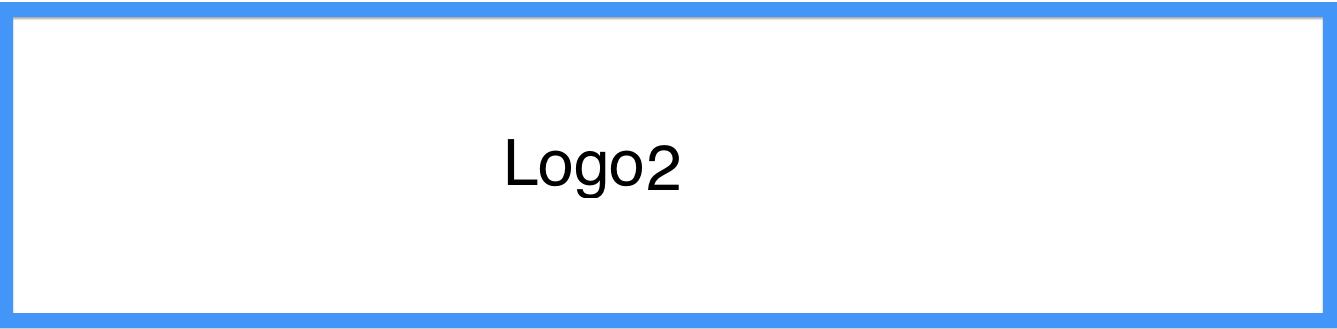
\includegraphics[width=0.3\textwidth]{abb/logo2}
\end{figure}
\vspace{-2cm}

\begin{verbatim}


\end{verbatim}

\begin{center}
\Large{Hochschule der Medien}\\
\Large{Fakultät für Druck und Medien}\\
\end{center}


\begin{center}
\Large{Medieninformatik}
\end{center}
\begin{verbatim}




\end{verbatim}
\begin{center}
\doublespacing
\textbf{\LARGE{\titleDocument}}\\
\singlespacing
\begin{verbatim}

\end{verbatim}
\textbf{{~\subjectDocument}}
\end{center}
%\begin{verbatim}\end{verbatim}
%\begin{center}\end{center}\begin{verbatim}\end{verbatim}
\begin{center}
\textbf{zur Erlangung des akademischen Grades \\ Bachelor of Science}
\end{center}
\begin{verbatim}






\end{verbatim}
\begin{flushleft}
\begin{tabular}{llll}
\textbf{Thema:} & & Deep Reinforcement Learning & \\
& &  \\
\textbf{Autor:} & & Nicolas Reinhart - nr034@hdm-stuttgart.de& \\
& & MatNr. 30038 & \\
& & \\
\textbf{Version vom:} & & \today &\\
& & \\
\textbf{1. Betreuer:} & & Prof. Dr.-Ing. Johannes Maucher &\\
\textbf{2. Betreuer:} & & M.Sc. Johannes Theodoridis &\\
\end{tabular}
\end{flushleft}


% römische Numerierung
\pagenumbering{arabic}

% 1.5 facher Zeilenabstand
\onehalfspacing

% Sperrvermerk
%\section*{Sperrvermerk}
\textcolor{red}{
Die vorliegende Arbeit beinhaltet interne und vertrauliche Informationen der Firma <Firmenname>.
Die Weitergabe des Inhalts der Arbeit im Gesamten oder in Teilen sowie das Anfertigen
von Kopien oder Abschriften - auch in digitaler Form - sind grundsätzlich untersagt.
Ausnahmen bedürfen der schriftlichen Genehmigung der Firma <Firmenname>.
}


%\newpage

% Einleitung / Abstract


%\section*{Zusammenfassung}
%&Hier steht der Text, welcher den Inhalte der Arbeit zusammenfasst...


\section*{Abstract}
\pagestyle{empty}
Heutzutage sind für viele Reinforcement Learning Benchmark-Umgebungen, wie Gym \cite{brockman2016openAI_gym} von openAI der Goldstandard. Das Team von Procgen, ebenfalls von openAI, ging noch einen Schritt weiter und implementiert für einige der Atari Spiele eine prozedurale Generierung der Level. Das allein führt bei einigen Algorithmen bereits zu besserer Sample Efficiency und einer besseren Generalisierung. 

In dieser Arbeit wird untersucht, wie sich eine visuelle Augmentation der Environments im Training oder während der Evaluation auf den allgemeinen Erfolg, den Reward und die Generalisierung auswirkt. Experimente mit maskierten Informationen oder invertierter Semantik untersuchen darüberhinaus die Relevanz bestimmter visueller Informationen und die Generalisierung von Konzepten.
Durchgeführt werden die Experimente im Chaser-Environment von Procgen. Dieses Spiel ist angelehnt an den Atari-Klassiker \dq Ms. Pac-Man\dq. Wie im Original ist es das Ziel, alle Orbs einzusammeln und auf dem Weg nicht von den Geistern gefressen zu werden.

Die Experimente der vorliegenden Arbeit zur farblichen Änderungen des Environments zeigen, dass bspw. die Existenz einer gewissen Farbe für die Erkennung eines Objekts große Relevanz besitzt, wenn das Objekt diese Farbe im Training hat. So nimmt die Performance eines Agenten rapide ab, wenn die Farbe der Orbs in der Evaluation eine andere ist, verglichen mit der zu Trainingsbedingungen. Des Weiteren zeigt sich über die Arbeit hinweg immer wieder, dass die Änderungen der Evaluationsumgebung und die daraus resultierenden Änderungen der Pixel-Verteilung, welche der Agent als Input bekommt, ebenfalls fatale Auswirkungen auf die Performance des Agenten haben. 

Experimente mit Änderung der Semantik von Objekten zwischen Training und Evaluation zeigen eindeutig, dass das der Architektur vorangestellte Convolutional Neural Network (CNN) stark auf die optische Erscheinung der Objekte fixiert ist. Das Vertauschen zweier Sprites stellt eine unüberwindbare Hürde für den Agenten dar. Die Feature Extraction des CNN scheint stark auf die Texturen und die Formen der jeweiligen Objekte angewiesen zu sein, um diese korrekt zu erkennen. So scheut sich der Agent, bei Experimenten mit invertierter Semantik der großen Orbs und der Geister, einen statischen Gegner einzusammeln - ein großen Orb, welcher ihn mit den Bewegungen eines Geistes verfolgt, wird hingegen gedankenlos eingesammelt. 


% einfacher Zeilenabstand
\singlespacing

% Inhaltsverzeichnis anzeigen
\newpage
\tableofcontents

% das Abbildungsverzeichnis
\newpage
% Abbildungsverzeichnis soll im Inhaltsverzeichnis auftauchen
\addcontentsline{toc}{section}{List of Figures}
% Verion 1: Abbildungsverzeichnis MIT führender Nummberierung endgueltig anzeigen
\listoffigures

% Verion 2: Abbildungsverzeichnis OHNE führende Nummberierung endgueltig anzeigen
%\begingroup
%\renewcommand\numberline[1]{}
%\listoffigures
%\endgroup


% das Tabellenverzeichnis
%\newpage
% Tabellenverzeichnis soll im Inhaltsverzeichnis auftauchen
\addcontentsline{toc}{section}{List of Tables}
% \fancyhead[L]{Abbildungsverzeichnis / Abkürzungsverzeichnis} %Kopfzeile links
% Tabellenverzeichnis endgültig anzeigen
\listoftables

%% WORKAROUND für Listings
%\makeatletter% --> De-TeX-FAQ
%\renewcommand*{\lstlistoflistings}{%
%  \begingroup
%    \if@twocolumn
%      \@restonecoltrue\onecolumn
%    \else
%      \@restonecolfalse
%    \fi
%    \lol@heading
%    \setlength{\parskip}{\z@}%
%    \setlength{\parindent}{\z@}%
%    \setlength{\parfillskip}{\z@ \@plus 1fil}%
%    \@starttoc{lol}%
%    \if@restonecol\twocolumn\fi
%  \endgroup
%}
%\makeatother% --> \makeatletter
% das Listingverzeichnis
%\newpage
% Listingverzeichnis soll im Inhaltsverzeichnis auftauchen
%\addcontentsline{toc}{section}{Listingverzeichnis}
%\fancyhead[L]{Abbildungs- / Tabellen- / Listingverzeichnis} %Kopfzeile links
%\renewcommand{\lstlistlistingname}{Listingverzeichnis}
%\lstlistoflistings
%%%%

% das Abkürzungsverzeichnis
% Abkürzungsverzeichnis soll im Inhaltsverzeichnis auftauchen
\addcontentsline{toc}{section}{List of Abbreviations}
% das Abkürzungsverzeichnis entgültige Ausgeben
\fancyhead[L]{List of Abbreviations} %Kopfzeile links
\nomenclature{GDA}{Generative Data Augmentation}
\nomenclature{SLP}{Single Layer Perceptron}
\nomenclature{MLP}{Multi Layer Perceptron}
\nomenclature{NN}{Neural Netzwerk}
\nomenclature{FFN}{Feed Forward Netzwerk}
\nomenclature{CNN}{Convolutional Neural Network}
\nomenclature{CNNs}{Convolutional Neural Networks}
\nomenclature{DNN}{Deep Neural Network}
\nomenclature{GAN}{Generative Adversarial Network}
\nomenclature{GANs}{Generative Adversarial Networks}
\nomenclature{MADGAN}{Multi-Agent Diverse Generative Adversarial Network}
\nomenclature{MADGANs}{Multi-Agent Diverse Generative Adversarial Networks}
\nomenclature{cGAN}{Conditional Generative Adversarial Network}
\nomenclature{cGANs}{Conditional Generative Adversarial Networks}
\nomenclature{DCGAN}{Deep Convolutional Generative Adversarial Network}
\nomenclature{DCGANs}{Deep Convolutional Generative Adversarial Networks}
\nomenclature{VAE}{Variational Auto Encoder}
\nomenclature{VAEs}{Variational Auto Encoders}
\nomenclature{FID}{Fréchet Inception Distance}
\nomenclature{IS}{Inception Score}
\nomenclature{batchnorm}{Batch Normalization}


%\nomenclature{}{}

\printnomenclature[3cm]


\newpage
\fancyhead[L]{\nouppercase{\leftmark}} %Kopfzeile links

% 1,5 facher Zeilenabstand
\onehalfspacing

% einzelne Abschnitte
\section{Introduction and Motivation}\label{introduction_and_motivation}
\pagestyle{fancy}
%\setcounter{page}{1}
\textit{Generative Adversarial Networks} (GANs) \cite{goodfellow2014generativeadversarialnetworks} and their variants revolutionized the field of computer vision in the year of 2014, enabling advacements in multiple areas of generating data. From \textit{Text to Image Synthesis} \cite{reed2016generativeadversarialtextimage}, \textit{Image Translation} \cite{isola2018imagetoimagetranslationconditionaladversarial}, \textit{Super Resolution} \cite{ledig2017photorealisticsingleimagesuperresolution}, \textit{Image Inpainting} \cite{pathak2016contextencodersfeaturelearning}, \textit{Style Transfer} \cite{wang2023multimodalityguidedimagestyletransfer} to \textit{Data Augmentation} \cite{shorten2019survey}, GANs have been used in a variety of applications.

% TODO: MORE REFERENCES HERE? - see mad gan main paper )(introduction) for more
The idea of using GANs for \textit{Generative Data Augmentation} (GDA) has already been applied successfully, e.g.: in computer vision \cite{Li2025comprehensivesurvedeepimages}, \cite{biswas2023generativeadversarialnetworksdata} or for creating music \cite{ji2020comprehensivesurveydeepmusic}. Especially the former survey \textit{A Comprehensive Survey of Image Generation Models Based on Deep Learning} has, along \textit{Variational Auto Encoders} (VAEs), a dedicated focus on GANs. Despite these achievements, in practice, GANs suffer from several challenges, complicating the training and inference process:

\begin{itemize}\label{problems_of_gans}
    \setlength{\itemsep}{-5pt}
    \item Mode Collapse
    \item Lack of inter-class Diversity
    \item Failure to Converge
    \item Vanishing Gradients \& Unstable Gradients
    \item Imbalance between Generator- and Discriminator Model
\end{itemize}

This thesis investigates the potential of using GANs - specifically \textit{Multi-Agent Diverse Generative Adversarial Networks} (MADGANs) \cite{ghosh2018madgan} - for Generative Data Augmentation. MADGANs aim to aid the first two of the afore mentioned in particular: Mode Collapse and Loss of inter-class Diversity. They, along other modifications, "\textit{propose to modify the objective function of the discriminator, in which, along with finding the real and the fake samples, the discriminator also has to correctly predict the generator that generated the given fake sample.}" \cite{ghosh2018madgan}. The goal of this adjustment of the discriminator is, that the discriminator has to push the generators towards distinct identifiable modes. While various strategies have been proposed to addrese mode collapse and inter-class diversity MADGANs explicitly enforce mode separation by introduction of multiple generators and the adjusted discriminator objective. This makes them particularly promising for GDA, as diverse samples and clear distinction of modes is crucial for training robust classifiers. In their paper, they experimentally show, that their architectural adjustment of GANs is generally capable of giving providing assistance for the first two of the mentioned problems.

The experiments in this work are structured into three major parts.

\paragraph{Set 1: Training and Analysis of GANs}  \label{thesis_goal_1}
The first set trains multiple variations of GANs, explicitly \textit{Deep Convolutional GANs} (DCGANs), \textit{Conditional GANs} (cGANs) and the afore introduced MADGANs, in addition to an adapted conditionalized version called \textit{Conditional Multi-Agent Diverse GANs} (cMADGANs) \ref{theoretical_cmadgan}. Here, the quality of the resulting images after training will be scored by the \textit{Fréchet Inception Distance} (FID) \cite{heusel2018ganstrainedtimescaleupdate} and the \textit{Inception Score} (IS) \cite{salimans2016improvedtechniquestraininggans}.

\paragraph{Set 2: Generating and Classifying Unlabeled Images}  \label{thesis_goal_2}
The second set uses the afore trained generative models to create images. Images without labels—images originating from MADGANs—will be classified using auxiliary classifiers trained with traditional data augmentation techniques.
The second instance the trained generative models are utilized to generate at least $6.000$ images per class. Since some architectures not non-conditional, pre-trained classifiers will be used to classify images. Specifically, data resulting from DCGANs and MADGANs have to be classified and given labels. 

\paragraph{Set 3: Training and Evaluating Classifiers}  \label{thesis_goal_3}
The third and most important set of experiments train classifiers using the generated and labeled samples. For this, stratified classifiers with different ratios of real to fake images are trained and evaluated on the respective validation set. These experiments are split into two scenarios: Replacement- and Expansion Scenarios. Their classification performance will be assessed using the \textit{F1 Score}.  \\

\noindent All of the above described is executed on the following datasets:
\begin{itemize}\label{used_datasets}
    \setlength{\itemsep}{-5pt}
    \item MNIST \cite{lecun2010mnist}
    \item Fashion MNIST \cite{xiao2017fashionmnist}
    %\item CIFAR10 \cite{Krizhevsky2009learning}
\end{itemize}


\paragraph{Aim of the Thesis}\label{aim_of_the_thesis}
This thesis evaluates the effectiveness of Multi-Agent Diverse GANs (MADGAN) for Generative Data Augmentation. First, the quality of generated samples is compared to those produced by a Deep Convolutional- and Conditional GAN. Further, a conditional adaptation of the MADGAN architecture is introduced and tested alongside already established methods. The quality of the resulting images is then evaluated utilizing the \textit{InceptionV3} model to calculate the Inception Score and FID of those images. Next, the sets of generated images are used to replace and alter training datasets for classifiers. The performances of the different classifiers are assessed by the F1 score. These sets of experiments are compared against traditional augmentations techniques, such as flipping, rotating and adding noise to the images, which serve as a minimum baseline. 

\noindent
With this experimental succession, this thesis studies the effect of the MADGAN-based data augmentation for subsequent classifiers, together with its conditionalized counterpart and comparing their performances against established traditional and generative augmentation techniques. 


\newpage


\section{Related Work}\label{related_work}

%AUGMENTATION

%##########################################
%##########################################



\newpage


\section{Theoretical Background}\label{body_theoretical_background}
This chapter serves as a reference for the theoretical background necessary to understand the insights gained in the following experimental chapters.
Section \ref{theoretical_classification} discusses classification models used to train on the extended dataset resulting from the generative augmentation process. In it, \textit{Neural Networks} (NNs) for image classification are introduced and the baselines for later comparisons are examined.
Sections \ref{theoretical_da} and \ref{theoretical_gda} establish the foundation for data augmentation and generative data augmentation.
Following sections \ref{theoretical_gan}, \ref{theoretical_dcgan}, \ref{theoretical_cgan}, and \ref{theoretical_madgan} provide theoretical knowledge necessary to understand the GAN architectures and their differences. The narrative follows their increasing complexity, starting from vanilla GANs, moving through deep convolutional GANs and conditional GANs, before diving into the background of multi-agent diverse GANs.
The final section (\ref{theoretical_image_scores}) explains the theory behind the Inception Score and Fréchet Inception Distance, concluding with an examination of the state-of-the-art \textit{InceptionV3} model used to compute them.
% ########################################################################################################
% # START: IMAGE CLASSIFICATION MODELS
% ########################################################################################################
\subsection{Image Classification Models}\label{theoretical_classification}
\subsubsection{Neural Networks for Classification}
Convolutional Neural Networks (CNNs) have become the dominant architecture for image classification tasks due to their inherent ability to automatically learn hierarchical features from raw pixel data. At their core, CNNs are build up by a sequence of convolutional-, pooling- and fully connected layers to extract hierarchical features, and funneling the information, typically into the \(N\) classes defined by the training data. That is, in case of classification tasks. 

Convolutional layers employ learnable filters to detect local patterns in the two-dimensional information. The two-dimensionality is inherent to image data. Pooling layers reduce the spatial dimensions, translating incoming data to a lower-dimensional space. Fully connected layers then map the extracted information into class probabilities, utilizing the \textit{Softmax} activation function. The afore mentioned layers are discussed in greater detail, in the following subsections.

\vspace{1em}

\textbf{Convolutional Layers}\label{theoretical_classification_conv_layers}
These layers compute the output from the local regions of the input. Let $(r \times c)$ be the two-dimensional input, e.g., a grayscale image, where $r$ represents the number of rows and $c$ the number of columns. Thus, $r \cdot c$ denotes the size of the image. Furthermore, let $(a \times b)$ be a filter with kernel size $a \cdot b$, where the filter is smaller than the input. This filter is moved from the top-left to the bottom-right over the input.

In each iteration, the dot product between the respective coefficients of the input region and the coefficients of the filter is computed. The product determines how much of the feature is present. The result of the dot product is then processed by the activation function $g$, which applies a non-linear transformation to it. If the activation function is ReLU, for example, only positive values are retained, meaning negative responses are set to zero. The result serve as an input to the subsequent layer.

The stride determines how far the filter moves after each operation. For a stride of $s = 1$, the filter can be placed in $(r - a + 1)$ positions along the height and $(c - b + 1)$ positions along the width, leading to an output size of $(r - a + 1) \times (c - b + 1)$. In general, the output size in the two-dimensional case is given by:
\[
\lfloor\left( \frac{r - a + s}{s} \right) \times \left( \frac{c - b + s}{s} \right)\rfloor
\]
where $\lfloor \cdot \rfloor$ denotes the floor function, which ensures that the output size is an integer.An image of this process can be found in Figure \ref{fig:maucher_convolutional_filtering}, in the Appendix. This image shows an input of size $[10 \times 10]$ and a filter of size $[3 \times 3]$. With a stride of $s = 1$, the resulting layer has a size of $[8 \times 8]$ (computed as $\left(10 - 3 + 1\right) \times \left(10 - 3 + 1\right)$). 

The stride of the filter can also be greater than $1$. Additionally, there is the option to apply padding to the image. There are different ways to implement padding. When padding of size $p$ is applied, the output size for a square input and filter is calculated as follows:
\[
\textbf{Output size} = \left\lfloor \frac{r - a + 2p}{s} \right\rfloor + 1
\]
A well known source for the context of convolutional arithmetic is the paper \textit{A guide to convolutional arithmetic for deep learning}, by Dumoulin et al. 2018 \cite{Dumoulin2016TransposedConv}. Convolutional layers are highly versatile due to their ability to process arbitrary numbers of input and output channels, enabling their widespread application across domains such as image processing, signal analysis, and natural language understanding.

\vspace{1em}

\textbf{Pooling Layers}\label{theoretical_classification_pooling_layers}
A pooling layer reduces the spatial dimensions (height and width) of feature maps, effectively compressing data while preserving the number of channels. Similar to convolutional layers, pooling layers apply a filter operations, that moves by a given stride. Instead of summing elements covered by the filter, typically, the filter applies one of the following operations: Max-, Average-, Global Max- or Global Average Pooling. \footnote{Other types of pooling involve e.g., L2-norm-, stochastic- or learnable pooling. However, these are less common than the afore mentioned types.}

To give an example, starting with an input of size $[32 \times 32 \times 10]$, applying a pooling operation with a $[2 \times 2]$ filter and a stride of 2 results in an output size of $[16 \times 16 \times 10]$. This operation reduces the spatial dimensions by half while keeping the depth unchanged.

\vspace{1em}

\textbf{Fully-Connected Layers}\label{theoretical_classification_fully_connected_layers}
Fully-Connected (FC), also called \textit{Dense} layer, typically computes the scores for the respective classes. In the case of ten classes, the result is a volume of size $[1 \times 1 \times 10]$\footnote{Typically, the output from the layer before the FC one is \textit{flattened} into a one-dimensional vector, preserving all information but removing spatial structure. For example, a $[2 \times 2]$ layer would result in a vector of size $[1 \times 4]$.}. By this stage, all spatial information has been transformed, leaving a quasi-one-dimensional vector. 

In a fully connected (FC) layer, each input is connected to each output, meaning every neuron in the previous layer is linked to every neuron in the FC layer. The output is computed as the weighted sum of all inputs, followed by an activation function, leading to the final classification scores that represent the likelihood of the input belonging to each class. It is not unusual to stack FC layers progressively to refine these scores. The spatial dimensions are collapsed into a single vector of class scores, which are then used for classification. The class probabilities are obtained by applying the Soft-Max Function \ref{theoretical_activations_softmax}.

\textbf{Batch Normalization Layers}\label{theoretical_classification_batchnorm_layers}
With their introduction in \textit{Batch Normalization: Accelerating Deep Network Training by Reducing Internal Covariate Shift} by Ioffe et al. \cite{ioffe2015batchnormalizationacceleratingdeep}, Batch Normalization (batchnorm) established as an integral part of convolutional networks and neural networks in general. This type of layer normalizes its inputs to subsequent layers and thereby stabilizing the distribution of activations throughout the training process. This reduces the internal covariate shift, allowing for higher learning rates and faster convergence. By normalizing activations, batchnorm helps prevent gradients from vanishing or exploding. However, it does not prevent it entirely. Additionally, it can provide regularization benefits and eliminate the need for Dropout, in some cases. With the afore mentioned benefits, batchnorm layers are particularly beneficial for deep learning networks with many layers.


\textbf{Typical Activation Functions in CNNs}

\begin{itemize}
    \item \textbf{ReLU (Rectified Linear Unit)}: \label{theoretical_activations_relu}
    \begin{equation}
    g(x) = \max(0, x)
    \end{equation}
    ReLU is the most widely used activation function in CNNs. It introduces non-linearity while maintaining efficiency by outputting zero for negative values and passing positive values unchanged.

    \item \textbf{Leaky ReLU}: \label{theoretical_activations_leakyrelu}
    \begin{equation}
        f(x) =
        \begin{cases}
        0 \quad \text{if } x < 0 \\
        x \quad \text{otherwise}
        \end{cases}
    \end{equation}
    A variant of ReLU, Leaky ReLU allows small negative values to flow through, addressing the \textit{dying ReLU} problem where neurons can become inactive \cite{Lu_Lu_2020}. 

    \item \textbf{Sigmoid (Logistic)}:  \label{theoretical_activations_sigmoid}
    \begin{equation}
        g(x) = \frac{1}{1 + e^{-x}}
    \end{equation}
    The sigmoid function squashes values between 0 and 1, commonly used for binary classification tasks. However, it can suffer from vanishing gradients for very large or small inputs.

    \item \textbf{Tanh (Hyperbolic Tangent)}:  \label{theoretical_activations_tanh}
    \begin{equation}
        g(x) = \frac{2}{1 + e^{-2x}} - 1
    \end{equation}
    Tanh outputs values between -1 and 1 and is similar to the sigmoid, but with a wider output range, making it more effective in many scenarios compared to sigmoid.

    \item \textbf{Softmax}: \label{theoretical_activations_softmax}
    \begin{equation}
        g(x_i) = \frac{e^{x_i}}{\sum_{j} e^{x_j}}
    \end{equation}
    Softmax is typically used in the output layer of CNNs for multi-class classification. It converts logits into probabilities, ensuring that the sum of the outputs is 1.

    \item \textbf{Cross-Entropy Loss:} \label{theoretical_loss_crossentropy}
    \begin{equation}
        g(y, \hat{y}) = -\sum_{i} y_i \log(\hat{y}_i)
    \end{equation}
    Cross-entropy is a common loss function for classification tasks. It measures the dissimilarity between the true label distribution \( y \) and the predicted probability distribution \( \hat{y} \). Lower values indicate a better alignment between the predicted and true classes. For consistency, the cross-entropy function is denoted with \( g \) here, although it is more commonly represented in the literature as \( H(y, \hat{y}) \) or \( H(p, q) \), where \( p \) refers to the true label distribution and \( q \) to the output of the discriminative model.


\end{itemize}

\subsubsection{Classification Models for augmented Training}
The classification models, on which the data augmentation is tested, are simple CNN classifiers consisting of the described layers. A dedicated classifier architecture is created for each dataset: MNIST and Fashion-MNIST (\ref{used_datasets}). The main differences between these architectures is the number of blocks, made of two-dimensional \hyperref[theoretical_classification_conv_layers]{convolutional}, \hyperref[theoretical_classification_batchnorm_layers]{batchnorm} and \hyperref[theoretical_classification_pooling_layers]{pooling} layers. All models use the \hyperref[theoretical_activations_relu]{ReLU} function for activation of the convolutional layers and the \hyperref[theoretical_activations_softmax]{Softmax} function for the activation at their last dense layer, resulting in probability distribution over the space of classes. More on the specific model architectures and used metrics for evaluation can be found in chapter \ref{body_prelim}.

\subsubsection{Classification Model Performance Metrics} \label{theory_classification_performanc_metrics}
For the assessment of classification performance, several standard metrics are commonly used. \textit{Accuracy} gives a measure for the overall proportion of correctly predicted instances, but can be misleading in imbalanced datasets. \textit{Precision} quantifies the proportion of correctly predicted positive instances among all predicted instances, whereas \textit{recall} \footnote{Recall is also known as sensitivity.} captures the proportion of correctly predicted positives out of all actual positive samples. 

The \textit{F1 score} is the harmonic mean of precision and recall and serves as a balanced metric when both false positives and false negative are of concern. This is especially useful for imbalanced datasets. Mathematically, the formulation of the F1 score is as follows: 

\begin{equation}
    \mathrm{Precision} = \frac{TP}{TP + FP}, \quad \mathrm{Recall} = \frac{TP}{TP + FN}
\end{equation}

\begin{equation}
    \mathrm{F1} = 2 \cdot \frac{\mathrm{Precision} \cdot \mathrm{Recall}}{\mathrm{Precision} + \mathrm{Recall}}
\end{equation}    

Even when working with stratified data, where class distributions are balanced, the F1 score remains valuable by providing a single, informative measure that accounts for the trade-off between precision and recall. Due to its sensitivity to both types of classification errors, the F1 score is used as the primary evaluation metric throughout this work, in the context of classifications.

% ########################################################################################################
% # END: IMAGE CLASSIFICATION MODELS
% ########################################################################################################

% ########################################################################################################
% # START: DATA AUGMENTATION
% ########################################################################################################

\subsection[Data Augmentation - DA]{Data Augmentation}\label{theoretical_da}
In this chapter, data augmentation (DA) techniques in the context of images are discussed in greater detail, starting with traditional augmentations (e.g., rotating or cropping an image) and ending with generative augmentations, in which generative models are used to expand the training data of subsequent classification models.

\subsubsection[Traditional Data Augmentation - TDA]{Traditional Data Augmentation}\label{theoretical_tda}
The need for data augmentation to make classification algorithms more resilient has existed for decades. Early papers mentioning the augmentation of data for classification tasks date back to the 1960s \cite{Nagy1966} (1966). For the context of deep learning, however, the augmentation of images was popularized by Krizhevsky et al. in 2012 \cite{Krizhevsky2012traditionaldataaugmentation}. This paper introduced the \textit{AlexNet}, a deep CNN used to classify images from the \textit{ImageNet} dataset \cite{ImageNetDataset5206848}, containing $1 000$ classes. 

%This paper also referenced the earlier work of Simard et al. from 2003 \cite{Simard2003bestpracticesforcnns}.

Generally, traditional data augmentation (TDA) techniques can be described as applying transformations to the initial training data. These transformations preserve the respective labels \(y\) and only act on the data \(X\). \footnote{It is to point out, that there are also transformations to be applied to the labels. This can include operations like random flipping of the labels. Such alterations also include techniques such as smoothing the labels, e.g., adjusting labels to not be strictly $0$ or $1$, but rather $0.1$ or $0.9$.} Applied transformations could either be used to enlarge the training data or to alter existing data i.e., altering the variability in it.\\

Augmentations are categorized based on the type of transformations applied:

\begin{itemize}
    \item \textit{Geometric Augmentation}: This category modifies the shape, position, and perspective: Rotation, Scaling, Flipping, Cropping, Shearing, Perspective Transform.
    \item \textit{Photometric Augmentation}: Alters pixel values while keeping the spatial structure: Brightness, Contrast, Hue Shift, Blurring
    \item \textit{Noise-Corruption Augmentation}: Imitates real-world degradations and distortions caused by cameras and sensors: Gaussian Noise, Speckle Noise, Salt-and-Pepper Noise.
\end{itemize}

\noindent
Mathematically, let \( X \) be an original data sample drawn from the dataset distribution \( P(X) \). Traditional data augmentation applies a transformation function \( f: X \mapsto \tilde{X} \), where \( f \) is a function sampled from a predefined set of augmentation operations \( \mathcal{F} \). The augmented data sample \( \tilde{X} \) is then given by:

\[
\tilde{X} = f(X), \quad f \sim \mathcal{F}.
\]

\noindent
Since TDA modifies already existing samples, the distribution of augmented samples \( P_{\tilde{X}} \) should ideally remain close to the original data distribution:

\[
P_{\tilde{X}}(X) \approx P(X).
\]

\noindent
In the context of data augmentation pipelines, this can be generalized as:

\[
\text{TDA}: (X, f) \mapsto \tilde{X}, \quad f \in \mathcal{F}.
\]

\begin{figure}[htbp]
    \centering
    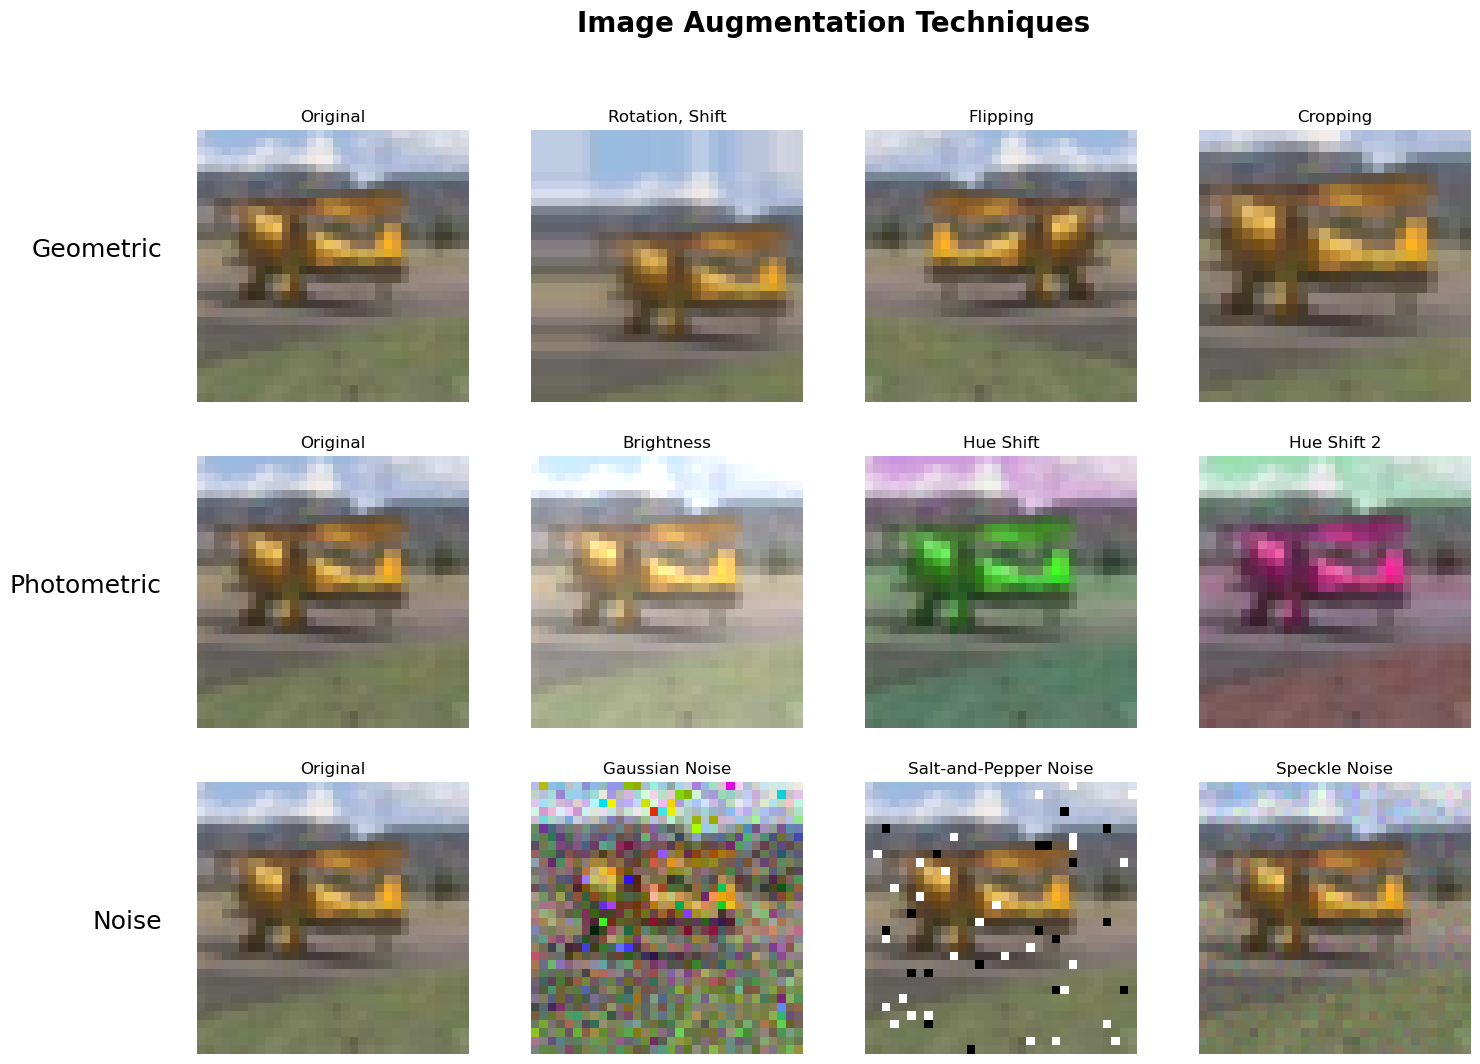
\includegraphics[width=.9\textwidth]{abb/traditional_image_augmentation_examples.png}
    \caption{Exemplary use of traditional augmentation techniques from the categories \textit{geometric} (first row), \textit{photometric} (second row), and \textit{noise-corruption} (third row). The image shown is an image from the \hyperref[used_datasets]{CIFAR10 dataset}, assigned to the class \textit{airplane}.}
    \label{fig:figure_tda_examples}
\end{figure}

\noindent
When applying the augmentations shown in Figure \ref{fig:figure_tda_examples}, it is mandatory to consider domain-specific knowledge and constraints. For example, flipping images from the MNIST dataset to train a generative model may result in an image where a horizontally flipped \textit{9} appears. This is in the domain of Arabic numerals semantically incorrect. Further, flipping a $9$ along horizontal and vertical axes would result in a $6$. Conversely, when classifying airplanes—which can vary in shape, color, three-dimensional orientation, and images may be taken through a dusty lens—applying most of the above augmentations could be beneficial, except for horizontal flipping, as mentioned above.


\subsubsection[Generative Data Augmentation - GDA]{Generative Data Augmentation}\label{theoretical_gda}
Differing from the previously mentioned TDA \ref{theoretical_tda}, generative data augmentation (GDA) techniques do not focus on altering existing data instances. Rather, it focuses on creating entirely new samples that match the underlying data distribution of the training data. These generated instances may or may not include labels.

The goal is to train a generative model \( G \) that produces instances \( X_1 \), for example, from a noise vector \( z \) \footnote{A noise vector may serve as input for a Generative Adversarial Network. See: \ref{theoretical_gan}}, such that the distribution of the generated data approximates the true distribution \( P(X) \) of the original dataset. In this context, \( G \) can be viewed as a function:

\[
G: z \mapsto X_1, \quad X_1 \sim P_G(X_{fake}) \approx P(X),
\]

\noindent
where \( P_G(X_{fake}) \) is the learned distribution of the generative model, aiming to approximate the real data distribution \( P(X) \).

In the case of \textit{conditional} generative data augmentation, additional information such as class labels \( y \) is incorporated into the generation process. This allows the model to generate samples corresponding to specific categories within the data. The conditional generative model \( G \) then follows:

\[
G: (z, y) \mapsto X_{fake}, \quad X_{fake} \sim P_G(X_{fake} \mid y) \approx P(X \mid y),
\]

\noindent
where \( P_G(X{fake} \mid y) \) represents the learned conditional distribution, aiming to approximate the real class-conditioned data distribution \( P(X \mid y) \). This can enable targeted data generation for specific categories, enhancing data diversity while maintaining class consistency.

% ########################################################################################################
% # END: DATA AUGMENTATION
% ########################################################################################################



% ########################################################################################################
% # START: Generative Aderserial Networks
% ########################################################################################################

\subsection[Generative Adversarial Network - GAN]{Generative Adversarial Network}\label{theoretical_gan}
Generative Adversarial Networks (GANs) have first been introduced by Goodfellow et al. in 2014 \cite{goodfellow2014generativeadversarialnetworks} GANs are a type of generative models designed to learn the underlying data distribution of their training data and generate new, realistic instances. The core idea of the framework is an adversarial training process between two neural networks (NNs): the \textit{Generator} \(G\) and \textit{Discriminator} \(D\), are competing against one another in a minimax game \cite{VonNeumann1928Minimax}. The following figure (\ref{fig:figure_gan_arch}) shows a visualization of the vanilla GAN architecture.

\begin{figure}[htbp]
    \centering
    \vspace{-4em}
    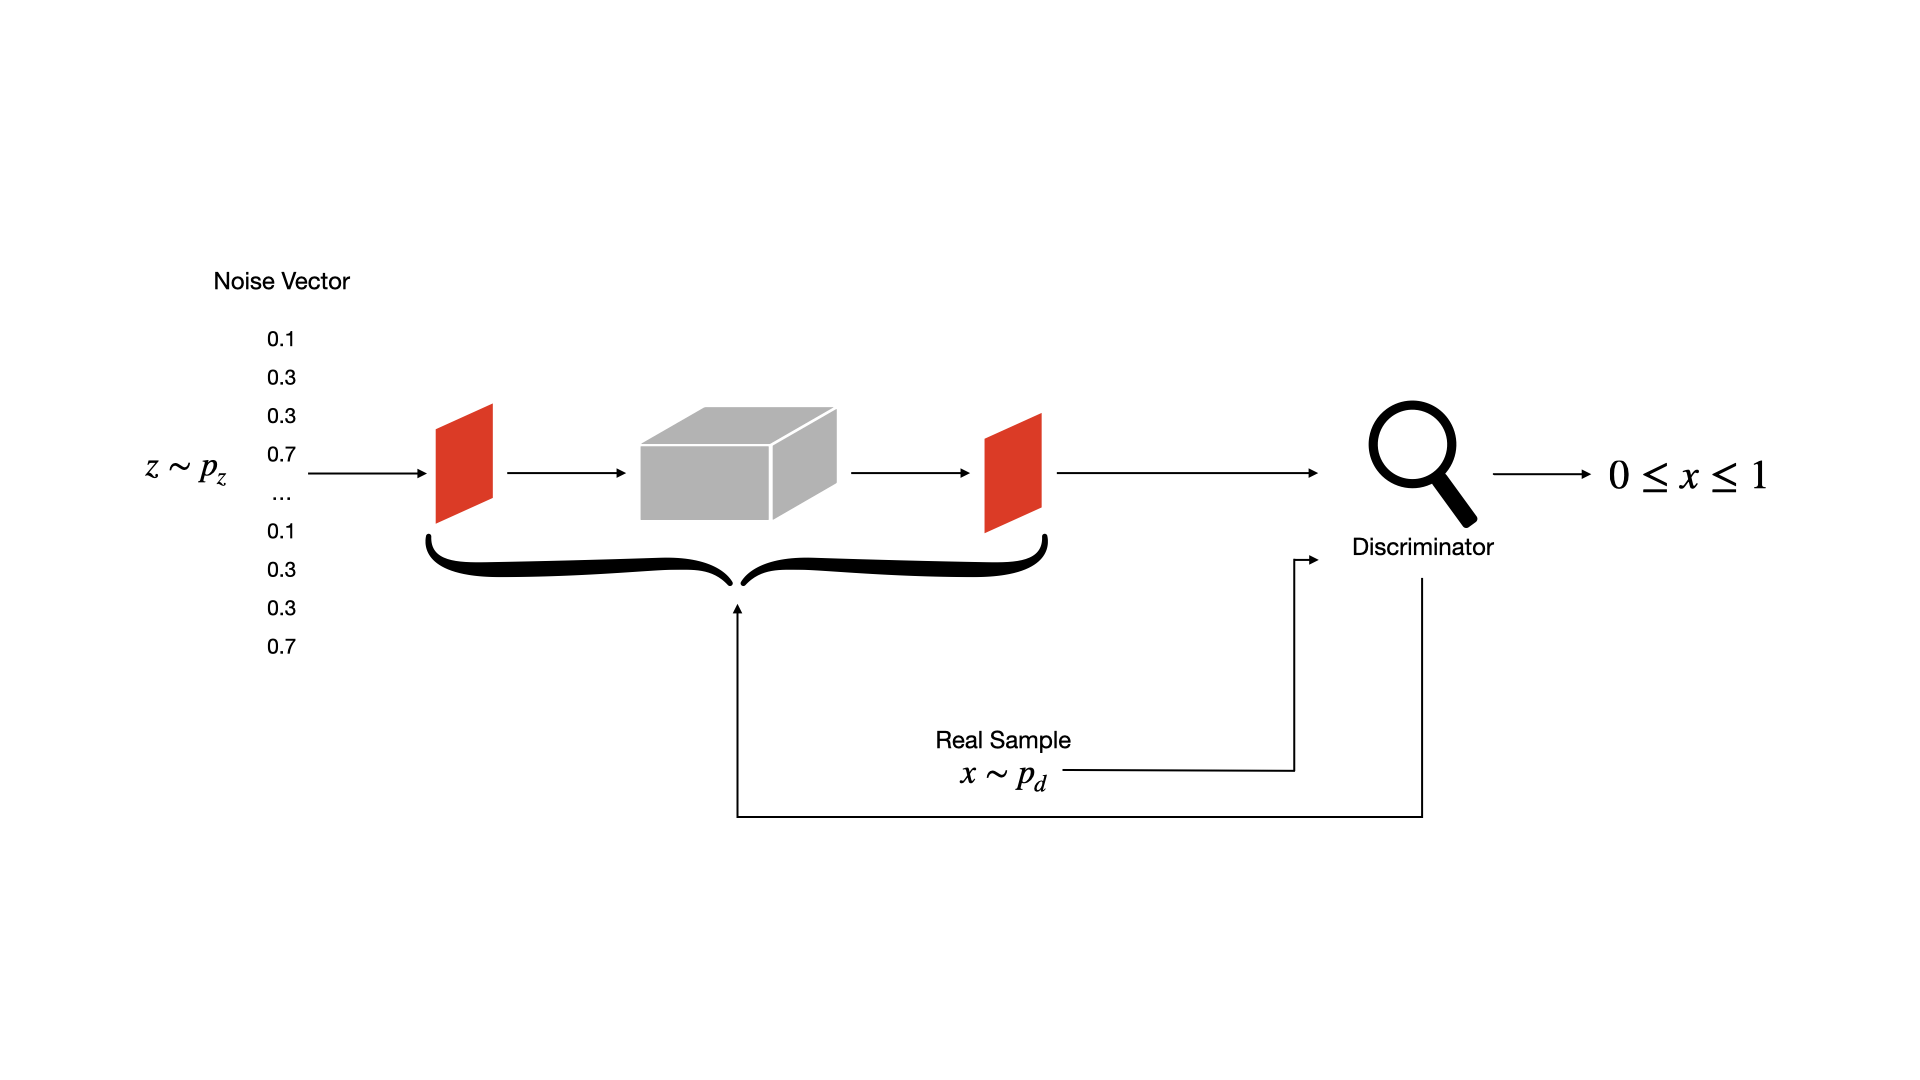
\includegraphics[width=.9\textwidth]{abb/arch_gan.png}
    \caption{Visualization of the vanilla GAN architecture. The figure shows the noise vector flowing into the generator. The generators output, as well as the real sample from \(P_{data}\), flow into the discriminator.}
    \label{fig:figure_gan_arch}
\end{figure}


\subsubsection{Mathematical Formulation}\label{theoretical_gan_math}
Let \(X \sim P_{data}\) be samples drawn from the real data distribution, and let \(z \sim P_z\) be random noise sampled from a known prior (e.g., a Gaussian or uniform distribution). The generator \(G\) is a function \(G(z): \mathbb{R}^{d_z} \to \mathbb{R}^{H \times W \times C}\), with \textit{H, W, C} as the height, width, and the number of channels, that maps a noise vector \(z\) to a synthetic data instance \(\tilde{X}\), attempting to approximate \(P_{data}\):\(\tilde{X} = G(z), \quad z \sim P_z.\)

The discriminator \(D\) is a function \(D: \mathbb{R}^{H \times W \times C} \to [0,1]\) that outputs the probability that a given sample is real or generated. It is trained to distinguish between real samples \(X \sim P_{data}\) and generated samples \(\tilde{X} \sim P_G\), where \(P_G\) is the implicit distribution induced by \(G\).

The training objective is formulated as the following minimax game:

    \begin{equation}\label{theory_gan_vanilla_formula}
        \mathcal{L}_{\text{adv}} = \min_G \max_D \mathbb{E}_{X \sim P_{data}} [\log D(X)] + \mathbb{E}_{z \sim P_z} [\log (1 - D(G(z)))].
    \end{equation}

Here, the discriminator \(D\) aims to maximize the probability of correctly identifying real samples \(D(X)\), with \(X \sim P_{data}\). The generator \(G\) aims to generate samples that fool \(D\), minimizing \(\log(1 - D(G(z)))\). In an ideal scenario, the game converges to a \textit{Nash equilibrium}, a concept from game theory. At this point, a stable state is reached where no player can benefit by unilaterally adjusting their strategy, assuming the other players keep their strategies unchanged. \(G\), in this case, produces samples indistinguishable from real data, i.e., \(P_G \approx P_{data}\). In this scenario, the discriminators output oscillates around $0.5$, continuously unable to differentiate real and fake samples.

\subsubsection{Training Process}\label{theoretical_gan_training}
GAN training follows an alternating optimization approach. Typically, alternating training the generator and the discriminator:
\begin{enumerate}
    \item Update \(D\): Given a batch of real samples from \(P_{data}\) and fake samples generated by \(G\), update \(D\) to maximize its ability to discriminate real from fake data.
    \item Update \(G\): Generate new fake samples and update \(G\) to minimize \\ \(\log(1 - D(G(z)))\), effectively pushing \(G\) to generate more realistic samples.
    \item Repeat the process iteratively, typically using stochastic gradient descent (SGD) or Adam optimization.
\end{enumerate}

\subsubsection{Challenges in GAN Training}\label{theory_gan_problems}
Next, challenges that can occur during the training of GANs are discussed. These have already been mentioned in the introductory section \ref{problems_of_gans}. Here, the afore mentioned challenges are described in detail.

\paragraph[Mode Collapse]{Mode Collapse}
Mode collapse occurs when the generator produces only a small subset of the data distribution, leading to a lack of diversity. Instead of generating varied diverse samples, it repeatedly produces similar ones that fool the discriminator. This happens when the generator finds an easy \textit{shortcut} rather than learning the full distribution over all classes. More formally, \(G\) collapses many values of \(z\) to the same value of \(x\) \cite{goodfellow2014generativeadversarialnetworks}. A common technique to mitigate this issue is minibatch discrimination \cite{salimans2016improvedtechniquestraininggans}. In several studies, experiments have been conducted to enhance diversity of GANs (\cite{Chang2024QDGenSampling}, \cite{Humayun2021MaGNET}, \cite{Humayun2022PolaritySampling}) % TODO: I tried minibatch discrimination for the cifar madgan, but did not work
\paragraph[Lack of Inter-Class Diversity]{Lack of Inter-Class Diversity}
Even if mode collapse is avoided, GANs may struggle to generate samples that represent all data classes equally. This is a common issue in class-conditional GANs, where samples across different classes may overlap or lack distinct features. Causes include imbalanced datasets, poor class conditioning, or weak discriminator feedback \cite{Odena201710.5555/3305890.3305954}.

\paragraph[Failure to Converge]{Failure to Converge}
Unlike traditional neural networks, GANs follow an adversarial training process, making optimization highly unstable. The loss functions of both the generator and discriminator change dynamically, often leading to non-convergent behavior. Methods like Wasserstein GANs (WGAN) \cite{arjovsky2017wassersteingan} and spectral normalization \cite{miyato2018spectralnormalizationgenerativeadversarial} improve stability and help achieve better convergence.

\paragraph[Vanishing & unstable Gradients]{Vanishing \& unstable Gradients}
When the discriminator becomes too strong, it perfectly distinguishes real from fake samples, leading to vanishing gradients for the generator. This prevents meaningful updates and stalling progress. On the other hand, unstable gradients cause erratic updates, preventing smooth learning. Alternative loss functions (e.g., LSGANs \cite{mao2017squaresgenerativeadversarialnetworks}) and spectral normalization can help stabilize the training.

\paragraph[Imbalance between Generator and Discriminator]{Imbalance between Generator and Discriminator}
A well-balanced GAN requires both models to improve at a similar pace. If the discriminator overpowers the generator, gradient updates to the generator can vanish. If it's too weak, the generator receives poor feedback and produces low-quality outputs \cite{goodfellow2014generativeadversarialnetworks}. Balancing techniques include adaptive learning rates, gradient penalties, and label smoothing \cite{Radford2015DCGAN}. Another interesting alternative, to tackle the problem of imbalance is introduced in the paper \textit{Progressive Growing of GANs for Improved Quality, Stability, and Variation} \cite{karras2018progressivegrowinggansimproved}.


\subsection[Deep Convolutional Generative Adversarial Network - DCGAN]{Deep Convolutional Generative Adversarial Network}\label{theoretical_dcgan}
Deep Convolutional Generative Adversarial Networks (DCGANs) were introduced by Radford et al. in 2015 \cite{Radford2015DCGAN} as an improvement over vanilla GANs. While the fundamental adversarial framework remains the same (see \hyperref[theoretical_gan_math]{3.3 Mathematical Formulation}, \hyperref[theoretical_gan_training]{3.3 Training Process}), DCGANs leverage deep convolutional neural networks to enhance stability and generate higher-quality images.

\subsubsection{Architectural Adjustments}\label{theorey_dcgan_architecture}
To improve training stability and image quality, DCGANs replace fully connected layers with convolutional layers, enabling enhanced spatial feature extraction. Following, the benefits of the layers for this context is briefly mentioned.

\begin{itemize}
    \item \textbf{Convolutional Architecture:} Fully connected layers in both \(G\) and \(D\) are replaced with deep convolutional layers, enabling better spatial feature extraction.
    \item \textbf{Strided Convolutions:} In the discriminator, pooling layers are removed in favor of strided convolutions, reducing the risk of information loss.
    \item \textbf{Transposed Convolutions:} The generator employs transposed convolutions (also known as fractionally-strided convolutions) instead of upsampling layers to improve the quality of generated images.
    \item \textbf{Batch Normalization:} Applied to both \(G\) and \(D\), batchnorm helps stabilize training by reducing internal covariate shift \ref{theoretical_classification_batchnorm_layers}. Batchnorm is omitted in the generators final layer to allow unrestricted output variability and in the discriminators input layer to preserve the original data distribution.
    \item \textbf{LeakyReLU Activation:} The discriminator uses LeakyReLU instead of standard ReLU to prevent dying neurons and allow gradients to flow through negative inputs \ref{theoretical_activations_leakyrelu}.
    \item \textbf{No Fully Connected Layers:} Fully connected layers are removed to maintain spatial coherence in generated images, as they discard spatial information by flattening feature maps. Instead, convolutional layers preserve local structures, enabling more realistic image synthesis \ref{theoretical_classification_fully_connected_layers}.
\end{itemize}


\subsection[Conditional Generative Adversarial Network - cGAN]{Conditional Generative Adversarial Network}\label{theoretical_cgan}

Conditional Generative Adversarial Networks (cGANs), introduced by Mirza and Osindero in 2014 \cite{mirza2014conditionalgenerativeadversarialnets}, extend the vanilla GAN framework by incorporating additional information \(y\), such as class labels, into both the generator and discriminator. This allows cGANs to generate samples conditioned on specific attributes, enabling controlled generation.

\subsubsection{Mathematical Formulation}
\label{theoretical_cgan_math}
The core idea of cGANs is to condition both the generator \(G\) and the discriminator \(D\) on auxiliary information \(y\). Instead of generating data solely from a noise vector \(z\), the generator now takes \(y\) as an additional input:

\begin{equation}
\tilde{X} = G(z, y)
\end{equation}

\noindent
Similarly, the discriminator receives both the real or generated sample and the corresponding condition:

\begin{equation}
D(X, y) \quad \text{and} \quad D(G(z, y), y)
\end{equation}

\noindent
The adversarial objective function for cGANs extends the standard GAN loss to incorporate this conditional dependency:

\begin{equation}\label{theory_gan_cond_formula}
\mathcal{L}_{\text{adv}} = \min_G \max_D \mathbb{E}_{X, y \sim P_{data}} [\log D(X, y)] + \mathbb{E}_{z \sim P_z, y \sim P_y} [\log (1 - D(G(z, y), y))]
\end{equation}

\noindent
This objective encourages the generator to produce samples that are not only realistic but also consistent with the provided condition, while the discriminator is trained to discern real from synthetic data based on their respective conditions.

\subsubsection{Architectural Adjustments}
\label{theory_cgan_architecture}
To implement cGANs, architectural adjustments are necessary compared to vanilla GANs:

\begin{itemize}
    \item \textbf{Input Conditioning:} Both the generator and discriminator must receive the conditional information \(y\) as input. This is typically achieved by concatenating the condition y with the noise vector z in the generator's input and with the input image \(X\) in the discriminators input.
    \item \textbf{Embedding Conditional Information:} For categorical conditions e.g., class labels, the condition \(y\) is often embedded into a lower-dimensional vector before concatenation. This embedding allows the network to learn meaningful representations of the conditions.
    \item \textbf{Concatenation, Addition, or Multiplication:} The conditional information can be incorporated through concatenation, addition, or element-wise multiplication at various layers within the generator and discriminator, depending on the specific application and architecture.
    \item \textbf{Preservation of Conditional Information:} Care must be taken, that the conditional information is preserved throughout the network. This means, that the information must traverse the network, all the way to the output layer.
\end{itemize}

\noindent
These architectural modifications ensure that the generator and discriminator can effectively utilize the conditional information to generate and discriminate samples based on the given conditions.

\subsection[Multi-Agent Diverse Generative Adversarial Network - MADGAN]{Multi-Agent Diverse Generative Adversarial Network}
\label{theoretical_madgan}
MADGAN is proposed as a generalized framework for the GAN architecture \cite{ghosh2018madgan}. The framework employs multiple generators, one discriminator and an adjusted objective for the discriminator. The adjusted objective aims to enforce the identifications of the generator creating given fake images \(G_{i} \hat{x}\). These changes specifically aim to ease the first two mentioned problems of GANs, namely \textit{Mode Collapse} and \textit{Lack of Inter-Class Diversity} \ref{theory_gan_problems}. This chapter delves into the specifics of this framework: integration of multi-agent systems with diversity-promoting techniques, within the GAN framework. The following subsections will detail the architecture, objective function, and training procedure of the MADGAN framework.

\begin{figure}[htbp]
    \centering
    \vspace{-4em}
    
\includegraphics[width=.9\textwidth]{abb/arch_madgan.png}
    \caption{Visualization of the MADGAN architecture. The figure shows the \(k+1\) outputs of the discriminator and the \(k\) generators, with tied weights in the middle of the network.}
    \label{fig:figure_madgan_arch}
\end{figure}


\subsubsection{Mathematical Formulation}
\label{theoretical_madgan_math}
As afore mentioned, the MADGAN architecture employs multiple generators and one discriminator. The goal for the \(K\) generators is to generate samples from different high probability regions of the data \(P_{data}\). In order to guide the generators into their respective direction, the objective of the discriminator has been modified. The objective no longer only has to differentiate between real and fake images, but also identify the generator that produced a given fake sample. Intuitively, the discriminator thereby forces the generators into mostly disjoint regions within the real data distribution. Inspired by the formulation for the discriminator in the paper \textit{Improved Techniques for Training GANs} \cite{salimans2016improvedtechniquestraininggans}, their discriminator model produces a \((k+1)\)-dimensional output vector using the \textit{Softmax} activation function (\ref{theoretical_activations_softmax}), where \(k\) is the number of generators. The output at index \(k+1\) represents the probability that the given sample belongs to the real data distribution \(P_{\text{data}}\), while the entries at indices \(j \in \{1, \ldots, k\}\) represent the probabilities that the sample originates from each of the \(k\) generators. The above Figure \ref{fig:figure_madgan_arch} shows a visualization of the architecture. Thus, when learning the discriminators parameters \(\theta_d\), the cross-entropy between the softmax outputs and the \textit{Dirac delta distribution} (Ddd) \(\delta \in \{0, 1\}^{k+1}\) is optimized. Here, \(\delta \in \{0,1\}^{k+1}\) is a one-hot vector defined as:

\[
\delta(i) = 
\begin{cases}
1, & \text{if the sample originates from the } i\text{-th generator, at positions:} \quad i \in \{1, \ldots, k\} \\
1, & \text{if the sample originates from } P_{\text{data}} \text{ at positions:} \quad i = k+1 \\
\end{cases}
\]
Since one of the above cases must be fulfilled, every other index in the resulting vector must be $0$. This means exactly one entry of \(\delta\) is 1, indicating the source of the sample.
Following this definition, the Ddd \(\delta\) can be understood as a one-hot encoding indicating whether a given sample is real of, and if not, from which generator it originates \footnote{It is important to point out, that the Dirac delta distribution is actually continuous. Their usage of the Ddd reminds of the Kronecker delta function, which \( \delta(i,j) = 1 \text{ for } i=j; 0 \text{ for } i \ne j \).}. The objective function for the optimization of \(\theta_d\), with \(\theta_g\) frozen is therefore:

\begin{equation}
    \max\limits_{\theta_d}\mathbb{E}_{x \sim p} H(\delta, D(x; \theta_d))
\end{equation}.

\noindent
\(H(...)\) here represents the negative cross-entropy function. Important to point out here is that, \textit{Intuitively, in order to correctly identify the generator that produced a given fake sample, the discriminator must learn to push different generators towards different identifiable modes.} \cite{ghosh2018madgan}, page 4. Figure \ref{fig:figure_madgan_diverse_mode_push} shows a visualization of the generators being pushed to different modes. This is explicitly encouraged in the discriminators objective function. The objective for the generators however, remains semantically the same as in the vanilla GAN \ref{theory_gan_vanilla_formula}. The difference here is that the objective function is generalized with an indexing \(i\) for the number of generators. That is, for the \(i\)-th generator, the objective function is to minimize:

\begin{equation}
    \mathcal{L}_{Gen_i} = \mathbf{E}_{x \sim P_{data}} [ \log D(X; \theta_d) ] + \mathbf{E}_{z \sim P_{z}} \log (1-D_{k+1}(G_i(z; \theta_{g}^{i}); \theta_x))
\end{equation}

\noindent\textbf{Enforcing Diverse Modes:}
The multi-agent framework by Ghosh et al. introduces a mechanism for promoting mode diversity through multiple generators. The core idea is formalized in \textbf{Theorem 1} \cite{ghosh2018madgan} (page 2), which demonstrates that, given an optimal discriminator, the \(k\) generators collectively form a mixture model.

The objective function for the set of generators, which they collectively minimize, is defined as:

\begin{equation}
\label{eq:madgan_gen_loss_original}
\mathcal{L}_{Gen_{[0...k]}} = \mathbf{E}_{x \sim P_{data}} [ \log D_{k+1}(X) ] + \sum_{i=1}^{k}\mathbf{E}_{x \sim p_{g_i}} [\log (1-D_{k+1}(x))]
\end{equation}

When the discriminator \(D_{k+1}\) reaches its optimal state for a given set of generator distributions, its output \(D^*_{k+1}(x)\) allows the generator's objective function to be re-expressed in terms of divergences between probability distributions. While the explicit algebraic steps are omitted for brevity in the paper \cite{ghosh2018madgan}, this transformation converts the cross-entropy terms in Equation \ref{eq:madgan_gen_loss_original} into a form involving Kullback-Leibler (KL) divergences. This is a standard technique in GAN proofs, where the problem of distinguishing \textit{real} from \textit{fake} becomes one of minimizing the \textit{distance} between distributions.

Specifically, at equilibrium, the generator objective boils down to minimizing:

\begin{equation}
\label{eq:madgan_theorem1_simplified}
\text{KL} \left( p_{data}(x) \| p_{avg}(x) \right) + k \cdot \text{KL} \left( \frac{1}{k}\sum_{i=1}^k p_{g_i}(x) \middle\| p_{avg}(x) \right) - (k+1)\log(k+1) + k\log k
\end{equation}
where \(k\) is the number of generators and \(p_{avg}(x) = \frac{p_{data}(x) + \sum_{i=1}^k p_{g_i}(x)}{k+1}\).

The key to understanding the constant term \( -(k+1)\log(k+1) + k\log k \) lies in how this transformed objective achieves its global minimum. This minimum value is reached precisely when the real data distribution \(p_{data}\) is perfectly matched by the average of the generator distributions, i.e., \(p_{data} = \frac{1}{k}\sum_{i=1}^{k} p_{g_i}\).

\noindent
Under this optimal condition (\(p_{data} = \frac{1}{k}\sum_{i=1}^{k} p_{g_i}\)):
\begin{enumerate}
    \item The average distribution \(p_{avg}(x)\) simplifies to \(p_{data}(x)\), as \\\(p_{avg}(x) = \frac{p_{data}(x) + k \cdot p_{data}(x)}{k+1} = \frac{(k+1)p_{data}(x)}{k+1} = p_{data}(x)\).
    \item Consequently, both KL-divergence terms in Equation \ref{eq:madgan_theorem1_simplified} become zero, as \(\text{KL}(P||Q) = 0\) if and only if \(P=Q\).
    \begin{itemize}
        \item \(\text{KL}(p_{data}(x) \| p_{avg}(x)) = \text{KL}(p_{data}(x)|\| p_{data}(x)) = 0\)
        \item \(k \cdot \text{KL}\left(\frac{1}{k}\sum_{i=1}^k p_{g_i}(x) \| p_{avg}(x)\right) = k \cdot \text{KL}(p_{data}(x) \| p_{data}(x)) = 0\)
    \end{itemize}
\end{enumerate}


Thus, at this global optimum, the generator's objective value is simply the constant term: \( -(k+1)\log(k+1) + k\log k \). This constant represents the baseline value of the divergence when the distributions are perfectly aligned, arising from the inherent mathematical structure of the objective function transformation.

It's significant to note that, for \(k=1\) (the case with a single generator), substituting \(k=1\) into this expression yields \( -(1+1)\log(1+1) + 1\log 1 = -2\log 2 + 0 = -\log 4 \). This value perfectly aligns with the known optimal value of the generator objective for the vanilla GAN, which is rooted in the Jensen-Shannon divergence as shown by Goodfellow et al. \cite{goodfellow2014generativeadversarialnetworks}. This consistency reinforces the correctness of Theorem 1.

The exact formulation of their theorem, proof, and propositions can be found in Ghosh et al. \cite{ghosh2018madgan}, following formulas (3) through (9).

\begin{figure}[htbp]
    \centering
    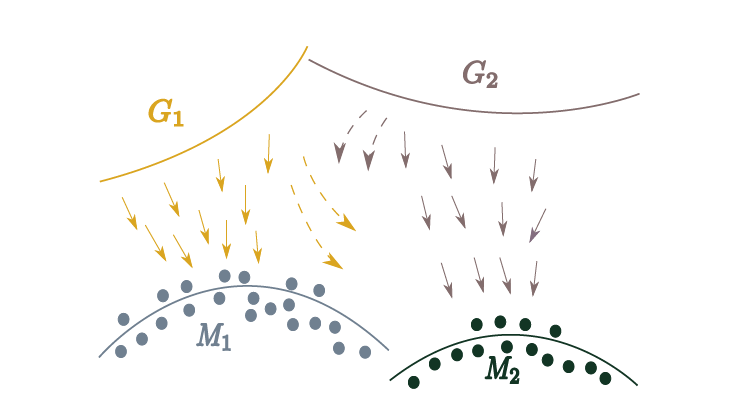
\includegraphics[width=.9\textwidth]{abb/madgan_diverse_mode_push.PNG}
    \caption{Figure taken from the original paper \cite{ghosh2018madgan}. The visualization shows how different generators \(G_ {1}\) and \(G_{2}\) are pushed to different modes \(M_{1}\) and \(M_{2}\), by the discriminator.}
    \label{fig:figure_madgan_diverse_mode_push}
\end{figure}

\subsubsection{Architectural Adjustments}
\label{theory_madgan_architecture}
The architectural changes can be summarized into three major changes applied to the vanilla GAN (\ref{theoretical_gan}) architecture:

\noindent\textbf{Multiple Generators:} The MADGAN architecture employs multiple generators instead of a single one. Following the intuition behind the adjusted discriminator objective, the outputs of the generators are distributed across different, mostly disjoint regions of the real data distribution.

\noindent\textbf{Modified Discriminator Objective:} The discriminator's last layer has an output of \(k + 1\), instead of \(1\)\footnote{Compared to the vanilla version of the architecture \ref{fig:figure_gan_arch}.} utilizing the softmax function \ref{theoretical_activations_softmax}. One output for every generator indicating whether an image originates from either one of the generator and one output implying if the discriminator came to the conclusion that the current image is fake or not. This encourages the discriminator to push the generators into identifiable distinct outputs (\ref{fig:figure_madgan_diverse_mode_push}).

\noindent\textbf{Parameter Sharing among Generators:} In the MADGAN architecture, the generators share all but the input and the final dense layer across the \(k\) generators. These shared layers function as a common feature extractor, reducing redundant computation in early feature extraction stages that capture high-frequency structures common to many datasets\footnote{For example, the first layers may detect horizontal and vertical edges, followed by corner detection, and so on.}. This setup is particularly recommended for single-view data, where the data distribution is more uniform. For multi-view data, however, parameter sharing is discouraged, as it may hinder each generator’s ability to learn mode-specific features.


% Define placeholder architectural functions
\newcommand{\definegenerator}{\texttt{define\_generator}}
\newcommand{\definediscriminator}{\texttt{define\_discriminator}}
% Define lambda symbol for diversity weight
\newcommand{\lambdadiv}{\lambda_{\text{div}}}
\subsection[Adapting MADGAN for Conditional Generation with Explicit Diversity - cMADGAN]{Adapting MADGAN for Conditional Generation with Explicit Diversity}
\label{theoretical_cmadgan}

The final goal of this research includes exploring methods for generating diverse samples in the mentioned datasets \ref{used_datasets} to be used for data augmentations. While the multi-agent framework by Ghosh et al. presents a potential approach, experiments revealed significant challenges in achieving stable training and satisfactory results in terms of image quality with the original method. Especially the CIFAR-10 dataset proved to be challenging, which is the only colored dataset used.

Consequently, an alternative framework, termed Conditional Multi-Agent Diverse GAN (cMADGAN), was conceptualized. The adjustment aims to retain the multi-generator diversity principle while simplifying the task of the discriminator. The discriminator model is rolled back to its original objective to differentiate between real and fake images. However, initial experiments indicated that this approach also faced convergence difficulties when applied to the original CIFAR-10 dataset. This specific is explained in more detail in the experiments section \ref{setup_cifar10_scope}.

The following sections detail the cMADGAN framework as implemented. This approach utilizes multiple generators ($G_1, \dots, G_K$), a single conditional discriminator ($D$) performing standard real/fake classification, and incorporates an explicit diversity loss between generator outputs alongside the adversarial objective.

\subsubsection{Mathematical Formulation}
\label{theoretical_cmadgan_math}

Let $z$ be a latent vector sampled from a prior distribution $p(z)$, typically a standard normal distribution. Let $c$ be the condition variable (e.g., class label) sampled from a distribution $p(c)$. The framework also employs $K$ generator networks $G_1, \dots, G_K$ and a single discriminator network $D$. Each generator $G_i$ maps an input pair $(z, c)$ to the data space, producing a fake sample $\hat{x}_i = G_i(z, c)$. The discriminator $D$ takes an input pair $(x, c)$ (where $x$ can be a real sample from the true data distribution $p_{\text{data}}(x|c)$ or a fake sample $\hat{x}_i$) and outputs a scalar probability estimating the likelihood that $x$ is real given the condition $c$.

The training involves optimizing two competing objectives, $\mathcal{L}_D$ for the discriminator and $\mathcal{L}_G$ for the generators:

\paragraph{Discriminator Loss:}
The discriminator is trained to distinguish real samples from fake samples generated by \textit{any} of the $K$ generators, given the condition $c$. Using the binary cross-entropy (BCE) loss, the objective is:
\begin{equation}
\label{eq:cmadgan_loss_d}
\begin{split}
\mathcal{L}_D = & - \mathbb{E}_{x \sim p_{\text{data}}(x|c), c \sim p(c)} [\log D(x, c)] \\
& - \frac{1}{K} \sum_{i=1}^{K} \mathbb{E}_{z \sim p(z), c \sim p(c)} [\log(1 - D(G_i(z, c), c))]
\end{split}
\end{equation}
This formulation averages the loss over the fake samples from all generators.

\paragraph{Generator Loss:}
The generators are trained collectively to fool the discriminator and simultaneously produce diverse outputs. The combined loss function for all generators includes an adversarial term and an explicit diversity term:
\begin{equation}
\label{eq:cmadgan_loss_g}
\mathcal{L}_G = \mathcal{L}_{\text{adv}} + \lambda_{div} \cdot \mathcal{L}_{\text{div}}
\end{equation}
where \(\lambda_{div}\) is a hyperparameter controlling the importance of the diversity component.

The components are defined as:
\begin{itemize}
    \item \textbf{Adversarial Loss ($\mathcal{L}_{\text{adv}}$):} Encourages generators to produce samples that the discriminator classifies as real. This is the sum of the non-saturating losses for each generator:
    \begin{equation}
    \label{eq:cmadgan_loss_g_adv}
    \mathcal{L}_{\text{adv}} = - \sum_{i=1}^{K} \mathbb{E}_{z \sim p(z), c \sim p(c)} [\log D(G_i(z, c), c)]
    \end{equation}

    \item \textbf{Diversity Loss ($\mathcal{L}_{\text{div}}$):} This term actively pushes the outputs of different generators apart. The goal during optimization ($\min \mathcal{L}_G$) is to maximize diversity. This is achieved by minimizing the negative cosine similarity. Cosine similarity is defined as:
    \begin{equation}
    \label{eq:cmadgan_cossim}
    \text{CosSim}(a, b) = \frac{\text{vec}(a) \cdot \text{vec}(b)}{\|\text{vec}(a)\|_2 \|\text{vec}(b)\|_2}
    \end{equation}
    where $\text{vec}(\cdot)$ denotes flattening the image tensor into a vector and $\|\cdot\|_2$ represents the \textit{L2 norm}, also known as the Euclidean norm of a vector. The diversity loss is the average pairwise negative cosine similarity, which the optimizer seeks to minimize:
    \begin{equation}
    \label{eq:cmadgan_loss_g_div}
    \mathcal{L}_{\text{div}} = -\frac{1}{N_p} \sum_{i=1}^{K} \sum_{j=i+1}^{K} \mathbb{E}_{z \sim p(z), c \sim p(c)} [\text{CosSim}(G_i(z, c), G_j(z, c))]
    \end{equation}
    where $N_p = K(K-1)/2$ is the number of unique generator pairs. Minimizing the combined $\mathcal{L}_G$ in Eq. \ref{eq:cmadgan_loss_g} thus encourages fooling the discriminator while explicitly promoting diversity between generator outputs.
\end{itemize}

\subsubsection{Architectural Adjustments}
\label{theory_cmadgan_architecture}

The cMADGAN architecture makes specific adjustments compared to both standard conditional GANs and the original MADGAN:

\begin{itemize}
    \item \textbf{Multiple Generators:}
    As the original MADGAN framework proposed, the cMADGAN employs $K$ distinct generator networks. As suggested in the original paper, the generators do not share their weights, due to the selection of datasets (cf. section 4.1 in \cite{ghosh2018madgan}). Each generator takes both the latent vector $z$ and the condition $c$ as input.
    \item \textbf{Conditional Discriminator:}
    Unlike the original MADGAN discriminator, the task of the cMADGAN discriminator performs the standard conditional GAN task \ref{theory_cgan_architecture}. $D$ receives an image $x$ (real or fake) and its corresponding condition $c$, and outputs a single probability indicating whether the image is real given the condition.
    \item \textbf{Conditioning Mechanism:} Class conditioning $c$ is integrated into both generator and discriminator networks.
        \begin{itemize}
            \item In the generators, an embedding of the condition $c$ is concatenated with the latent vector $z$ at the input layer before being processed by the main network layers (e.g., transposed convolutions).
            \item In the discriminator, the condition embedding is typically concatenated with intermediate feature maps before the final classification output, following common practices for conditional discriminators \cite{mirza2014conditionalgenerativeadversarialnets}.
        \end{itemize}
    \item \textbf{Explicit Diversity Enforcement:} Diversity is not solely an emergent property of competition but is explicitly encouraged via the $\mathcal{L}_{\text{div}}$ term in the generator objective (Eq. \ref{eq:cmadgan_loss_g}), directly penalizing high similarity between the outputs of different generators for the same input $(z, c)$.
\end{itemize}

The specific convolutional layers, normalization techniques, and activation functions within the generator and discriminator networks follow standard deep convolutional GAN (DCGAN) \cite{Radford2015DCGAN} principles and other relevant architectural patterns. This cMADGAN structure provides a framework for conditional generation that leverages multiple generators for diversity.


% ########################################################################################################
% # END: Generative Aderserial Networks
% ########################################################################################################


% ########################################################################################################
% # START: Image Scores
% ########################################################################################################

\subsection{Image Scores}\label{theoretical_image_scores}

To quantitatively evaluate the quality and diversity of images generated by generative models, several metrics have been proposed in the literature. These image scores aim to provide an objective measure to compare generative models independently of human evaluation. This section introduces widely-used metrics for evaluating generative models: \textit{Inception Score} (IS), \textit{Fréchet Inception Distance} (FID), and the underlying InceptionV3 model employed for these metrics.

\subsubsection[Inception Score - IS]{Inception Score}
The Inception Score (IS) \cite{salimans2016improvedtechniquestraininggans} is one of the earliest and most commonly used metrics for evaluating generative models, especially GANs. It leverages a pretrained InceptionV3 classifier to assess two main criteria of generated images:

\begin{itemize}
    \item \textbf{Image Quality (Clarity)}: Each generated image should be classified into a specific class with high confidence. This corresponds to a low-entropy conditional label distribution \( p(y|x) \).
    \item \textbf{Diversity}: Across the entire set of generated images, the distribution of predicted classes should be diverse and cover many labels. This corresponds to a high-entropy marginal label distribution \( p(y) \).
\end{itemize}

\noindent
Mathematically, the Inception Score is computed over a set of generated images \(x\) drawn from the generator's distribution \(p_g\):
\begin{equation}
IS = \exp \left( \mathbb{E}_{x \sim p_g} \left[ D_{\text{KL}}(p(y|x) \| p(y)) \right] \right)
\end{equation}
where \( D_{\text{KL}} \) denotes the Kullback-Leibler divergence between the conditional class distribution \(p(y|x)\) for a specific image \(x\) and the marginal class distribution \(p(y)\) estimated over all generated images. 

\noindent\textbf{Interpretation}:
A higher IS indicates that the model generates images that are confidently classified into diverse classes.

\noindent\textbf{Limitations of IS}:
\begin{itemize}
    \item Does not directly compare generated images with real images.
    \item Insensitive to intra-class diversity (e.g., generating only one type of dog within the dog class).
    \item Sensitive to the choice and specific training of the pretrained classifier.
\end{itemize}

\subsubsection[Fréchet Inception Distance - FID]{Fréchet Inception Distance}

The Fréchet Inception Distance (FID) \cite{heusel2018ganstrainedtimescaleupdate} improves upon IS by directly comparing the feature distributions of real and generated images. FID embeds both real (\(r\)) and generated (\(g\)) images into a lower-dimensional feature space using a pretrained \textit{InceptionV3} network (typically using the activations from the final average pooling layer, often referred to as 'pool3'). Each image is mapped to a fixed-length feature vector (embedding) consisting of all activation values from this layer. The embeddings across many images are then used to estimate two multivariate Gaussian distributions, one for real and one for generated data, by computing their empirical mean and covariance.


Let \( (\mu_r, \Sigma_r) \) and \( (\mu_g, \Sigma_g) \) denote the means and covariance matrices of the real and generated image Inception feature embeddings, respectively. The FID score is computed as the Fréchet distance (also known as Wasserstein-2 distance) between these two multivariate Gaussian distributions:
\begin{equation}
\text{FID} = \| \mu_r - \mu_g \|^2_2 + \text{Tr} \left( \Sigma_r + \Sigma_g - 2\left( \Sigma_r \Sigma_g \right)^{1/2} \right)
\end{equation}
where \( \|\cdot\|^2_2 \) is the squared \textit{L2 norm} (or Euclidean norm), \( \text{Tr}(\cdot) \) is the trace of a matrix, and \( \left( \Sigma_r \Sigma_g \right)^{1/2} \) denotes the **matrix square root of the matrix product** (i.e., standard matrix multiplication, not element-wise) between the two covariance matrices. The matrix square root \( A^{1/2} \) of a positive semi-definite matrix \( A \) is defined such that \( A^{1/2} A^{1/2} = A \).


\noindent\textbf{Interpretation}:
Lower FID indicates that the distribution of generated image features is more similar to the distribution of real image features, suggesting better quality and diversity. A score of 0 indicates identical distributions.

\noindent\textbf{Advantages over IS}:
\begin{itemize}
    \item Directly compares the generated image distribution to the real image distribution.
    \item More sensitive to intra-class mode collapse (lack of diversity within classes) as this affects \(\Sigma_g\).
    \item Generally found to correlate better with human judgment of image quality than IS.
\end{itemize}

\noindent\textbf{Limitations of FID}:
\begin{itemize}
    \item Assumes Gaussian distribution of features, which might be an approximation.
    \item Sensitive to the choice of feature extractor network and the specific layer used.
    \item Sensitive to both image quality (influencing feature representations) and diversity (influencing the mean and covariance of features).
    \item Requires a sufficiently large number of samples (both real and generated) for stable estimation of moments (\(\mu, \Sigma\)).
\end{itemize}

\subsubsection[InceptionV3 Model]{InceptionV3 for Image Evaluation}

Both IS and FID commonly rely on the InceptionV3 model~\cite{szegedy2016rethinking}, a deep convolutional neural network pretrained on the large-scale ImageNet dataset \cite{ImageNetDataset5206848}. The InceptionV3 network serves two primary roles in evaluating generative models:

\begin{enumerate}
    \item \textbf{Feature Extractor (for FID)}: Intermediate activations, typically from the final average pooling layer \textit{pool3}, are used as a semantic feature representation of the images. The statistics (mean and covariance) of these features are then compared between real and generated image sets.
    \item \textbf{Classifier (for IS)}: The output layer provides class probabilities for input images. These probabilities are used to calculate the entropy terms required for the Inception Score.
\end{enumerate}

\noindent\textbf{Properties of InceptionV3 relevant for image scoring}:
\begin{itemize}
    \item Trained on the diverse ImageNet dataset, providing a rich semantic feature space capable of capturing complex visual patterns.
    \item Uses fixed, non-trainable weights during evaluation, ensuring standardization and comparability of scores across different studies, provided the same implementation is used.
    \item The choice of layer for feature extraction (primarily for FID) impacts sensitivity; earlier layers capture lower-level features like texture, while later layers capture more abstract semantic information. The \textit{pool3} layer is commonly chosen as a balance.
\end{itemize}

\noindent\textbf{Limitations of using InceptionV3}:\label{theoretical_inception_model_limitaitions}
\begin{itemize}
    \item Domain Gap: The features learned on ImageNet (mostly natural images centered on objects) might not be optimally suited for evaluating images from significantly different domains, such as medical scans, satellite imagery, or abstract art.
    \item Sensitivity to ImageNet Classes: Performance, particularly for IS, can be less meaningful if the generated images depict objects or scenes vastly different from the $1 000$ ImageNet classes.
    \item Potential Bias: Potential biases present within the ImageNet dataset itself (e.g., representation bias) may be inherited by the features, potentially impacting evaluation fairness or relevance for specific target domains.
\end{itemize}


% ########################################################################################################
% # STOP: Image Scores
% ########################################################################################################

\newpage


\section{Preliminary Remarks}\label{body_prelim}

%##########################################
% How are the fid and is calculated? 
% Explain for all three datasets
%##########################################

%##########################################
% GAN TRAINING: whenever possible (excluding MNSIt), traditional data augmentation techniques: \ref{traditional_data_augmentation} have been applied to train the gans (all gans)
%##########################################




%# EXAMPLE OF FORMULA
%# \begin{quotation}
%# \centering
%#    \( A_t = \delta_t + (\gamma \lambda)\delta_{t+1} + ... + (\gamma \lambda)^{T-t+1} \delta_{T-1} \)
%# \end{quotation}












\newpage


\section{Experiments Setup}\label{body_experiments_setup}

\subsection{Preliminary Remarks}\label{body_prelim}
Before presenting the specific experiments and corresponding results in Chapter \ref{body_experiments_results}, this section outlines essential preliminary remarks. These remarks cover common configurations, definitions, and methodological aspects that apply across the subsequent experimental evaluations, providing necessary context and avoiding repetition later.

\subsubsection{Scope Limitation Regarding Standard CIFAR-10}
\label{setup_cifar10_scope}

The CIFAR-10 dataset, with its 32x32 pixel color images across 10 classes, represents a significant step up in complexity compared to MNIST or Fashion-MNIST and is a common benchmark in generative modeling. Consequently, initial plans involved evaluating the performance of multi-generator GAN approaches, including the original MAD-GAN \cite{ghosh2018madgan} and the adapted cMADGAN (Section \ref{theoretical_cmadgan}), on this standard dataset.

However, preliminary investigations encountered substantial difficulties in achieving stable training and generating samples of sufficient quality and diversity using these frameworks directly on standard CIFAR-10. Extensive efforts were undertaken to address these challenges, spanning a range of common techniques and modifications found in GAN literature. These included, but were not limited to:

\begin{itemize}
    \item Testing multiple generator and discriminator architectures with varying depths and capacities.
    \item Experimenting with different normalization layers (e.g., Batch Normalization, Spectral Normalization).
    \item Adjusting hyperparameters related to the Adam optimizer, particularly the learning rates for the generator(s) and discriminator, including various decay schedules and relative magnitudes.
    \item Implementing techniques designed to combat mode collapse and improve sample diversity, such as Mini-batch Discrimination.
    \item Tuning framework-specific hyperparameters like the latent dimension size and the diversity weight (\( \lambdadiv \)) for cMADGAN.
    \item Employing standard stabilization methods like label smoothing.
\end{itemize}

Despite these comprehensive attempts, persistent issues such as training instabilities (e.g., oscillating losses, vanishing or exploding gradients) or consistently poor quantitative results (e.g., low IS, high FID relative to benchmarks or simpler datasets) indicated that the models did not converge to a satisfactory performance level on the standard CIFAR-10 dataset within the practical constraints of this study.

Given that the primary focus of this thesis is to investigate the comparative effects of different GAN-based data augmentation strategies (including MADGAN and cMADGAN), a pragmatic decision was made to exclude the standard CIFAR-10 dataset from the main comparative experiments presented in the subsequent results chapters. This allows the analysis to focus on datasets (MNIST, Fashion-MNIST, and modified CIFAR-10) where the generative models achieved more stable and interpretable performance, enabling a clearer evaluation of the core research questions related to data augmentation effectiveness. The challenges encountered with standard CIFAR-10, while informative about the limitations of these specific multi-generator approaches on more complex data, are not subjected to further detailed analysis herein.

\subsubsection{Used Datasets}

\begin{table}[H]
    \centering
    \begin{tabular}{|c|c|c|p{7.5cm}|}
        \hline
        Dataset & N-Samples & Image Size & Description \\ \hline
        MNIST & 70,000  & $28 \times 28 \times 1$ & Grayscale images of handwritten digits (0–9). A classic benchmark for basic image classification tasks.\\ \hline
        Fashion-MNIST & 70,000  & $28 \times 28 \times 1$ & Grayscale images of clothing items. Provides more complexity and variability than MNIST, better reflecting real-world tasks.\\ \hline
    \end{tabular}
    \caption{Description of the used datasets for benchmarking.}
    \label{exp_setup_used_datasets}
\end{table}



\subsubsection{GAN: Architecture, Training and Data Augmentation}

\noindent\textbf{Architecture of the GANs}
In all experiments involving GAN models and their derivatives, the same network architecture has been employed for the \textit{MNIST} and \textit{Fashion MNIST} datasets. For initial experiments targeting the standard \textit{CIFAR-10} dataset (32, 32, 3), deeper architectures were utilized for both the generator and discriminator networks to account for the increased complexity of the data. However, for a specific set of experiments detailed in Section [todo: reference the correct section], where the CIFAR-10 dataset was modified (28, 28, 1) to facilitate analysis, architectures comparable to those used for MNIST/Fashion MNIST were employed. These proofed to result in mostly stable training. The specific architecture relevant to each experiment will be reiterated in its respective section.\\

\noindent\textbf{Training}
For training all GAN-based models, including DCGAN, cGAN, MADGAN and cMADGAN, the \textit{Adam} optimizer has been utilized. The learning rate follows an exponentially decaying schedule throughout the training process.\\

\noindent\textbf{Data Augmentation}\label{body_experiment_dataaugmentation}
To increase the diversity of the training data for both generator and discriminator models, several traditional augmentation techniques have been applied. These include horizontal flips, brightness and contrast adjustments, and the addition of Gaussian noise.
Horizontal flips are applied with a probability of \(50\%\), except for the \textit{MNIST} dataset, where flips are omitted due to the semantic relevance of digit orientation. Brightness and contrast adjustments are always applied within a uniform range of \([-0.1, 0.1]\). Gaussian noise is added by sampling from a normal distribution with mean \(0\) and standard deviation \(0.05\). Finally, the augmented images are clipped to the valid value range of \([-1, 1]\).

\subsubsection{Stratified Classifiers as measure for augmentation Quality}
To definitively evaluate the quality of the GDA, the fake images are used to replace and exapnd the underlying original datasets and train classification models on them. For this, the training datasets are specifically creafted to contain different ratios of real to fake images. To avoid biasing one class in the datasets over another, the datasets are stratified with respect to the number of samples per class. \footnote{Out of the used datasets, only the MNIST dataset is not originally stratified.}

\subsubsection{Labeling unconditioned data}\label{body_experiment_labeling_data}
Due to the fact, that multiple experiment using unconditioned GANs were executed (\ref{exp_results_research_questions}), many images have been created with no corresponding label to them. To classify the unlabeled data, simple CNN classifiers, with adequate TDA, were utilized. The applied augemntations techniques are the as follows: horizontal- and vertical shift by 0.1 relativ to the absolute size of the image, rotation of up to 15 degree and vertical flipping. As afore mentioned, flipping images along the vertical axes is omitted for the MNIST dataset, due to semantical invalidity. Graphical depictions of the classiers used can be found in the appendix (\ref{appendix_classifiers}). The auxiliary classifiers were optimized for their Accuracy on the held-out test set of the respective dataset.\\


\subsubsection{Utilization of InceptionV3 for FID and IS}\label{body_experiment_inception_model}
It is crucial to note that the significant differences between the ImageNet domain (high-resolution, color, 1000 object classes) and datasets commonly used in GAN research like MNIST, Fashion-MNIST (low-resolution, grayscale), or CIFAR-10 (low-resolution, color, 10 simpler classes) represent a substantial domain gap \ref{theoretical_inception_model_limitaitions}. This gap may limit the effectiveness or absolute interpretability of InceptionV3-based scores for these specific datasets. Furthermore, due to the sensitivity of these scores to implementation details (e.g., image resizing methods, specific InceptionV3 weight versions), a direct comparison of scores calculated here to those from external literature is generally unreliable unless the evaluation methodology is verified to be identical. Therefore, within this thesis, IS and FID scores are primarily utilized for relative comparisons between the different models and experiments conducted herein, rather than for absolute benchmarking against potentially disparate external results. This context warrants careful consideration when analyzing the experimental outcomes presented later.


\subsection{Experimental Workflow}\label{body_experiment_succession}

The evaluation of each generative model adhered to a consistent experimental workflow, outlined below:

\begin{enumerate}
    \item \textbf{GAN Training:} The specific generative model (e.g., DCGAN, cGAN, MADGAN, cMADGAN) was trained on the target dataset. Model performance during training was monitored using predefined metrics such as FID and IS.

    \item \textbf{Synthetic Sample Generation (Per Generator):} After training, the individual generators \(G_i\) / \(G_{i, j}\) within the trained model (where \(i=1\) for single-generator models like DCGAN/cGAN, and \(i=1...K, j=0...(K-1)\) for multi-generator models MADGAN/cMADGAN with \(K \in \{3, 5, 7, 10\}\)) are used to create a distinct set of synthetic images, denoted as \(S_{\text{fake}, i}\). For each class in the original dataset, at least $6.000$ images are generated by each generator \(G_i\), resulting in \(K\) separate datasets of synthetic samples for each trained multi-generator model.
        \begin{itemize}
            \item \textit{Labeling Unconditional Samples:} For samples generated by unconditional models or generators (DCGAN, MADGAN generators), class labels are assigned to the images within each respective set \(S_{\text{fake}, i}\) using the pre-trained classifiers detailed in Section \ref{body_experiment_labeling_data}.
        \end{itemize}

    \item \textbf{Downstream Classifier Training (GDA Evaluation - Per Generator):} The effectiveness of Generative Data Augmentation (GDA) was evaluated separately for each generator \(G_i\) / \(G_{i, j}\) of a trained GAN-based model, using its corresponding synthetic sample set \(S_{\text{fake}, i}\) / \(S_{\text{fake}, i, j}\). For single-generator models, this step was performed once using \(S_{\text{fake}, 1}\). Using a fixed classifier architecture specific to each dataset trained for $50$ epochs, classifiers are trained under two distinct augmentation scenarios for each sample set \(S_{\text{fake}, i}\):
        \begin{itemize} \label{exp_setup_difference_replace_expand}
            \item \textit{Replacement Scenario:} This assessed the utility of synthetic data from generator \(G_i\) as a substitute for real data. Training commenced with a baseline classifier using $5.000$ real images per class. In subsequent steps, the number of real images per class was decreased by $1.000$ while the number of synthetic images per class (drawn from \(S_{\text{fake}, i}\)) was increased by $1.000$, maintaining a constant dataset size of $5.000$ images per class. This process continued until the final classifier was trained solely on $5.000$ synthetic images per class from \(S_{\text{fake}, i}\).
            \item \textit{Expansion Scenario:} This evaluated synthetic data from generator \(G_i\) as a supplement to real data. Training started with the same baseline ($5.000$ real images per class). The real dataset was then augmented by adding synthetic images from \(S_{\text{fake}, i}\) in increments of $1.000$ per class per step, reaching a maximum of $5.000$ synthetic images per class. The final classifier in this scenario was trained on a combined dataset of $5.000$ real and $5.000$ synthetic images per class from \(S_{\text{fake}, i}\).
        \end{itemize}
      Note that for each trained MADGAN or cMADGAN model with K generators, the full set of Replacement and Expansion classifier training experiments was performed K times, once for each generator's synthetic dataset.

    \item \textbf{Downstream Classifier Evaluation:} The performance of all trained classifiers (baseline and those from the replacement and expansion scenarios for each generator set \(S_{\text{fake}, i}\)) was evaluated using predefined classification metrics [TODO: Add reference to metrics definition, e.g., Section X.Y on Evaluation Metrics]. Results for multi-generator models may be presented as averages across the K generators or by selecting representative examples of specific generators with specified ratios between real and fake images.
\end{enumerate}

\noindent In total, this setup results in $44$ (datasets (2) * augmentation types (4) * experiment setup (2) * n-generators trained ([3, 5, 7, 10])) experiment sets. Taking the different ratios of real to fake images in the expansion / replacement scenarios into account, a total of $1.166$ separate classifiers were trained to evaluate the potential of multi-agent architecture for GDA.

\subsection{Comparison of Classifier Performance}
Due to the fact that the MADGAN and cMADGAN architectures apply a multi-agent strategy i.e., training multiple generators for one model, only the best run is selected for direct comparison to others. For example, when comparing MADGAN to cMADGAN in \ref{exp_results_ans_q4}, the best performing subset of the respective GAN architecture is used for comparison. The rest of the experiments not discussed explicitly or only mentioned can be seen in the appendix \ref{app_strat_class_performance}.

\subsection{Hardware and Software Environment}

\subsubsection{Hardware}
All models trained in the context of this thesis were trained utilizing the \textit{Deeplearning Cluster} provided by the \textit{Hochschule der Medien - Stuttgart}. The cluster provides 8 nodes that with dedicated graphics cards supporting the \textit{CUDA} framework. The specific machines deployed in the cluster can be seen here \href{https://deeplearn.pages.mi.hdm-stuttgart.de/docs/}{Deeplearn cluster Documentation}\footnote{Link to the documentation for print versions: \url{https://deeplearn.pages.mi.hdm-stuttgart.de/docs/}.}.

\subsubsection{Software}
The code for the experiments was developed with the programming language python, using version \(3.9\). Models are based on the tensorflow ecosystem. The exact packages and their respective version can be found here \href{https://github.com/N10100010/mad_gan_thesis/blob/main/code/server_env.yml}{Aanconda environment}\footnote{Link to the environment file for print versions: \url{https://github.com/N10100010/mad_gan_thesis/blob/main/code/server_env.yml}.}.



\newpage


\section{Experiments Results}\label{body_experiments_results}
\paragraph{Motivation}\label{exp_results_motivation}
The primary motivation for investigating multi-generator GAN architectures for Generative Data Augmentation (GDA) stems from a suggestion by Ian Goodfellow on the Lex Fridman Podcast \cite{fridman2019Goodfellow}. He proposed leveraging the diversity inherent in multiple generative models trained on the same data to potentially improve downstream classifiers:

\begin{quotation}
    \noindent So one thing I think is worth trying [\dots] is, what if you trained a whole lot of different generative models on the same training set, create samples from all of them and then train a classifier on that. Because each of the generative models might generalize in a slightly different way, they might capture different axes of variation, that one individual model wouldn't and then the classifier can capture all of those ideas, by training on all of their data.
\end{quotation}\citep[50:37]{fridman2019Goodfellow}

\noindent Goodfellow's concept resonates strongly with the principles of Multi-Agent Diverse GANs (MADGANs) \cite{ghosh2018madgan}. The MADGAN architecture, with its explicit diversity-promoting objective and use of multiple generators, provides a suitable framework for realizing this augmentation strategy. Therefore, the work by Ghosh et al. laid the conceptual groundwork for this thesis.

\subsection{Key Research Questions} \label{exp_results_research_questions}
This chapter investigates the following questions regarding MADGANs for data augmentation:
\begin{itemize}
    \item \textbf{Question 1}: How do the FID- and Inception Score compare between the generative methods?
    \item \textbf{Question 2}: Does Generative Data Augmentation (GDA) with MADGANs enhance downstream classifier performance more effectively than Traditional Data Augmentation (TDA)?
    \item \textbf{Question 3}: How does the performance enhancement achieved with MADGAN-based GDA compare to that of GDA using standard GANs or conditional GANs?
    \item \textbf{Question 4}: How does the performance enhancement achieved with MADGAN-based GDA compare to that of cMADGAN-GDA?
    \item \textbf{Question 5}: What is the impact of varying the number of MADGAN generators on downstream classifier performance?
\end{itemize}

\subsection{Key Research Question Answers}
As mentioned in the subchapter about the experimental workflow, four sets of multi-agent generators models were trained  for the MADGAN and cMADGAN architectures (\ref{body_experiment_succession}). The four sets differ by \(K\), the number of generators trained, with \(K \in [3, 5, 7, 10]\). Onward, the generator of a discussion is identified explicitly by a suffix referencing the generator of a trained set \(G_{i, j}\) with \(i=K, j=0...(K-1)\) (e.g., \(\text{MADGAN}_{5, 0}\) for the first generator in the architecture trained with five generators). The set of generators however, is referenced via the notation: MADGAN \(K=5\) (e.g., if a discussion talks about the average performance of the generators \(0...4\)). Throughout this chapter, the experiment will be viewed with respect to afore mentioned differentiation between expansion and replacement scenarios \ref{exp_setup_difference_replace_expand}. The comparisons of FID- and Inception Score are excluded from this differentiation. Experiment not directly discussed in greater detail can be seen in the appendix \ref{app_strat_class_performance}.
The generated graphs contain all respective runs of a given experimental setup for which, best, worst, average, median, and baseline are explicitly highlighted. Each gray line in a graph, that is not highlighted represents every other combination of the setup. Especially for the multi-agent generator setups, this results in many graphs, up to $60$ per figure. Therefore, a colorful highlighting of specific graphs is omitted as this would not benefit the overall readability of the respective graphs. This however removes the potential for interesting insights. TODO: maaah, important sentence... Could be phrased better


\subsubsection[Question 1]{Comparison of FID- and Inception Scores}     \label{exp_results_ans_q1}
In order to compare the FID-Score and the means and standard deviations of the IS, $10.000$ generated samples are chosen by random selection. These fake images are drawn from the entirety of the generated data for a given generator, regardless of their assigned class.
The comparison is being based on the respective datasets used (MNIST, Fashion-MNIST) for data generation.\\
\\
\noindent\textbf{MNIST Dataset}
\begin{table}[H]
    \centering
    \begin{tabular}{|c|c|c|c|c|c|}
        \hline
        Generator Type & Generators trained & FID & IS & IS-std \\
        \hline
        DCGAN & 1 & $122.097$ & $\mathbf{2.611}$ & $0.056$ \\
        \hline
        cGAN & 1 & $28.721$ & $2.553$ & $0.022$ \\
        \hline
        MADGAN & K=3 (avg) & $23.177$ & $2.511$ & $0.04$ \\
        \hline
        MADGAN & K=5 (avg) & $22.656$ & $2.471$ & $0.044$ \\
        \hline
        MADGAN & K=7 (avg) & $21.599$ & $2.533$ & $0.051$ \\
        \hline
        MADGAN & K=10 (avg) & $\mathbf{20.973}$ & $2.474$ & $0.037$ \\
        \hline
        cMADGAN & K=3 (avg) & $25.578$ & $2.398$ & $0.036$ \\
        \hline
        cMADGAN & K=5 (avg) & $29.071$ & $2.35$ & $0.039$ \\
        \hline
        cMADGAN & K=7 (avg) & $30.645$ & $2.354$ & $0.039$ \\
        \hline
        cMADGAN & K=10 (avg) & $110.553$ & $2.062$ & $0.018$ \\
        \hline
    \end{tabular}
    \caption{FID and IS results for GAN models on MNIST, comparing single-generator (DCGAN, cGAN) and multi-generator (MADGAN, cMADGAN; K=3-10) approaches.}
    \label{tab:exp_mnist_fid_is}
\end{table}
\textbf{Interpretation:} Table \ref{tab:exp_mnist_fid_is} presents the Fréchet Inception Distance (FID, lower is better) and Inception Score (IS, higher is better) for various GAN models evaluated on the MNIST dataset. The results reveal a trade-off between the two metrics across different architectures.

The baseline DCGAN achieved the highest IS ($2.611$) but performed poorly in terms of FID ($122.097$). Introducing conditioning via cGAN significantly improved the FID to $28.721$ while maintaining a high IS ($2.553$). The results for the DCGAN point to an eventual mode collapse. A histogram of the resulting labels from this data generation can confirm the mode collapse\footnote{A histogram of the resulting labels originating from the generation process of the DCGAN on MNIST can be found here \ref{fig:figure_dcgan_datacreation_histogram}.}.

For unconditional models, the multi-generator MADGAN framework consistently yielded better FID scores than the baselines. Furthermore, MADGAN's FID improved monotonically as the number of generators increased, achieving the best overall FID of $20.973$ with 10 generators. However, its IS scores ($~2.5$) were slightly lower than the single-generator baselines.

The conditional multi-generator adaptation, cMADGAN, showed a more complex relationship with the number of generators (K). It performed very poorly for K=3 (FID $110.553$) but improved substantially at K=5, achieving a competitive FID ($25.578$) - better than cGAN - albeit with a lower IS ($2.398$). Contrary to MADGAN, increasing generators beyond K=5 resulted in worse FID scores for cMADGAN ($29.071$ for K=7, $30.645$ for K=10). Consequently, for K>=5, the unconditional MADGAN consistently outperformed cMADGAN in FID within these experiments.

In summary, on MNIST, standard conditioning (cGAN) greatly enhances baseline FID. The unconditional MADGAN framework effectively improves FID further, benefiting from more generators. The conditional cMADGAN variant demonstrates potential (peaking at K=5) but exhibits non-monotonic FID performance with increasing generator count in this setup, suggesting a more complex optimization landscape compared to its unconditional counterpart. \\

\noindent\textbf{Fashion-MNIST Dataset}
\begin{table}[H]
    \centering
    \begin{tabular}{|c|c|c|c|c|c|}
        \hline
        Generator Type & Generators trained & FID & IS & IS-std \\
        \hline
        DCGAN & 1 & $25.56$ & $4.21$ & $0.099$ \\
        \hline
        cGAN & 1 & $123.349$ & $3.573$ & $0.117$ \\
        \hline
        MADGAN & K=3 (avg) & $26.202$ & $4.496$ & $0.099$ \\
        \hline
        MADGAN & K=5 (avg) & $24.218$ & $4.497$ & $0.098$ \\
        \hline
        MADGAN & K=7 (avg) & $23.875$ & $4.523$ & $0.094$ \\
        \hline
        MADGAN & K=10 (avg) & $21.587$ & $4.534$ & $0.097$ \\
        \hline
        cMADGAN & K=3 (avg) & $25.555$ & $4.623$ & $0.105$ \\
        \hline
        cMADGAN & K=5 (avg) & $160.082$ & $3.346$ & $0.038$ \\
        \hline
        cMADGAN & K=7 (avg) & $154.115$ & $2.929$ & $0.034$ \\
        \hline
        cMADGAN & K=10 (avg) & $159.067$ & $3.317$ & $0.035$ \\
        \hline
    \end{tabular}
    \caption{FID and IS results for GAN models on Fashion-MNIST, comparing single-generator (DCGAN, cGAN) and multi-generator (MADGAN, cMADGAN; K=3-10) approaches.}
    \label{tab:exp_fashionmnist_fid_is}
\end{table}
\textbf{Interpretation:} The evaluation metrics for the various GAN models on the Fashion-MNIST dataset, presented in Table \ref{tab:exp_fashionmnist_fid_is}, reveal distinct performance patterns. The baseline DCGAN provided a reasonable starting point with an FID of $25.56$ and an IS of $4.21$. However, unlike observations on MNIST, standard conditioning via cGAN proved detrimental on this dataset within this setup, resulting in significantly degraded FID ($123.35$) and IS ($3.57$) compared to the unconditional DCGAN.

In contrast, the unconditional MADGAN framework demonstrated robust and consistently improving performance. Its FID score, initially comparable to DCGAN at K=3 ($26.20$), improved monotonically as the number of generators increased, achieving the table's best FID of $21.59$ at K=10. Notably, MADGAN also maintained high IS scores (around $4.5$), which showed a slight tendency to increase with more generators.

The conditional adaptation, cMADGAN, exhibited highly sensitive and divergent behavior on Fashion-MNIST compared to MNIST. Only the $K = 3$ configuration yielded strong results, achieving a competitive FID ($25.56$) while registering the table's highest IS ($4.62$). However, increasing the generator count further to $K = 5$, $7$, or $10$ led to a dramatic performance collapse, characterized by extremely high FID scores (approximately $154$–$160$) and substantially lower IS scores (around $2.9$–$3.3$).

Overall, while cMADGAN K=3 achieved the best IS score, MADGAN K=10 attained the best FID score and offered a strong combination of both metrics. In conclusion, for Fashion-MNIST under these experimental conditions, standard conditioning failed to provide benefits, whereas the unconditional MADGAN framework scaled effectively, improving FID and IS with more generators. The conditional cMADGAN approach was only viable with a small number of generators (K=3) and did not exhibit the positive scaling or peak performance characteristics observed on MNIST.

\subsubsection[Question 2]{Question 2: Effectiveness of MADGAN GDA vs. TDA}\label{exp_results_ans_q2}
 As mentioned in the beginning of this chapter, four sets of generators with different numbers for \(K\) were trained, with \(K \in [3, 5, 7, 10]\), for the multi-agent architectures. For comparison against other GDA methods, the best performing set (e.g., MADGAN \(K=3\)) or the best performing generator (e.g., \(G_{3,2}\)) is used. All other experiments are present in the appendix \ref{app_strat_class_performance}. From here onward, the differentiation between replacement and expansion experiments will be used.


TODO: preamble the results of the following experiments

\newpage
 \noindent\textbf{Replacement Experiment, Dataset: MNIST}
\begin{figure}[H]
	\centering
	\begin{subfigure}{.85\textwidth}
		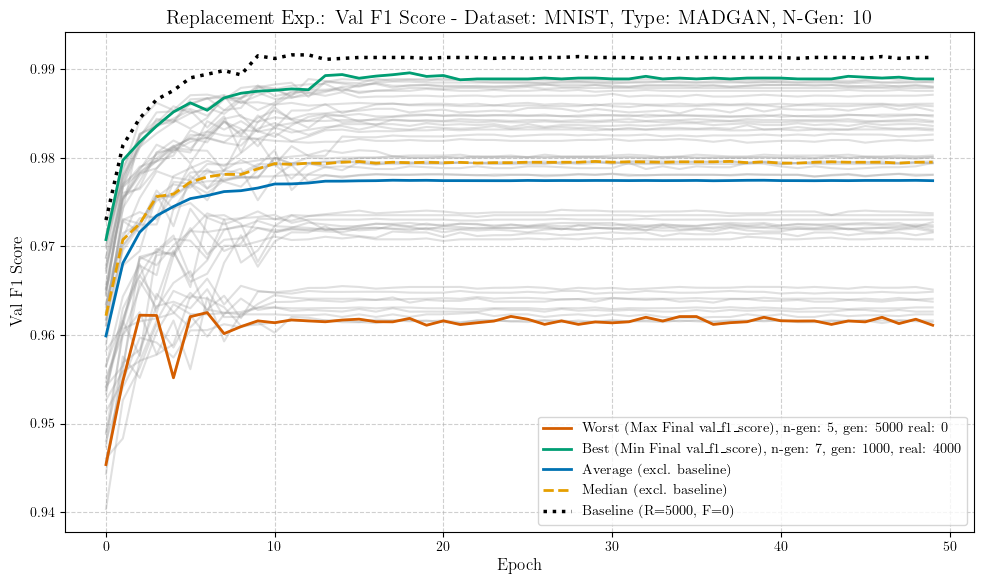
\includegraphics[width=\textwidth]{abb/strat_classifier_performance/MNIST_STRATIFIED_CLASSIFIERS_MADGAN_NEW/replacement_experiments/val_f1_score_MADGAN_MNIST_n_gen_10_all.png}
		\caption{F1 Score on MNIST over 50 epochs. Augmentation technique: MADGAN (K=10)}
        \label{fig:res_replacement_mnist_tda_vs_madgan__madgan}
	\end{subfigure}
	\begin{subfigure}{.85\textwidth}
		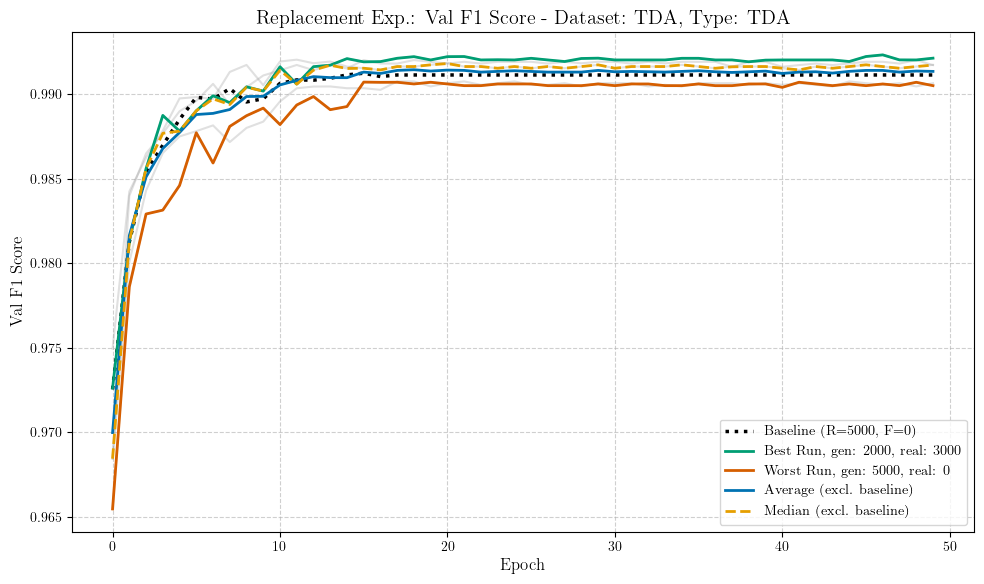
\includegraphics[width=\textwidth]{abb/strat_classifier_performance/tda_mnist/replacement_experiments/val_f1_score_tda_mnist_mnist_all.png}
		\caption{F1 Score on MNIST over 50 epochs. Augmentation Technique: TDA}
        \label{fig:res_replacement_mnist_tda_vs_madgan__tda}
	\end{subfigure}
%%%%%%%%%%%%%%
\end{figure}

\begin{table}[H]
	\vspace{-1.5em}
	\centering
	\begin{tabular}{|c|c|c|c|}
		\hline
		Run Type & Experiment & Val F1 \\ \hline
		best & \(G_{10, 7}\), R:4000, F:1000 & $0.9889$\\ \hline
		worst & \(G_{10, 5}\), R:0, F:5000 & $0.9611$\\ \hline
		median & G (K=10) & $0.9795$\\ \hline
		average & G (K=10) & $0.9774$
		\\ \hline
	\end{tabular}
    \caption{Final F1 Scores after 50 epochs. Augmentation technique: MADGAN}
        \label{tab:res_replacement_mnist_tda_vs_madgan__madgan}
\end{table}
\begin{table}[H]
	\centering
	\vspace{-1.5em}
	\begin{tabular}{|c|c|c|c|c|}
		\hline
		Run Type & Metric & Performance \\ \hline
		best & TDA (R:3000, F:2000) & $0.9922$\\ \hline
		worst & TDA (R:0, F:5000) & $0.9905$\\ \hline
		median & TDA & $0.9917$\\ \hline
		average & TDA & $0.9914$
		\\ \hline
	\end{tabular}
    \caption{Final F1 Scores after 50 epochs. Augmentation technique: TDA}
        \label{tab:res_replacement_mnist_tda_vs_madgan__tda}
\end{table}

The results for TDA, shown in figure \ref{fig:res_replacement_mnist_tda_vs_madgan__tda} and summarized in table \ref{tab:res_replacement_mnist_tda_vs_madgan__tda}. The graphs in the corresponding figure show all out rapid convergence and a stable training over the $50$ epochs. With a small spread of the results, all replacement ratios \\\(\left[ (R:5000, F:0), ..., (R:0, F:5000) \right]\) consistently result in excellent performance with an average F1 score of $0.9914$. The best and worst results are close to the average and both are over $0.99$, only differing in the third decimals. This leads to the conclusion that replacing training images for a classifier with modified images via traditional methods had minimal negative impact on the classifiers' performance, measured on the validation set via the F1 score. It is to point out, that the best, average and median performance surpassed the baseline allowing the conclusion that the replacement of real images with their augmented counterpart had a positive impact on average.

The performance using GDA with samples form MADGAN (K=10) model is presented in Figure \ref{fig:res_replacement_mnist_tda_vs_madgan__madgan} and Table \ref{tab:res_replacement_mnist_tda_vs_madgan__madgan}. It is important to note again, that the figure and the summary statistics encompass results across the 10 individual generators and across all replacement ratios resulting in a total of $60$ total classifiers. The graph shows convergence to a slightly lower F1 scores, compared to those from TDA. Here, the conclusion can be drawn that the replacement of real with augmented images resulted in an overall negative impact. The summary table quantifies this fact: the average final F1 score across ratios and generators is $0.9775$, which is significantly lower than the average of the traditional augmentation. While the best setup (\(G_{10,7}, R:4000, F:1000\)) reached a good score: $0.9889$; it is lower than the average performance across the different ratios in the TDA experiment. Even the worst performing classifier in the TDA experiment is better than the best score for GDA in this case.

In direct comparison, the TDA consistently outperforms GDA (with its best resulting setting, MADGAN (K=10)) in this replacement scenario. Replacing the real data with synthetic lead to a noticeable degradation of the classifiers' performance on the validation set. Taking the results from question 1 into account (\ref{exp_results_ans_q1}), even the MADGAN setup resulting in the best FID score are not as effective as traditional augmented real data, when substituting the real samples in the training set.

\newpage
\noindent\textbf{Expansion Experiment, Dataset: MNIST}
\begin{figure}[H]
	\centering
	\begin{subfigure}{.85\textwidth}
		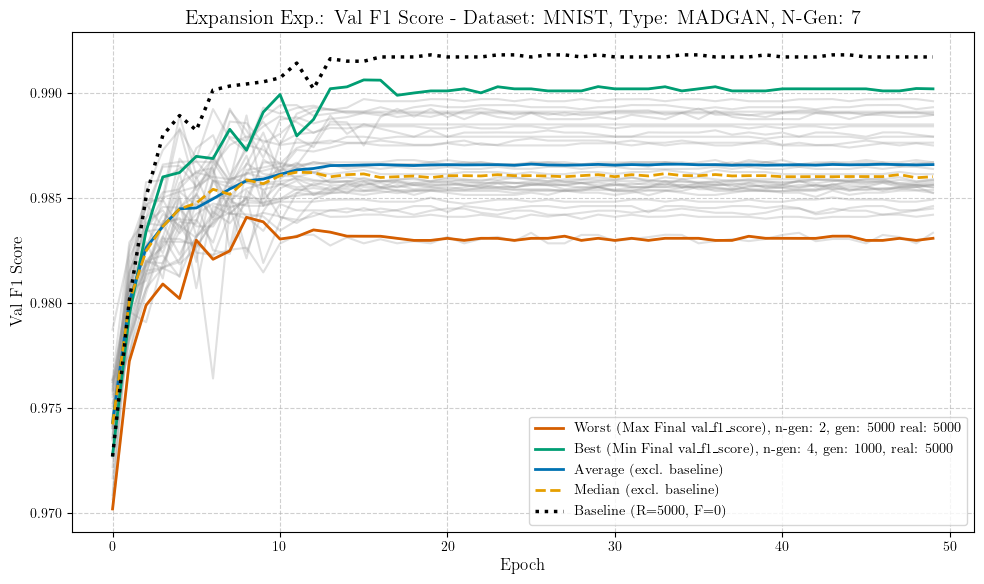
\includegraphics[width=\textwidth]{abb/strat_classifier_performance/MNIST_STRATIFIED_CLASSIFIERS_MADGAN_NEW/expansion_experiments/val_f1_score_MADGAN_MNIST_n_gen_7_all.png}
		\caption{F1 Score on MNIST over 50 epochs. Augmentation technique: MADGAN (K=7)}
        \label{fig:res_expansion_mnist_tda_vs_madgan__madgan}
	\end{subfigure}
	\begin{subfigure}{.85\textwidth}
		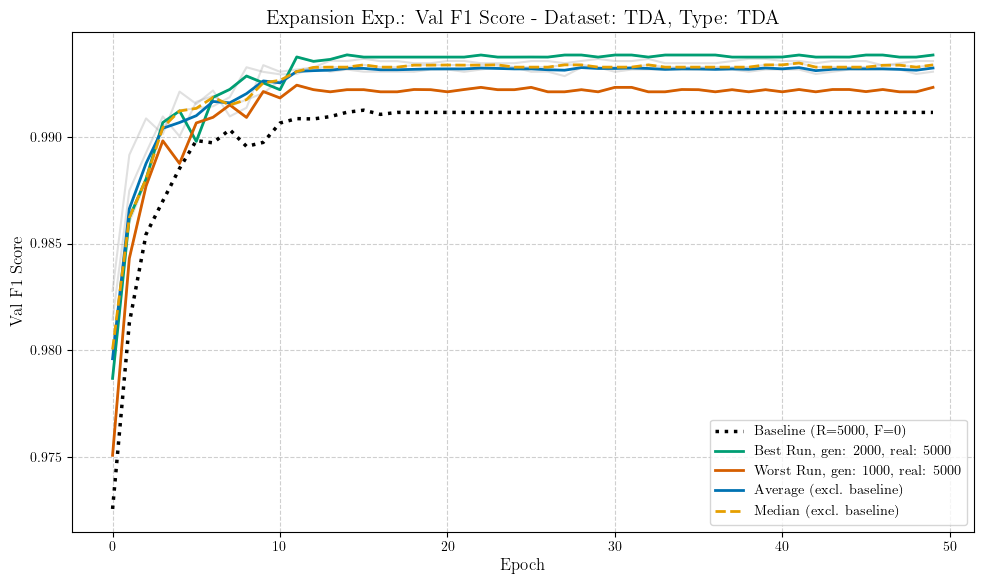
\includegraphics[width=\textwidth]{abb/strat_classifier_performance/tda_mnist/expansion_experiments/val_f1_score_tda_mnist_mnist_all.png}
		\caption{F1 Score on MNIST over 50 epochs. Augmentation Technique: TDA}
        \label{fig:res_expansion_mnist_tda_vs_madgan__tda}
	\end{subfigure}
%%%%%%%%%%%%%%
\end{figure}

\begin{table}[H]
	\vspace{-1.5em}
	\centering
	\begin{tabular}{|c|c|c|c|}
		\hline
		Run Type & Experiment & Val F1 \\ \hline
		best & \(G_{7, 4}\), R:5000, F:1000 & $0.9902$\\ \hline
		worst & \(G_{7, 2}\), R:5000, F:5000 & $0.9831$\\ \hline
		median & G (K=7) & $0.9860$\\ \hline
		average & G (K=7) & $0.9866$
		\\ \hline
	\end{tabular}
    \caption{Final F1 Scores after 50 epochs. Augmentation technique: MADGAN}
        \label{tab:res_expansion_mnist_tda_vs_madgan__madgan}
\end{table}
\begin{table}[H]
	\centering
	\vspace{-1.5em}
	\begin{tabular}{|c|c|c|c|c|}
		\hline
		Run Type & Experiment & Performance \\ \hline
		best & TDA (R:5000, F:2000) & $0.9938$\\ \hline
		worst & TDA (R:5000, F: 1000) & $0.9923$\\ \hline
		median & TDA & $0.9934$\\ \hline
		average & TDA & $0.9932$
		\\ \hline
	\end{tabular}
    \caption{Final F1 Scores after 50 epochs. Augmentation technique: TDA}
        \label{tab:res_expansion_mnist_tda_vs_madgan__tda}
\end{table}

The results using TDA (Table \ref{tab:res_expansion_mnist_tda_vs_madgan__tda}) show consistently high performance. The average final F1 score across all expansion levels (adding 0 to 5,000 augmented samples per class) is 0.9932, with minimal variation between the best (0.9938, achieved when adding 2,000 augmented samples) and worst (0.9923) cases. This indicates that expanding the dataset with traditionally augmented samples maintains, and perhaps very slightly improves, the already high baseline performance on MNIST.

In contrast, using GDA with samples generated by the MADGAN (K=7) model did not yield performance improvements over the baseline trained only on real data. To be noted explicitly, none of the expansion experiments using MADGAN GDA surpassed the baseline performance level (see: \ref{app_strat_class_performance_madgan_mnist}). The summary statistics in Table \ref{tab:res_expansion_mnist_tda_vs_madgan__madgan}, which cover results across all 7 generators and all expansion ratios, confirm this. The average final F1 score is 0.9866, noticeably lower than the TDA results. The best-performing run across all generators and expansion levels only reached 0.9902 (using generator \(G_{7,4}\) when adding 1,000 synthetic samples), which is below even the worst TDA result. Performance tended to decrease as more synthetic data was added, with the lowest score (0.9831) occurring when the maximum of 5,000 synthetic samples per class were added (using generator \(G_{7,2}\)).

Comparing the two augmentation strategies in the expansion scenario, TDA is clearly superior on MNIST in this setup. Expanding the dataset with traditionally augmented data maintains excellent performance, whereas expanding with MADGAN-generated synthetic data fails to improve over the real-data baseline and leads to lower overall performance. This suggests that the synthetic samples from MADGAN (K=7), despite the model potentially having good generative scores, dilute rather than enhance the training data quality when added to the real MNIST dataset for this downstream classification task.


\newpage
\noindent\textbf{Replacement Experiment, Dataset: Fashion-MNIST}
\begin{figure}[H]
	\centering
	\begin{subfigure}{.85\textwidth}
		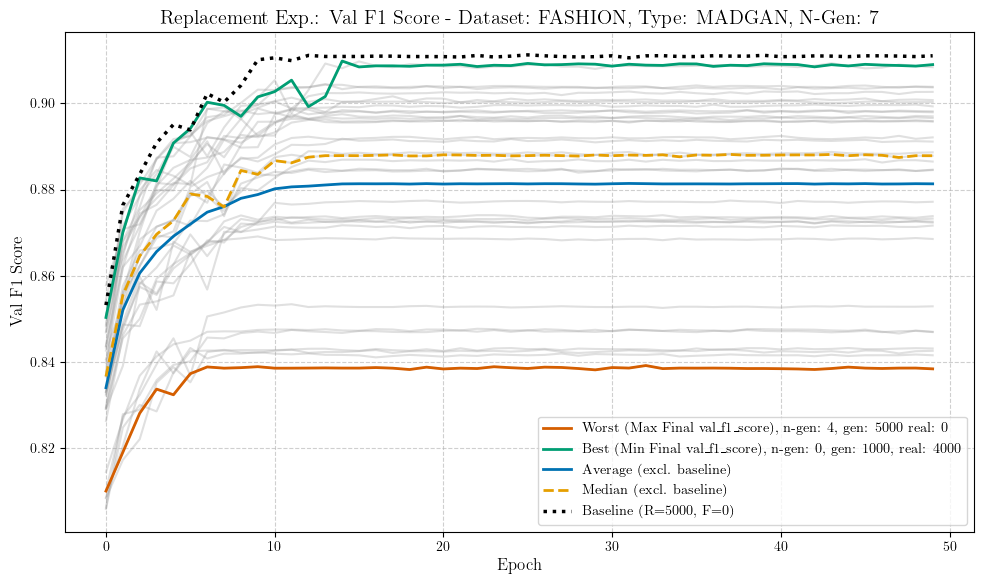
\includegraphics[width=\textwidth]{abb/strat_classifier_performance/FASHION_STRATIFIED_CLASSIFIERS_MADGAN_NEW/replacement_experiments/val_f1_score_MADGAN_FASHION_n_gen_7_all.png}
		\caption{F1 Score on FASHION over 50 epochs. Augmentation tech.: MADGAN (K=7)}
        \label{fig:res_replacement_fashion_tda_vs_madgan__madgan}
	\end{subfigure}
	\begin{subfigure}{.85\textwidth}
		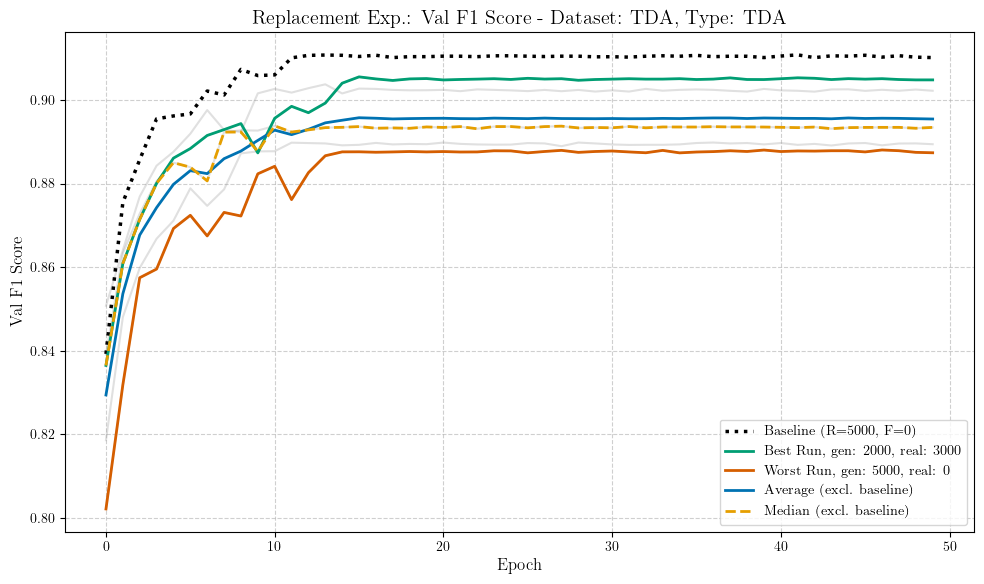
\includegraphics[width=\textwidth]{abb/strat_classifier_performance/tda_fashion_mnist/replacement_experiments/val_f1_score_tda_fashion_mnist_fashion_all.png}
		\caption{F1 Score on FASHION over 50 epochs. Augmentation Technique: TDA}
        \label{fig:res_replacement_fashion_tda_vs_madgan__tda}
	\end{subfigure}
%%%%%%%%%%%%%%
\end{figure}

\begin{table}[H]
	\vspace{-1.5em}
	\centering
	\begin{tabular}{|c|c|c|c|}
		\hline
		Run Type & Experiment & Val F1 \\ \hline
		best & \(G_{7, 2}\), R:4000, F:1000 & $0.9079$\\ \hline
		worst & \(G_{7, 0}\), R:0, F:5000 & $0.3419$\\ \hline
		median & G (K=7) & $0.8927$\\ \hline
		average & G (K=7) & $0.7993$
		\\ \hline
	\end{tabular}
    \caption{Final F1 Scores after 50 epochs. Augmentation tech.: MADGAN (K=7)}
        \label{tab:res_replacement_fashion_tda_vs_madgan__madgan}
\end{table}
\begin{table}[H]
	\centering
	\vspace{-1.5em}
	\begin{tabular}{|c|c|c|c|c|}
		\hline
		Run Type & Experiment & Val F1 \\ \hline
		best & TDA (R:3000, F:2000) & $0.9048$\\ \hline
		worst & TDA (R:0, F:5000) & $0.8874$\\ \hline
		median & TDA & $0.8934$\\ \hline
		average & TDA & $0.8955$
		\\ \hline
	\end{tabular}
    \caption{Final F1 Scores after 50 epochs. Augmentation technique: TDA}
        \label{tab:res_replacement_fashion_tda_vs_madgan__tda}
\end{table}
For TDA (Table \ref{tab:res_replacement_fashion_tda_vs_madgan__tda}), the results indicate reasonably strong and relatively stable classifier performance as real data is replaced by traditionally augmented samples. The average final F1 score across all replacement ratios is 0.8955. Performance degrades moderately as more real data is substituted, with the best score (0.9048) observed at a mix of 3000 real and 2000 augmented samples per class, and the worst score (0.8874) occurring when using only augmented data (0 real, 5000 augmented). The overall range is narrow, suggesting TDA provides consistent results.

The MADGAN (K=7) GDA results (Table \ref{tab:res_replacement_fashion_tda_vs_madgan__madgan}) reveal a much higher degree of variability. These summary statistics encompass results across all 7 individual generators and all replacement ratios. Notably, the best-performing run (generator \(G_{7,2}\) with 4000 real / 1000 fake samples) achieved an F1 score of 0.9079, slightly surpassing the best TDA result. However, extreme inconsistency offsets this potential advantage. The worst-performing run (generator \(G_{7,0}\) using only synthetic data) yielded a drastically low F1 score of 0.3419, far below the worst TDA score. This disparity heavily impacts the average F1 score for MADGAN GDA, bringing it down to 0.7993, significantly lower than the TDA average. Interestingly, the median F1 score for MADGAN GDA (0.8927) is quite close to the TDA median (0.8934), suggesting that while the average is poor due to outliers, typical performance might be closer to TDA.

In direct comparison for the replacement scenario on Fashion-MNIST, TDA offers more reliable and consistent performance. While MADGAN GDA demonstrates the potential to slightly exceed TDA's peak performance under specific optimal conditions (best generator, limited replacement), it suffers from extreme variability. Relying solely on synthetic data from weaker generators leads to a catastrophic performance drop, making MADGAN GDA a much less robust strategy on average compared to TDA when replacing real data in this setup.


\newpage
\noindent\textbf{Expansion Experiment, Dataset: Fashion-MNIST}
\begin{figure}[H]
	\centering
	\begin{subfigure}{.85\textwidth}
		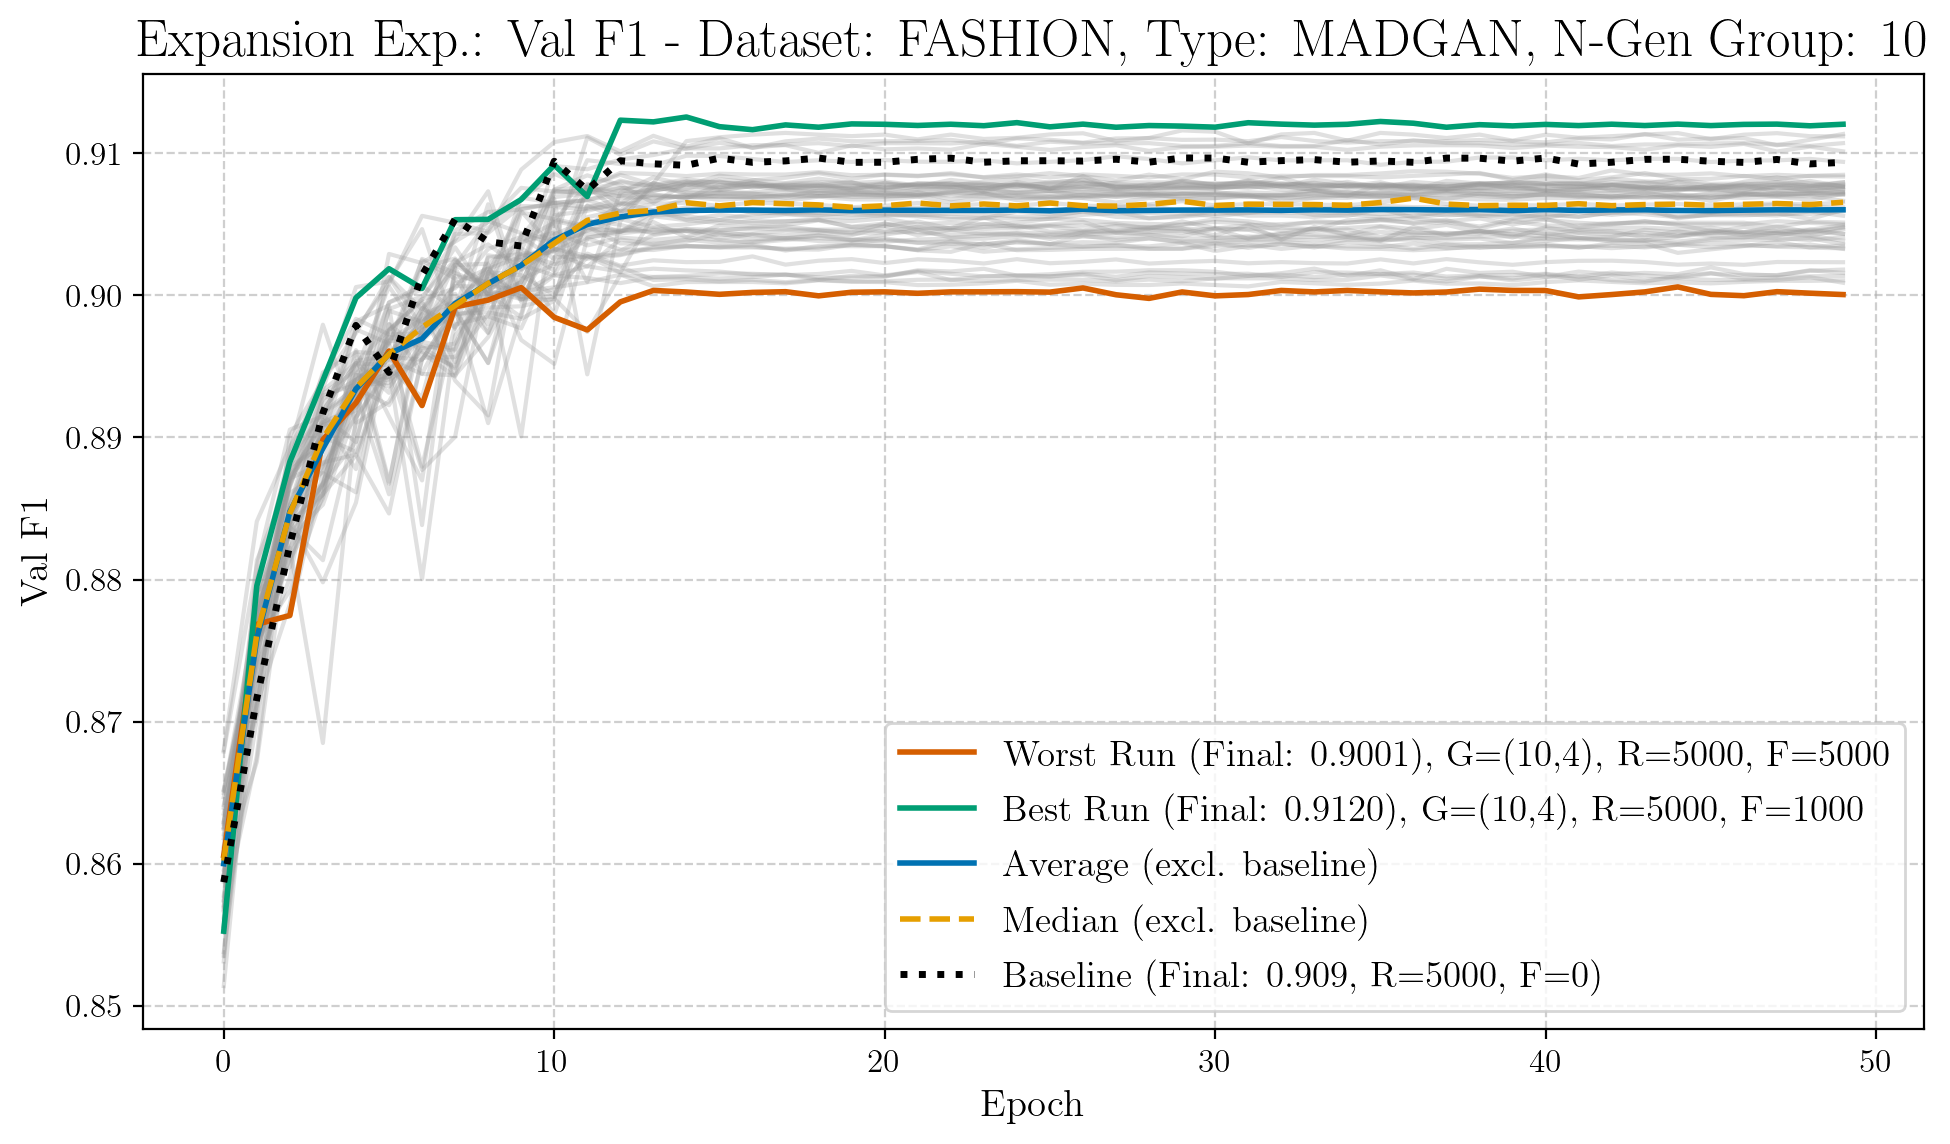
\includegraphics[width=\textwidth]{abb/strat_classifier_performance/FASHION_STRATIFIED_CLASSIFIERS_MADGAN_NEW/expansion_experiments/val_f1_score_MADGAN_FASHION_n_gen_10_all.png}
		\caption{F1 Score on FASHION over 50 epochs. Augmentation tech.: MADGAN (K=10)}
        \label{fig:res_expansion_fashion_tda_vs_madgan__madgan}
	\end{subfigure}
	\begin{subfigure}{.85\textwidth}
		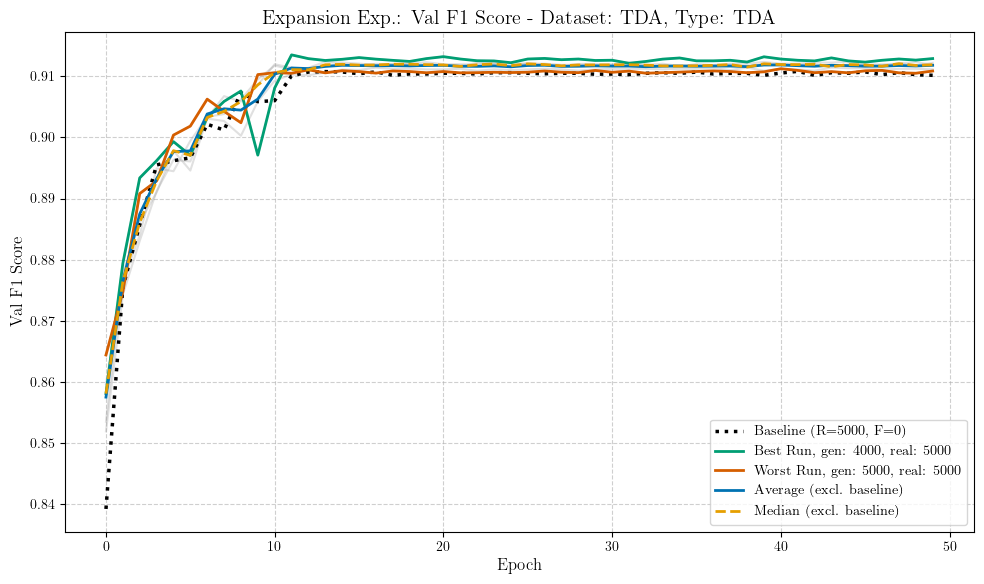
\includegraphics[width=\textwidth]{abb/strat_classifier_performance/tda_fashion_mnist/expansion_experiments/val_f1_score_tda_fashion_mnist_fashion_all.png}
		\caption{F1 Score on FASHION over 50 epochs. Augmentation Technique: TDA}
        \label{fig:res_expansion_fashion_tda_vs_madgan__tda}
	\end{subfigure}
%%%%%%%%%%%%%%
\end{figure}

\begin{table}[H]
	\vspace{-1.5em}
	\centering
	\begin{tabular}{|c|c|c|c|}
		\hline
		Run Type & Experiment & Val F1 \\ \hline
		best & \(G_{10, 4}\), R:5000, F:1000 & $0.9120$\\ \hline
		worst & \(G_{10, 4}\), R:5000, F:5000 & $0.9001$\\ \hline
		median & G (K=10) & $0.9066$\\ \hline
		average & (K=10) & $0.9060$
		\\ \hline
	\end{tabular}
    \caption{Final F1 Scores after 50 epochs. Augmentation tech.: MADGAN (K=10)}
        \label{tab:res_expansion_fashion_tda_vs_madgan__madgan}
\end{table}
\begin{table}[H]
	\centering
	\vspace{-1.5em}
	\begin{tabular}{|c|c|c|c|c|}
		\hline
		Run Type & Experiment & Val F1 \\ \hline
		best & TDA (R:5000, F:4000) & $0.9129$\\ \hline
		worst & TDA (R:5000, F:5000) & $0.9108$\\ \hline
		median & TDA & $0.9119$\\ \hline
		average & TDA & $0.9118$
		\\ \hline
	\end{tabular}
    \caption{Final F1 Scores after 50 epochs. Augmentation technique: TDA}
        \label{tab:res_expansion_fashion_tda_vs_madgan__tda}
\end{table}

Above results show, that data expansion on Fashion-MNIST is beneficial for both augmentation techniques. Unlike observations on MNIST, for which MADGAN GDA did not surpass the respective baseline. Utilizing TDA (Table \ref{tab:res_expansion_fashion_tda_vs_madgan__tda}) to add samples improves the classifiers performance over the baseline, achieving a peak F1 score of $0.9129$ when adding $4.000$ augmented samples to each class. The F1 performance remains high, despite varying ratios or real to fake images. The setting achieved an average F1 score of $0.9118$ and even the worst case (adding $5.000$ samples) scored $0.9108$.

On the Fashion-MNIST dataset, data expansion proved advantageous for both augmentation strategies, a notable contrast to earlier MNIST findings where MADGAN GDA struggled to exceed baseline performance. With Traditional Data Augmentation (TDA), as detailed in \ref{tab:res_expansion_fashion_tda_vs_madgan__tda}, incorporating additional augmented samples demonstrably boosted classifier F1 scores over the R:5000/F:0 baseline. This enhancement culminated in a peak F1 score of $0.9129$ with the addition of $4.000$ augmented samples per class. TDA maintained remarkably high and stable performance throughout the expansion, evidenced by an average F1 score of $0.9118$ and a strong worst-case score of $0.9108$ even when $5.000$ augmented samples were added.

Generative Data Augmentation using MADGAN (K=10) also improved performance over the presumed baseline, as indicated by the summary statistics in \ref{tab:res_expansion_fashion_tda_vs_madgan__madgan}. Its best-case F1 score reached $0.9120$, achieved by generator \(G_{10,4}\) with an addition of $1.000$ synthetic samples per class, closely rivaling TDA's peak and underscoring GDA's effectiveness in this scenario. While this peak is promising, MADGAN GDA exhibited slightly less consistency than TDA. Its average F1 score ($0.9060$) and median ($0.9066$) were marginally lower than TDA's equivalents. Furthermore, performance showed a more pronounced decline when maximally expanded with $5.000$ synthetic samples, dropping to $0.9001$ in the worst run—a score notably below TDA's worst case. Nevertheless, the variability across MADGAN's generators and expansion ratios was considerably less extreme than what was observed in the Fashion-MNIST replacement experiments.

Ultimately, for data expansion on Fashion-MNIST, both TDA and MADGAN GDA (K=10) offered tangible benefits over relying solely on the original real data. TDA, however, maintained a slight overall advantage, delivering marginally higher peak performance ($0.9129$ for TDA vs. $0.9120$ for MADGAN GDA) and superior stability, particularly evident when large volumes of augmented data were incorporated. While MADGAN GDA proved highly competitive by nearly matching TDA's peak, its slightly lower average scores and more significant performance drop under maximum expansion conditions indicate that TDA remains the more robust expansion technique in this specific setup, though MADGAN GDA is clearly a viable alternative.


\newpage
\subsubsection[Question 3]{MADGAN GDA vs. Deep Convolutional/Conditional GAN GDA} \label{exp_results_ans_q3}
In the foregoing chapter (\ref{exp_results_ans_q2}), the most successful setting for the MADGAN architecture has been set. MADGAN with K=10 for Replacement-, with K=7 for the Expansion scenario on MNIST and for Fashion-MNIST K=7 for Replacement- and K=10 for Expansion proved to perform best under given circumstances. Following, the same settings for the respective dataset and the corresponding experimental setup (replacement, expansion) will be used to compare against the best performing architecture of deep convolutional and conditional GANs. For both, the Replacement and Expansion scenario, the cGAN surpassed the performance of the DCGAN. Thus, the cGAN is selected for direct comparison. The DCGAN will only be described and linked were fit.

TODO: preamble the results of the following experiments
\newpage

\noindent\textbf{Replacement Experiment, Dataset: MNIST}
\begin{figure}[H]
	\centering
	\begin{subfigure}{.85\textwidth}
		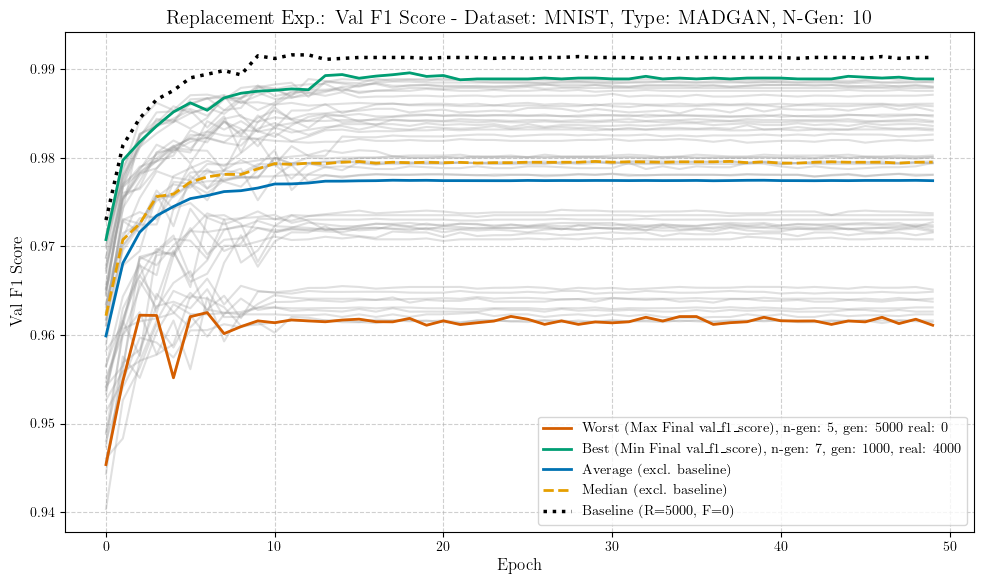
\includegraphics[width=\textwidth]{abb/strat_classifier_performance/MNIST_STRATIFIED_CLASSIFIERS_MADGAN_NEW/replacement_experiments/val_f1_score_MADGAN_MNIST_n_gen_10_all.png}
		\caption{F1 Score on MNIST over 50 epochs. Augmentation technique: MADGAN (K=10)}
        \label{fig:res_replacement_mnist_ccgan_vs_madgan__madgan}
	\end{subfigure}
	\begin{subfigure}{.85\textwidth}
		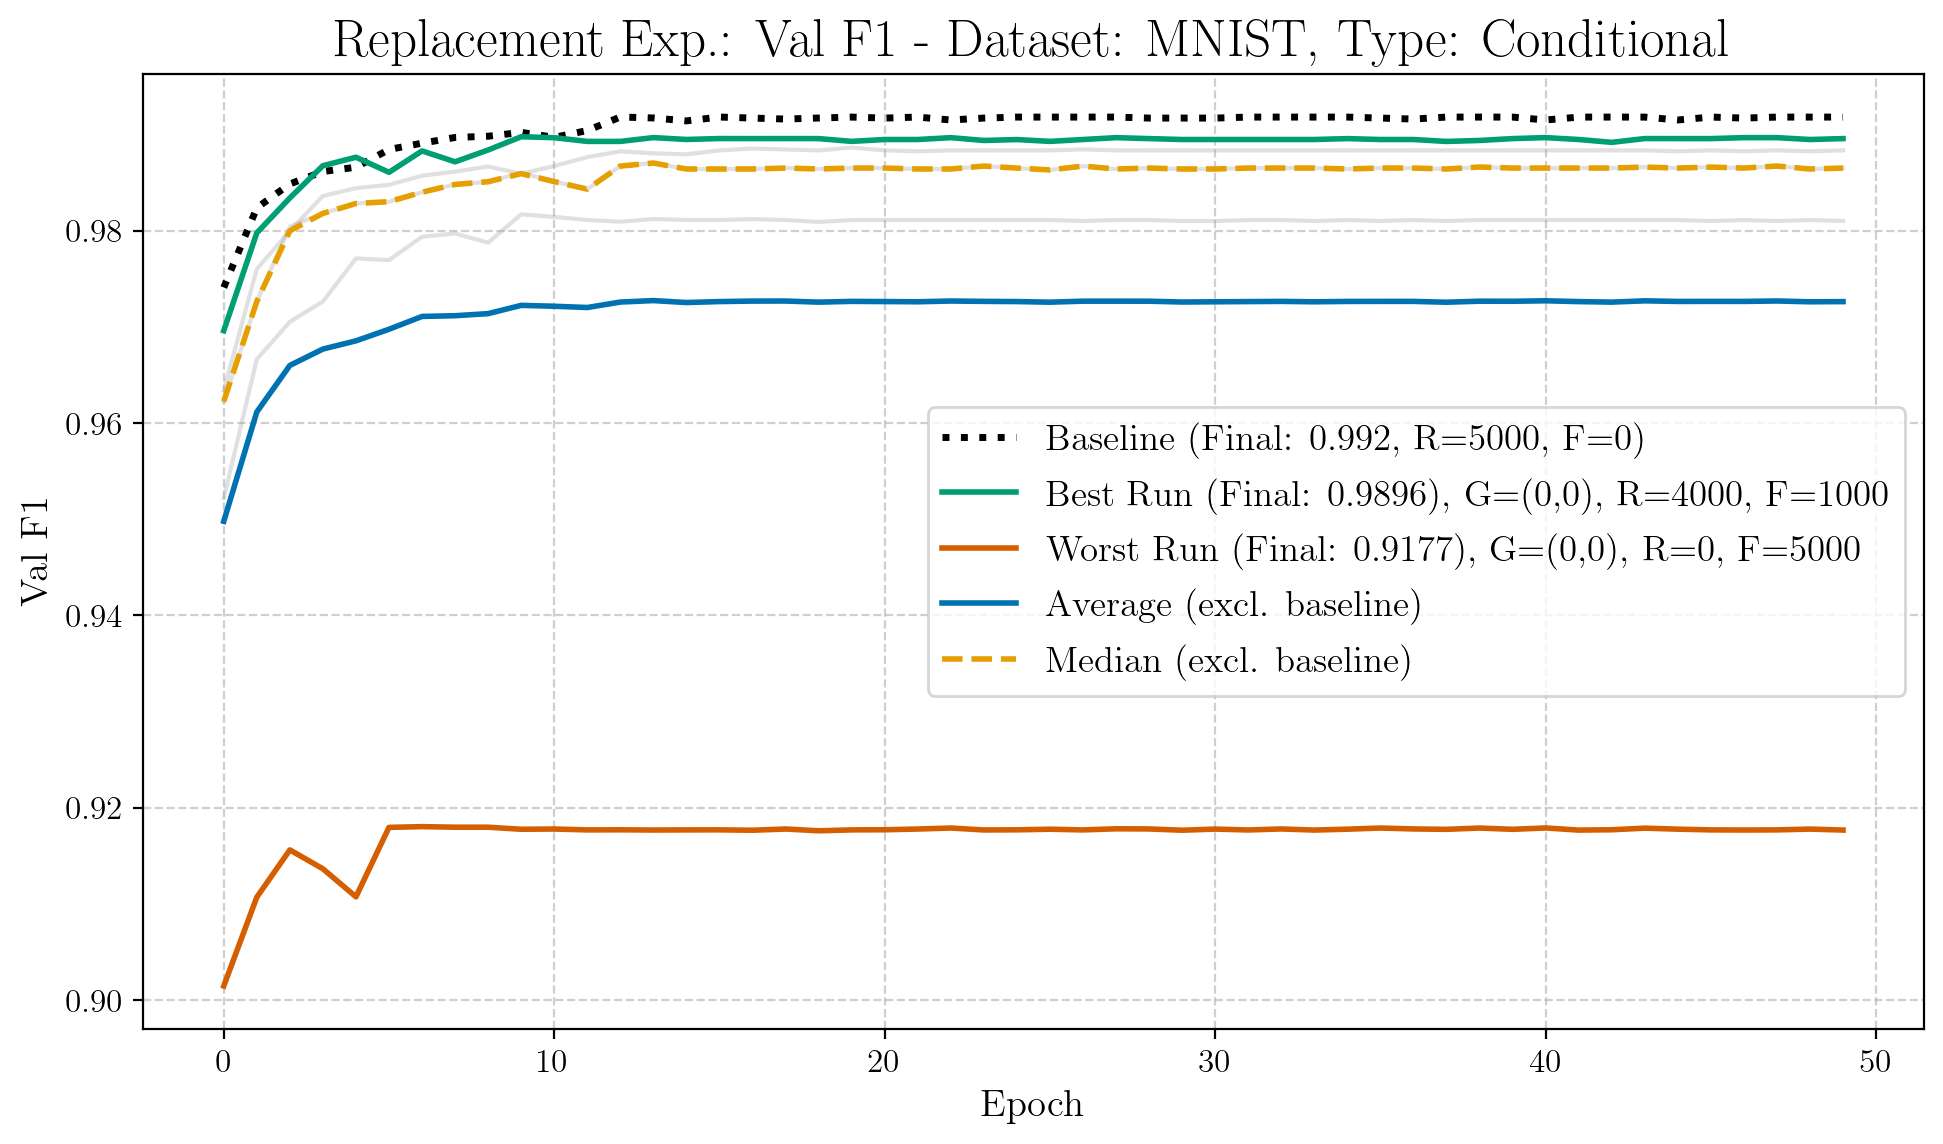
\includegraphics[width=\textwidth]{abb/strat_classifier_performance/MNIST_STRATIFIED_CLASSIFIERS_COND_GAN/replacement_experiments/val_f1_score_['COND']_MNIST_all.png}
		\caption{F1 Score on MNIST over 50 epochs. Augmentation Technique: cGAN}
        \label{fig:res_replacement_mnist_ccgan_vs_madgan__cgan}
	\end{subfigure}
%%%%%%%%%%%%%%
\end{figure}

\begin{table}[H]
	\vspace{-1.5em}
	\centering
	\begin{tabular}{|c|c|c|c|}
		\hline
		Run Type & Experiment & Val F1 \\ \hline
		best & \(G_{10, 7}\), R:4000, F:1000 & $0.9889$\\ \hline
		worst & \(G_{10, 5}\), R:0, F:5000 & $0.9611$\\ \hline
		median & G (K=10) & $0.9795$\\ \hline
		average & G (K=10) & $0.9774$
		\\ \hline
	\end{tabular}
    \caption{Final F1 Scores after 50 epochs. Augmentation technique: MADGAN (K=10)}
        \label{tab:res_replacement_mnist_ccgan_vs_madgan__madgan}
\end{table}
\begin{table}[H]
	\centering
	\vspace{-1.5em}
	\begin{tabular}{|c|c|c|c|c|}
		\hline
		Run Type & Experiment & Val F1 \\ \hline
		best & Conditional (R:4000, F:1000) & $0.9896$\\ \hline
		worst & Conditional (R:0, F:5000) & $0.9177$\\ \hline
		median & Conditional & $0.9865$\\ \hline
		average & Conditional & $0.9726$
		\\ \hline
	\end{tabular}
    \caption{Final F1 Scores after 50 epochs. Augmentation technique: cGAN}
        \label{tab:res_replacement_mnist_ccgan_vs_madgan__cgan}
\end{table}
Both MADGAN (K=10) and cGAN demonstrate strong peak performance when replacing only a small amount of real data. As shown in Tables \ref{tab:res_replacement_mnist_ccgan_vs_madgan__madgan} and \ref{tab:res_replacement_mnist_ccgan_vs_madgan__cgan}, the best F1 scores achieved are very similar, with cGAN reaching $0.9896$ and MADGAN K=10 reaching $0.9889$, both occurring when 1,000 real samples per class were replaced with synthetic ones (R:4000, F:1000).

However, the two methods exhibit different robustness levels as more real data is replaced. The cGAN performance degrades significantly when relying entirely on synthetic data (R:0, F:5000), with the F1 score dropping to $0.9177$. In contrast, the MADGAN (K=10) framework shows greater resilience in the purely synthetic scenario; even the worst-performing generator (\(G_{10,5}\)) at full replacement achieved an F1 score of $0.9611$, considerably higher than cGAN's worst score.

This difference in worst-case performance impacts the overall statistics. While cGAN achieves a higher median F1 score ($0.9865$) compared to MADGAN K=10 ($0.9795$), suggesting better typical performance across intermediate replacement ratios, MADGAN K=10 achieves a slightly higher average F1 score ($0.9774$ vs. $0.9726$ for cGAN). This is because MADGAN's performance does not drop as drastically as cGAN's in the full replacement scenario. Consequently, cGAN exhibits a larger overall performance range (spread of ~$0.072$) compared to MADGAN K=10 (spread of ~$0.028$) in this replacement experiment.

In conclusion, when replacing real MNIST data, both cGAN and MADGAN (K=10) GDA achieve similar high peak performance with limited replacement. However, MADGAN (K=10) demonstrates superior robustness when large amounts of real data are substituted, particularly in the scenario using only synthetic data. While cGAN performs slightly better across median replacement ratios, its sharp decline in the full synthetic setting makes MADGAN (K=10) appear more consistent overall in this specific replacement task, yielding a slightly better average F1 score.
\newpage
\noindent\textbf{Expansion Experiment, Dataset: MNIST}
\begin{figure}[H]
	\centering
	\begin{subfigure}{.85\textwidth}
		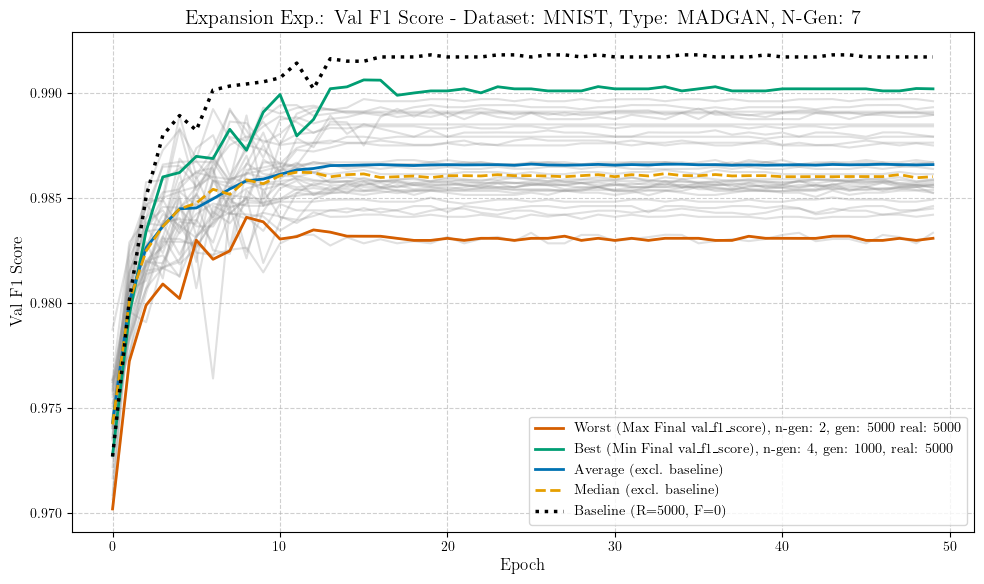
\includegraphics[width=\textwidth]{abb/strat_classifier_performance/MNIST_STRATIFIED_CLASSIFIERS_MADGAN_NEW/expansion_experiments/val_f1_score_MADGAN_MNIST_n_gen_7_all.png}
		\caption{F1 Score on MNIST over 50 epochs. Augmentation technique: MADGAN (K=7)}
        \label{fig:res_expansion_mnist_ccgan_vs_madgan__madgan}
	\end{subfigure}
	\begin{subfigure}{.85\textwidth}
		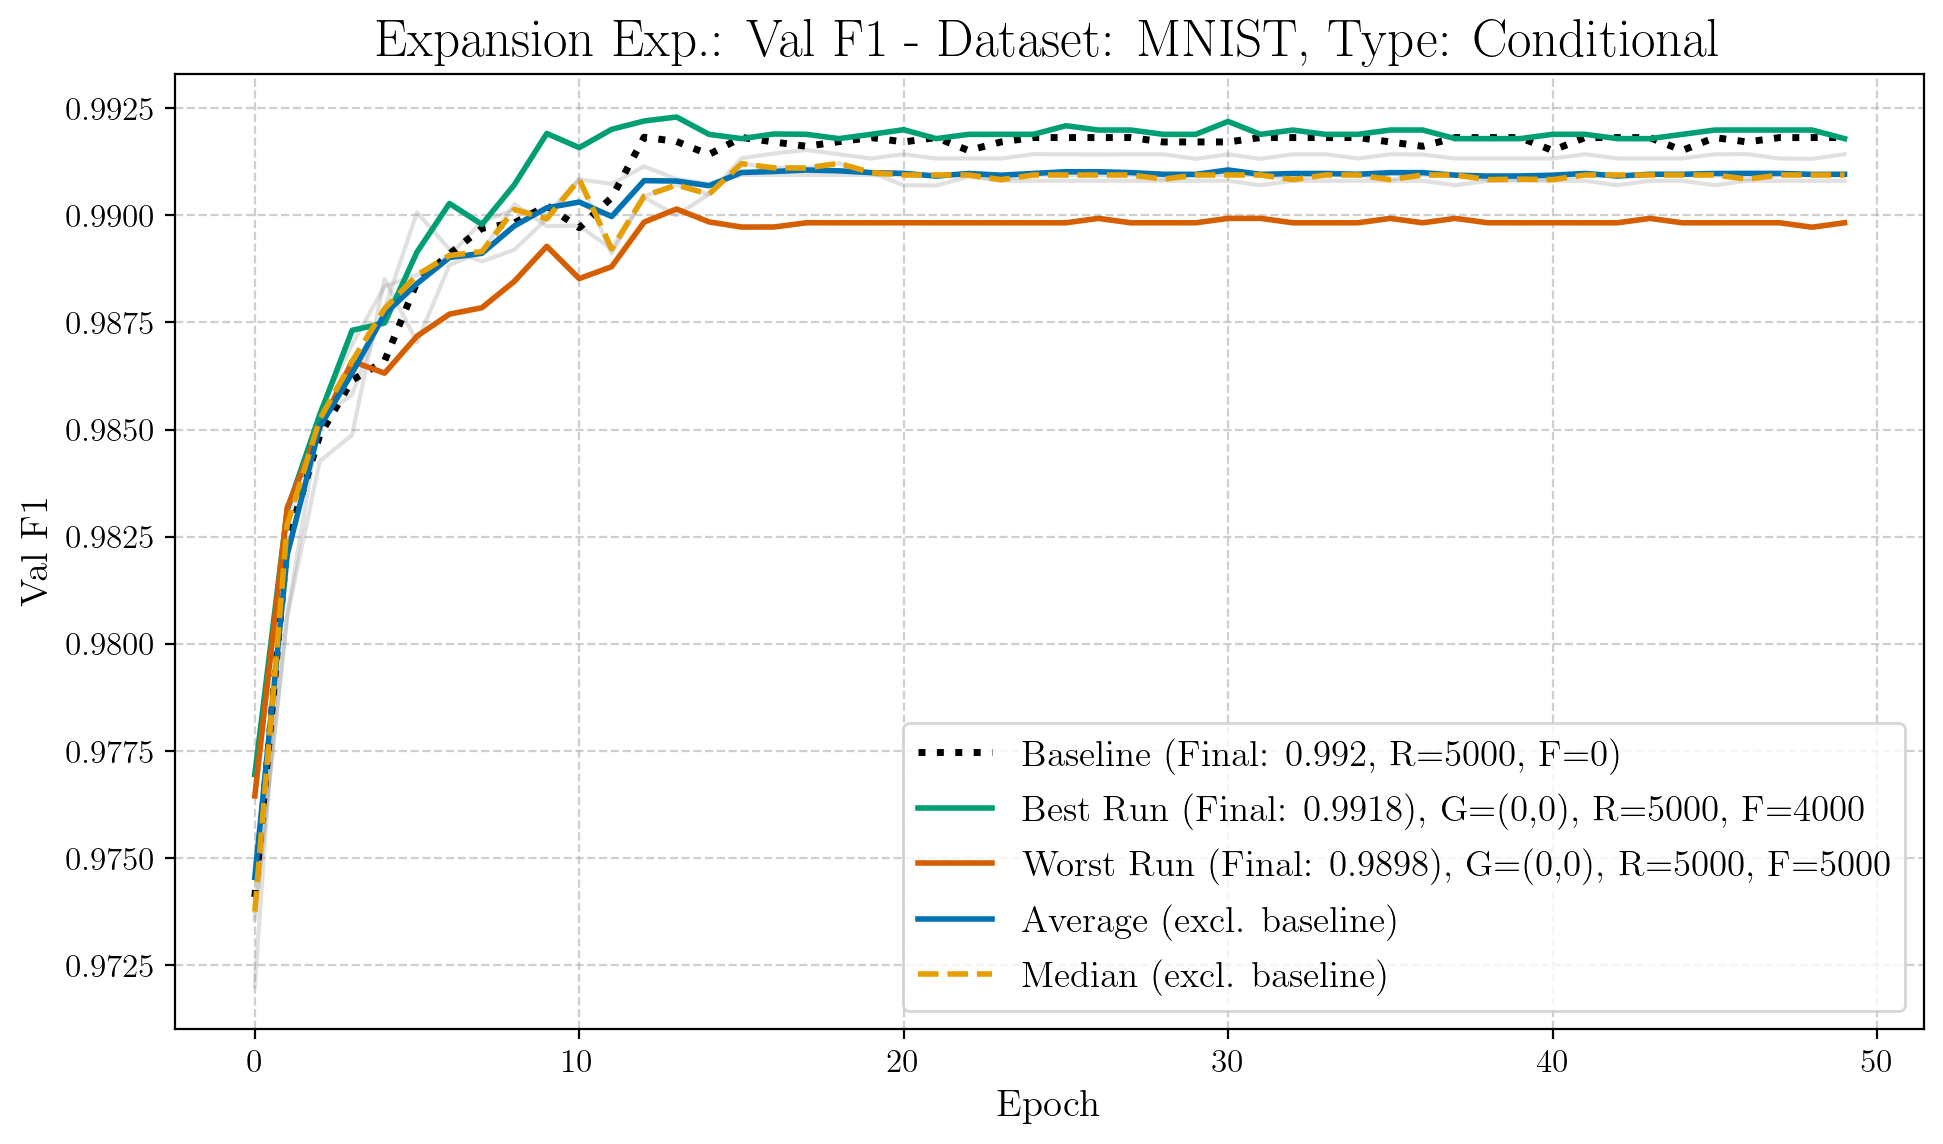
\includegraphics[width=\textwidth]{abb/strat_classifier_performance/MNIST_STRATIFIED_CLASSIFIERS_COND_GAN/expansion_experiments/val_f1_score_['COND']_MNIST_all.png}
		\caption{F1 Score on MNIST over 50 epochs. Augmentation Technique: cGAN}
        \label{fig:res_expansion_mnist_ccgan_vs_madgan__cgan}
	\end{subfigure}
%%%%%%%%%%%%%%
\end{figure}

\begin{table}[H]
	\vspace{-1.5em}
	\centering
	\begin{tabular}{|c|c|c|c|}
		\hline
		Run Type & Experiment & Val F1 \\ \hline
		best & \(G_{7, 4}\), R:5000, F:1000 & $0.9902$\\ \hline
		worst & \(G_{7, 2}\), R:5000, F:5000 & $0.9831$\\ \hline
		median & G (K=7) & $0.9860$\\ \hline
		average & G (K=7) & $0.9866$
		\\ \hline
	\end{tabular}
    \caption{Final F1 Scores after 50 epochs. Augmentation technique: MADGAN (K=10)}
        \label{tab:res_expansion_mnist_ccgan_vs_madgan__madgan}
\end{table}
\begin{table}[H]
	\centering
	\vspace{-1.5em}
	\begin{tabular}{|c|c|c|c|c|}
		\hline
		Run Type & Experiment & Val F1 \\ \hline
		best & Conditional (R:5000, F:4000) & $0.9918$\\ \hline
		worst & Conditional (R:5000, F:5000) & $0.9898$\\ \hline
		median & Conditional & $0.9909$\\ \hline
		average & Conditional & $0.9910$
		\\ \hline
	\end{tabular}
    \caption{Final F1 Scores after 50 epochs. Augmentation technique: cGAN}
        \label{tab:res_expansion_mnist_ccgan_vs_madgan__cgan}
\end{table}

The results clearly indicate that cGAN provides superior GDA performance compared to MADGAN (K=7) in this expansion scenario on MNIST. Examining the summary statistics, cGAN outperforms MADGAN K=7 across all metrics. The best F1 score achieved with cGAN ($0.9918$) is higher than MADGAN's best ($0.9902$). More significantly, cGAN maintains high performance even when the maximum number of synthetic samples are added (worst case F1 $0.9898$), whereas MADGAN's worst-case performance drops considerably lower ($0.9831$).

This difference in robustness is reflected in the average and median scores. cGAN achieves an average F1 of $0.9910$ and a median of $0.9909$, both higher than MADGAN's average (0.9866) and median ($0.9860$). Furthermore, cGAN exhibits much lower variability across the different expansion ratios compared to the variability observed across MADGAN's generators and expansion ratios (cGAN range ~$0.002$ vs. MADGAN range ~$0.007$).

Consistent with the earlier comparison against TDA, neither GDA method appears to significantly surpass their respective baseline performance achieved with $5.000$ real images per class alone. However, cGAN maintains performance very close to this baseline level, while adding MADGAN (K=7) samples tends to result in slightly lower F1 scores.

Interestingly, taking the performance of the DCGAN into account (\ref{app_STRAT_CLASS_PERF_mnist_DCGAN}), it is clear, that its peak performance is in line with the highest score of the best MADGAN setup (K=7). The difference in peak F1 score is only $0.0005$ ($0.9889 - 0.9884$). Furthermore, the spread of performance is significantly smaller for the DCGAN

In conclusion, for the task of expanding the MNIST training set, cGAN GDA is demonstrably more effective and stable than MADGAN (K=7) GDA. It achieves higher peak performance, maintains significantly better performance when large amounts of synthetic data are added, and exhibits less variability compared to the multi-generator approach in this configuration.

\newpage
\noindent\textbf{Replacement Experiment, Dataset: Fashion-MNIST}
\begin{figure}[H]
	\centering
	\begin{subfigure}{.85\textwidth}
		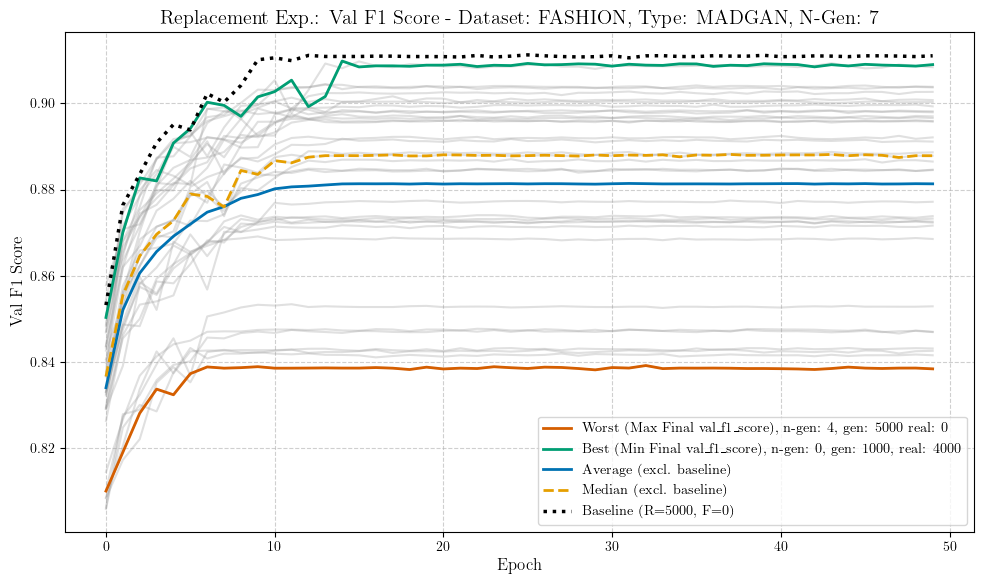
\includegraphics[width=\textwidth]{abb/strat_classifier_performance/FASHION_STRATIFIED_CLASSIFIERS_MADGAN_NEW/replacement_experiments/val_f1_score_MADGAN_FASHION_n_gen_7_all.png}
		\caption{F1 Score on FASHION over 50 epochs. Augmentation tech.: MADGAN (K=7)}
        \label{fig:res_replacement_fashion_cgan_vs_madgan__madgan}
	\end{subfigure}
	\begin{subfigure}{.85\textwidth}
		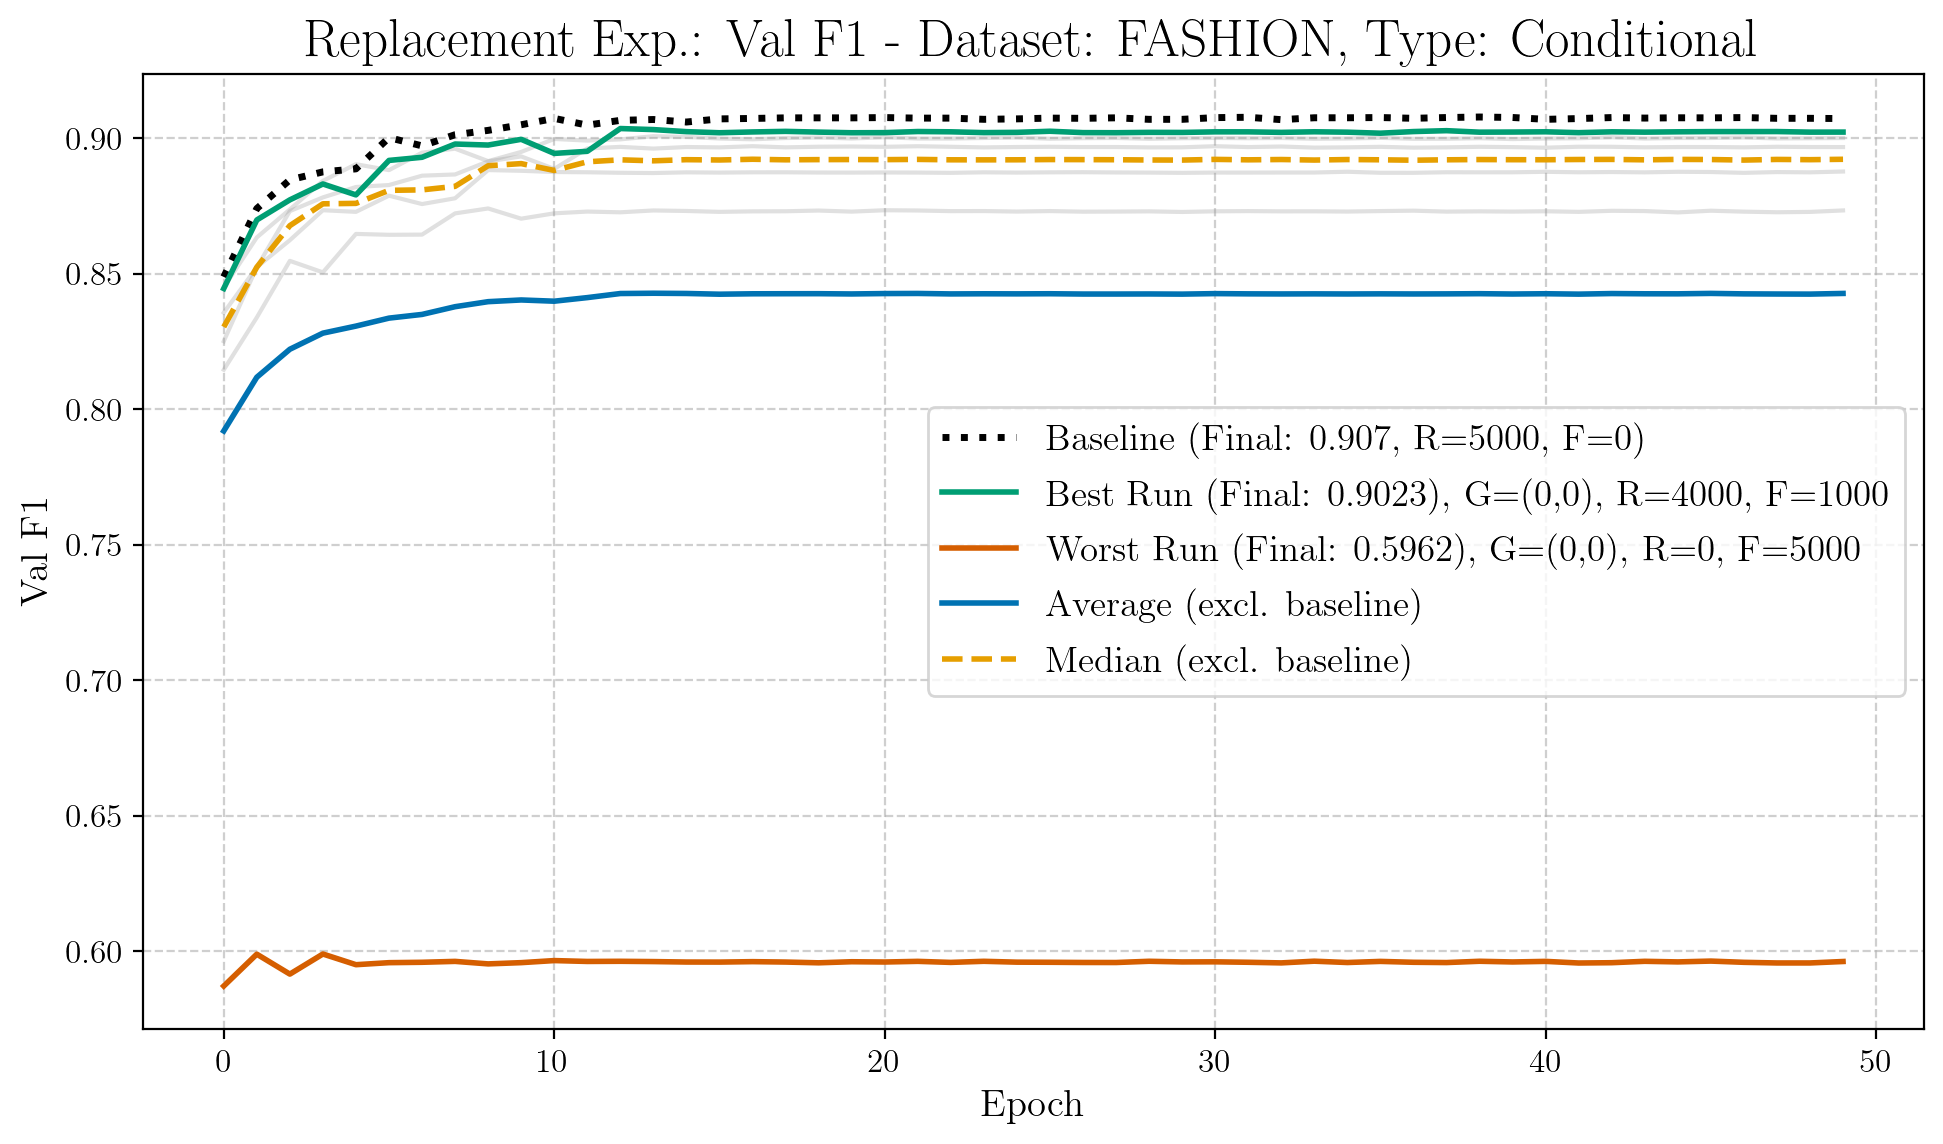
\includegraphics[width=\textwidth]{abb/strat_classifier_performance/FASHION_STRATIFIED_CLASSIFIERS_COND_GAN/replacement_experiments/val_f1_score_['COND']_FASHION_all.png}
		\caption{F1 Score on FASHION over 50 epochs. Augmentation Technique: cGAN}
        \label{fig:res_replacement_fashion_cgan_vs_madgan__cgan}
	\end{subfigure}
%%%%%%%%%%%%%%
\end{figure}

\begin{table}[H]
	\vspace{-1.5em}
	\centering
	\begin{tabular}{|c|c|c|c|}
		\hline
		Run Type & Experiment & Val F1 \\ \hline
		best & \(G_{7, 2}\), R:4000, F:1000 & $0.9079$\\ \hline
		worst & \(G_{7, 0}\), R:0, F:5000 & $0.3419$\\ \hline
		median & G = (K=7) & $0.8927$\\ \hline
		average & G = (K=7) & $0.7993$
		\\ \hline
	\end{tabular}
    \caption{Final F1 Scores after 50 epochs. Augmentation tech.: MADGAN (K=7)}
        \label{tab:res_replacement_fashion_cgan_vs_madgan__madgan}
\end{table}
\begin{table}[H]
	\centering
	\vspace{-1.5em}
	\begin{tabular}{|c|c|c|c|c|}
		\hline
		Run Type & Experiment & Val F1 \\ \hline
		best & Conditional (R:4000, F:1000) & $0.9023$\\ \hline
		worst & Conditional (R:0, F:5000) & $0.5962$\\ \hline
		median & Conditional & $0.8923$\\ \hline
		average & Conditional & $0.8427$
		\\ \hline
	\end{tabular}
    \caption{Final F1 Scores after 50 epochs. Augmentation technique: cGAN}
        \label{tab:res_replacement_fashion_cgan_vs_madgan__cgan}
\end{table}
Examining the peak performances, MADGAN (K=7) achieved a slightly higher best F1 score ($0.9079$ with generator \(G_{7,2}\) at R:4000, F:1000) compared to cGAN's best ($0.9023$ at the same replacement ratio). This suggests that, under optimal conditions (specific generator and limited replacement), MADGAN GDA can potentially offer a marginal advantage.

However, the performance when relying more heavily on synthetic data reveals significant differences in robustness. When all real data is replaced (R:0, F:5000), cGAN's F1 score drops to $0.5962$. While this is a substantial decrease, it is considerably better than the absolute worst-case for MADGAN (K=7), where using only synthetic data from its poorest performing generator (\(G_{7,0}\)) resulted in an F1 score of just $0.3419$.

This disparity in worst-case performance heavily influences the average scores. The cGAN achieves an average F1 score of $0.8427$ across all replacement ratios, which is notably higher than MADGAN K=7's average of $0.7993$. Interestingly, the median F1 scores are very similar ($0.8923$ for cGAN and 0.8927 for MADGAN K=7), indicating that the typical performance of both methods (excluding extreme outliers) is quite comparable. However, MADGAN (K=7) exhibits a much larger overall spread in performance (range ~$0.566$) compared to cGAN (range $~0.306$), primarily due to its extremely low worst-case scores.

In conclusion, for the replacement experiment on Fashion-MNIST, MADGAN (K=7) GDA can achieve a marginally higher peak F1 score than cGAN GDA with limited data replacement. However, cGAN demonstrates greater robustness on average and provides a significantly better worst-case performance when real data is fully substituted. The similar median scores suggest comparable typical performance, but MADGAN K=7 is less reliable overall due to the high variability among its individual generators, with some performing very poorly when used as the sole source of training data.

\newpage
\noindent\textbf{Expansion Experiment, Dataset: Fashion-MNIST}
\begin{figure}[H]
	\centering
	\begin{subfigure}{.85\textwidth}
		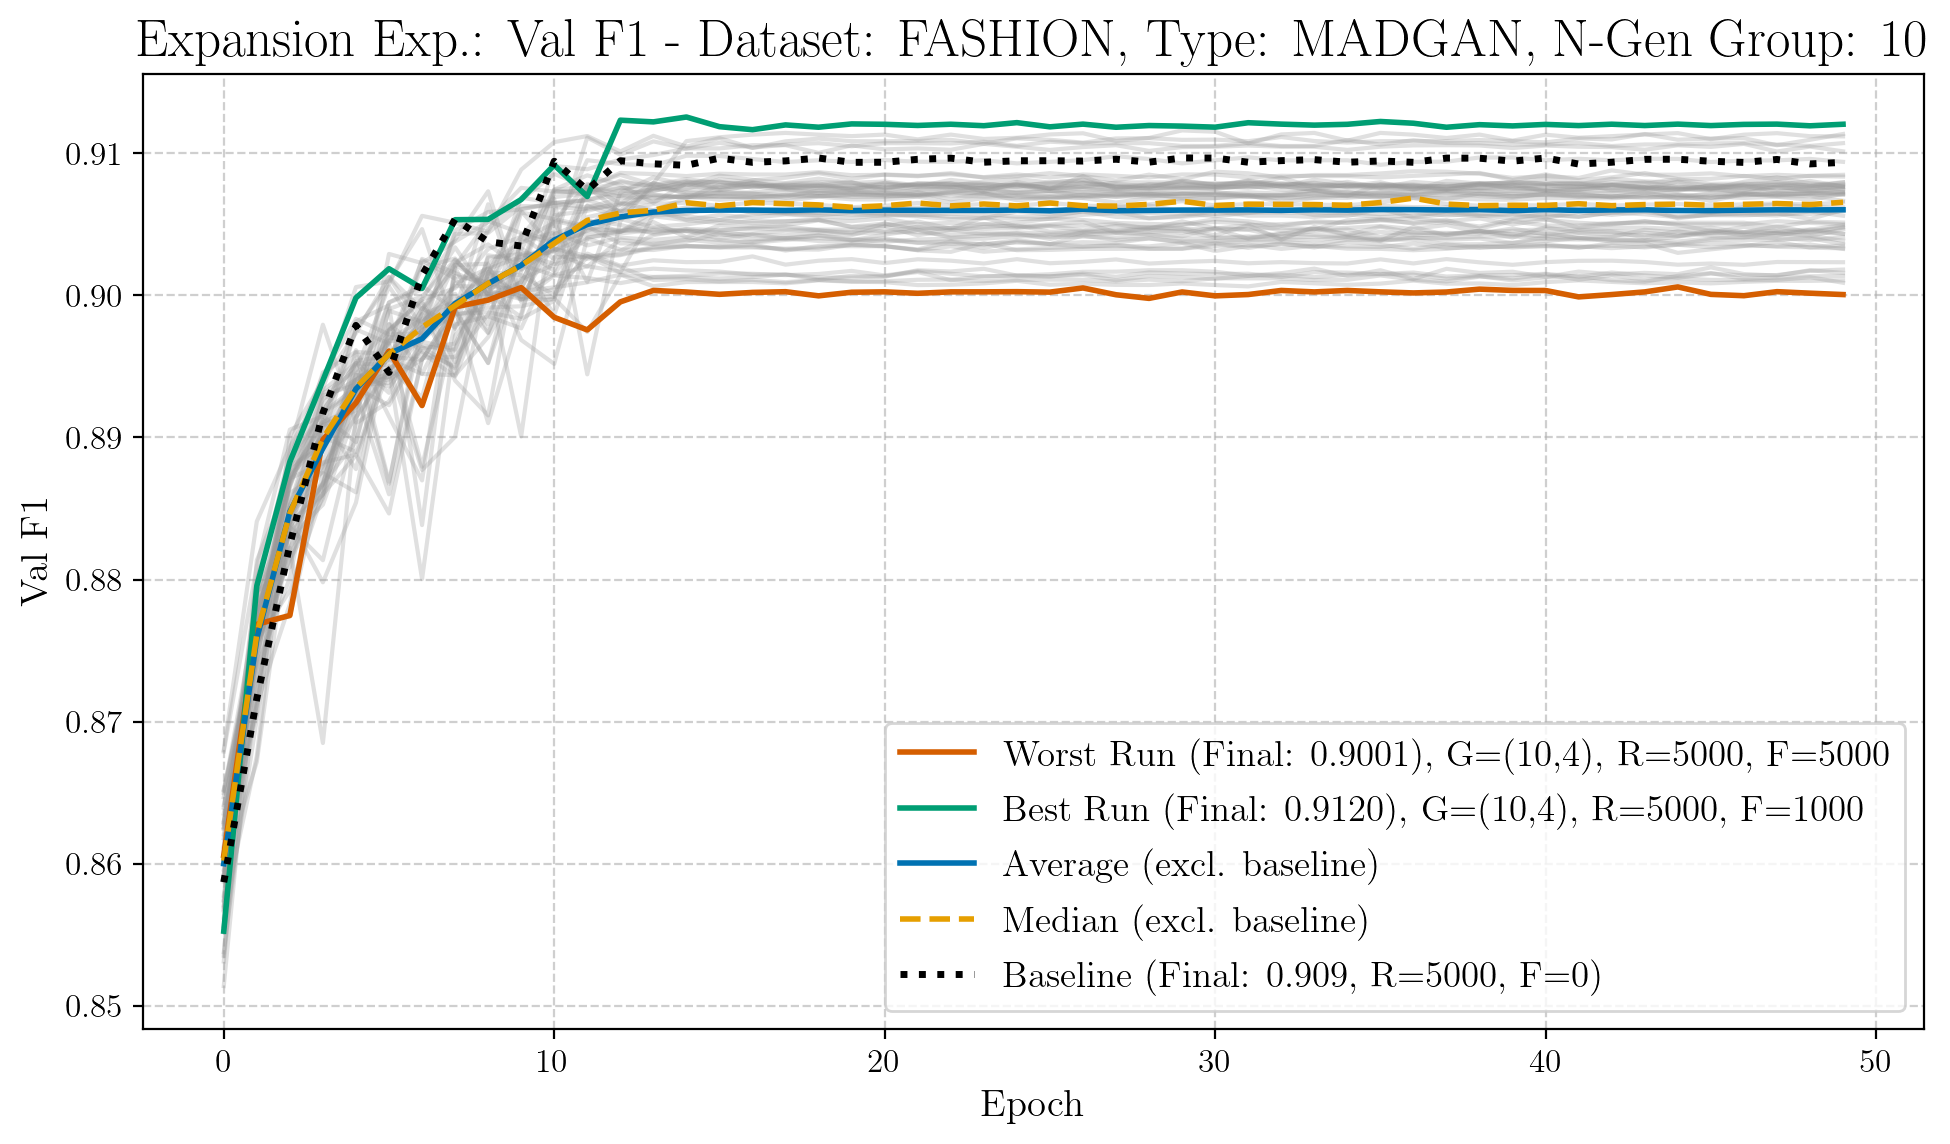
\includegraphics[width=\textwidth]{abb/strat_classifier_performance/FASHION_STRATIFIED_CLASSIFIERS_MADGAN_NEW/expansion_experiments/val_f1_score_MADGAN_FASHION_n_gen_10_all.png}
		\caption{F1 Score on FASHION over 50 epochs. Augmentation tech.: MADGAN (K=10)}
        \label{fig:res_expansion_fashion_cgan_vs_madgan__madgan}
	\end{subfigure}
	\begin{subfigure}{.85\textwidth}
		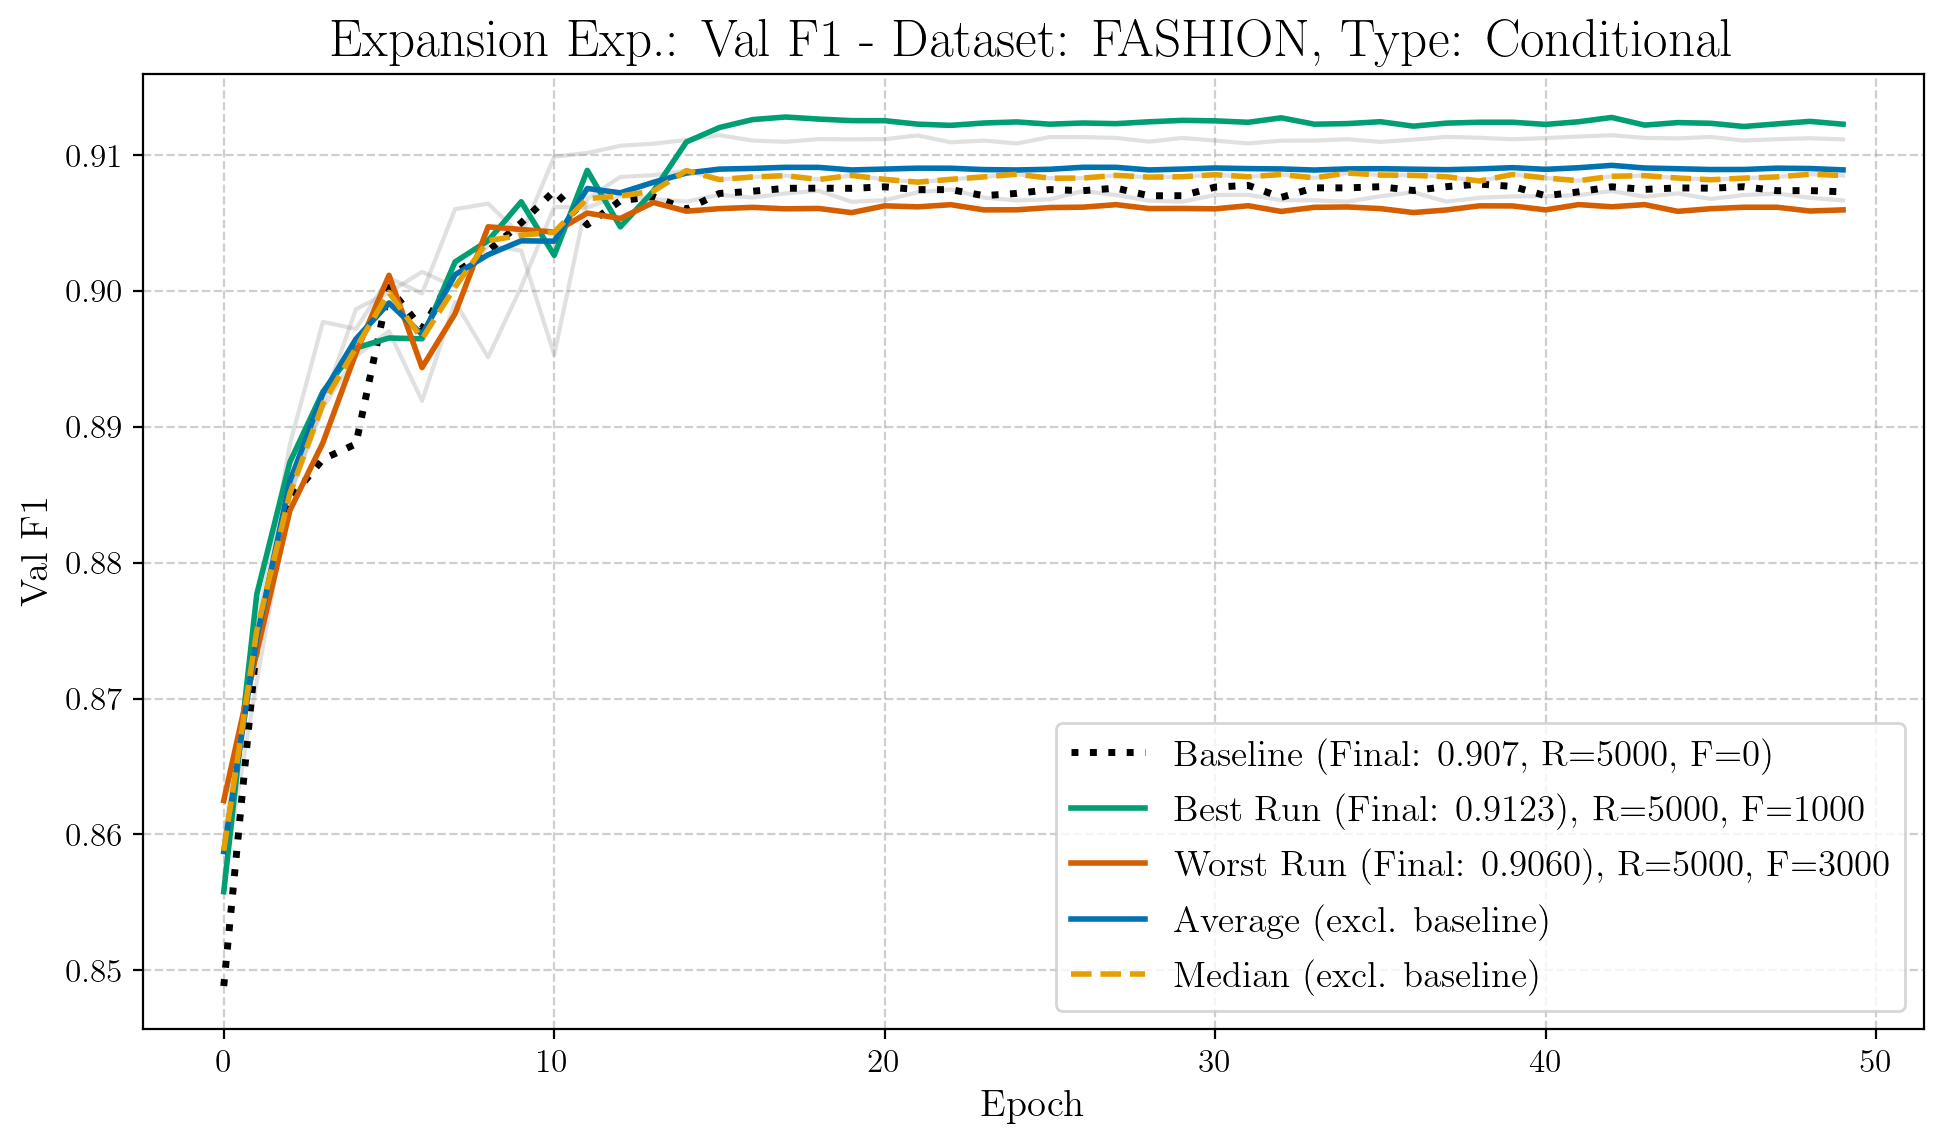
\includegraphics[width=\textwidth]{abb/strat_classifier_performance/FASHION_STRATIFIED_CLASSIFIERS_COND_GAN/expansion_experiments/val_f1_score_['COND']_FASHION_all.png}
		\caption{F1 Score on FASHION over 50 epochs. Augmentation Technique: cGAN}
        \label{fig:res_expansion_fashion_cgan_vs_madgan__cgan}
	\end{subfigure}
%%%%%%%%%%%%%%
\end{figure}

\begin{table}[H]
	\vspace{-1.5em}
	\centering
	\begin{tabular}{|c|c|c|c|}
		\hline
		Run Type & Experiment & Val F1 \\ \hline
		best & \(G_{10, 4}\), R:5000, F:1000 & $0.9120$\\ \hline
		worst & \(G_{10, 4}\), R:5000, F:5000 & $0.9001$\\ \hline
		median & G (K=10) & $0.9066$\\ \hline
		average & (K=10) & $0.9060$
		\\ \hline
	\end{tabular}
    \caption{Final F1 Scores after 50 epochs. Augmentation tech.: MADGAN (K=10)}
        \label{tab:res_expansion_fashion_cgan_vs_madgan__madgan}
\end{table}
\begin{table}[H]
	\centering
	\vspace{-1.5em}
	\begin{tabular}{|c|c|c|c|c|}
		\hline
		Run Type & Experiment & Val F1 \\ \hline
		best & Conditional (R:5000, F:1000) & $0.9123$\\ \hline
		worst & Conditional (R:5000, F:3000) & $0.9060$\\ \hline
		median & Conditional & $0.9085$\\ \hline
		average & Conditional & $0.9089$
		\\ \hline
	\end{tabular}
    \caption{Final F1 Scores after 50 epochs. Augmentation technique: cGAN}
        \label{tab:res_expansion_fashion_cgan_vs_madgan__cgan}
\end{table}

Both GDA approaches demonstrate effectiveness in the expansion scenario on Fashion-MNIST, achieving high F1 scores that suggest an improvement over a baseline trained on real data alone. The peak performances are very competitive: cGAN achieved a best F1 score of $0.9123$ (when adding ,000 synthetic samples), marginally edging out MADGAN K=10's best F1 score of $0.9120$ (also achieved when adding 1000 synthetic samples from its best generator, \(G_{10,4}\)). These top scores are notably close to the peak performance observed with TDA in previous comparisons.

However, cGAN exhibits slightly better overall consistency and robustness as more synthetic data is added. The average F1 score for cGAN across all expansion levels is $0.9089$, and its median is $0.9085$. These are slightly higher than MADGAN K=10's average ($0.9060$) and median ($0.9066$). More critically, cGAN's worst-case performance (F1 $0.9060$, when adding 3000 synthetic samples) is substantially better than MADGAN K=10's worst-case (F1 $0.9001$, occurring for generator \(G_{10,4}\) when adding 5000 synthetic samples). This indicates that cGAN's performance degrades less and remains more stable even with larger amounts of synthetic data compared to MADGAN K=10. Consequently, cGAN shows a tighter performance spread (range ~$0.0063$) than MADGAN K=10 (range ~$0.0119$).

In conclusion, for expanding the Fashion-MNIST dataset, both cGAN and MADGAN (K=10) GDA can provide performance benefits, achieving F1 scores competitive with traditional augmentation methods at their peak. However, cGAN demonstrates a slight advantage in overall performance, offering higher average and median scores, and particularly showing greater stability and less degradation when larger volumes of synthetic data are incorporated.

\newpage
\subsubsection[Question 4]{MADGAN GDA vs. cMADGAN GDA Performance}      \label{exp_results_ans_q4}
Ultimately, the final direct comparison sets MADGAN and the conditional adaptation cMADGAN side-by-side. As established before, the best selection of MADGAN experiments (K=10 for Replacement-, K=7 for Expansion scenario on MNIST and K=7 for Replacement-, K=10 for Expansion scenario on Fashion-MNIST) is directly compared against the best performing setting of cMADGAN. Orienting on the afore comparison against MADGAN vs. DCGAN/cGAN (\ref{exp_results_ans_q3}), other cMADGAN experiments are mentioned were fit.

TODO: preamble the results of the following experiments

\newpage

\noindent\textbf{Replacement Experiment, Dataset: MNIST}
\begin{figure}[H]
	\centering
	\begin{subfigure}{.85\textwidth}
		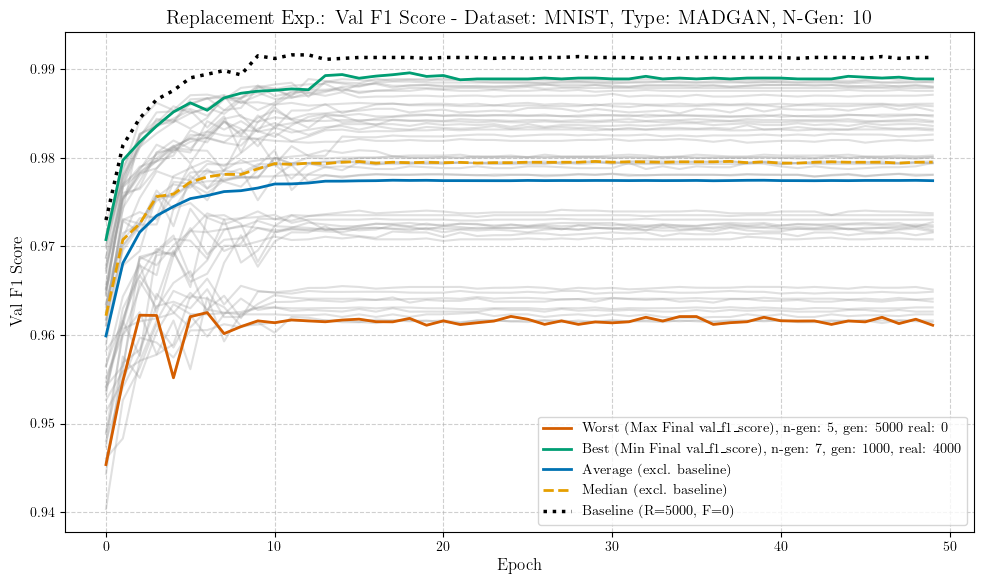
\includegraphics[width=\textwidth]{abb/strat_classifier_performance/MNIST_STRATIFIED_CLASSIFIERS_MADGAN_NEW/replacement_experiments/val_f1_score_MADGAN_MNIST_n_gen_10_all.png}
		\caption{F1 Score on MNIST over 50 epochs. Augmentation technique: MADGAN (K=10)}
        \label{fig:res_replacement_mnist_cmadgan_vs_madgan__madgan}
	\end{subfigure}
	\begin{subfigure}{.85\textwidth}
		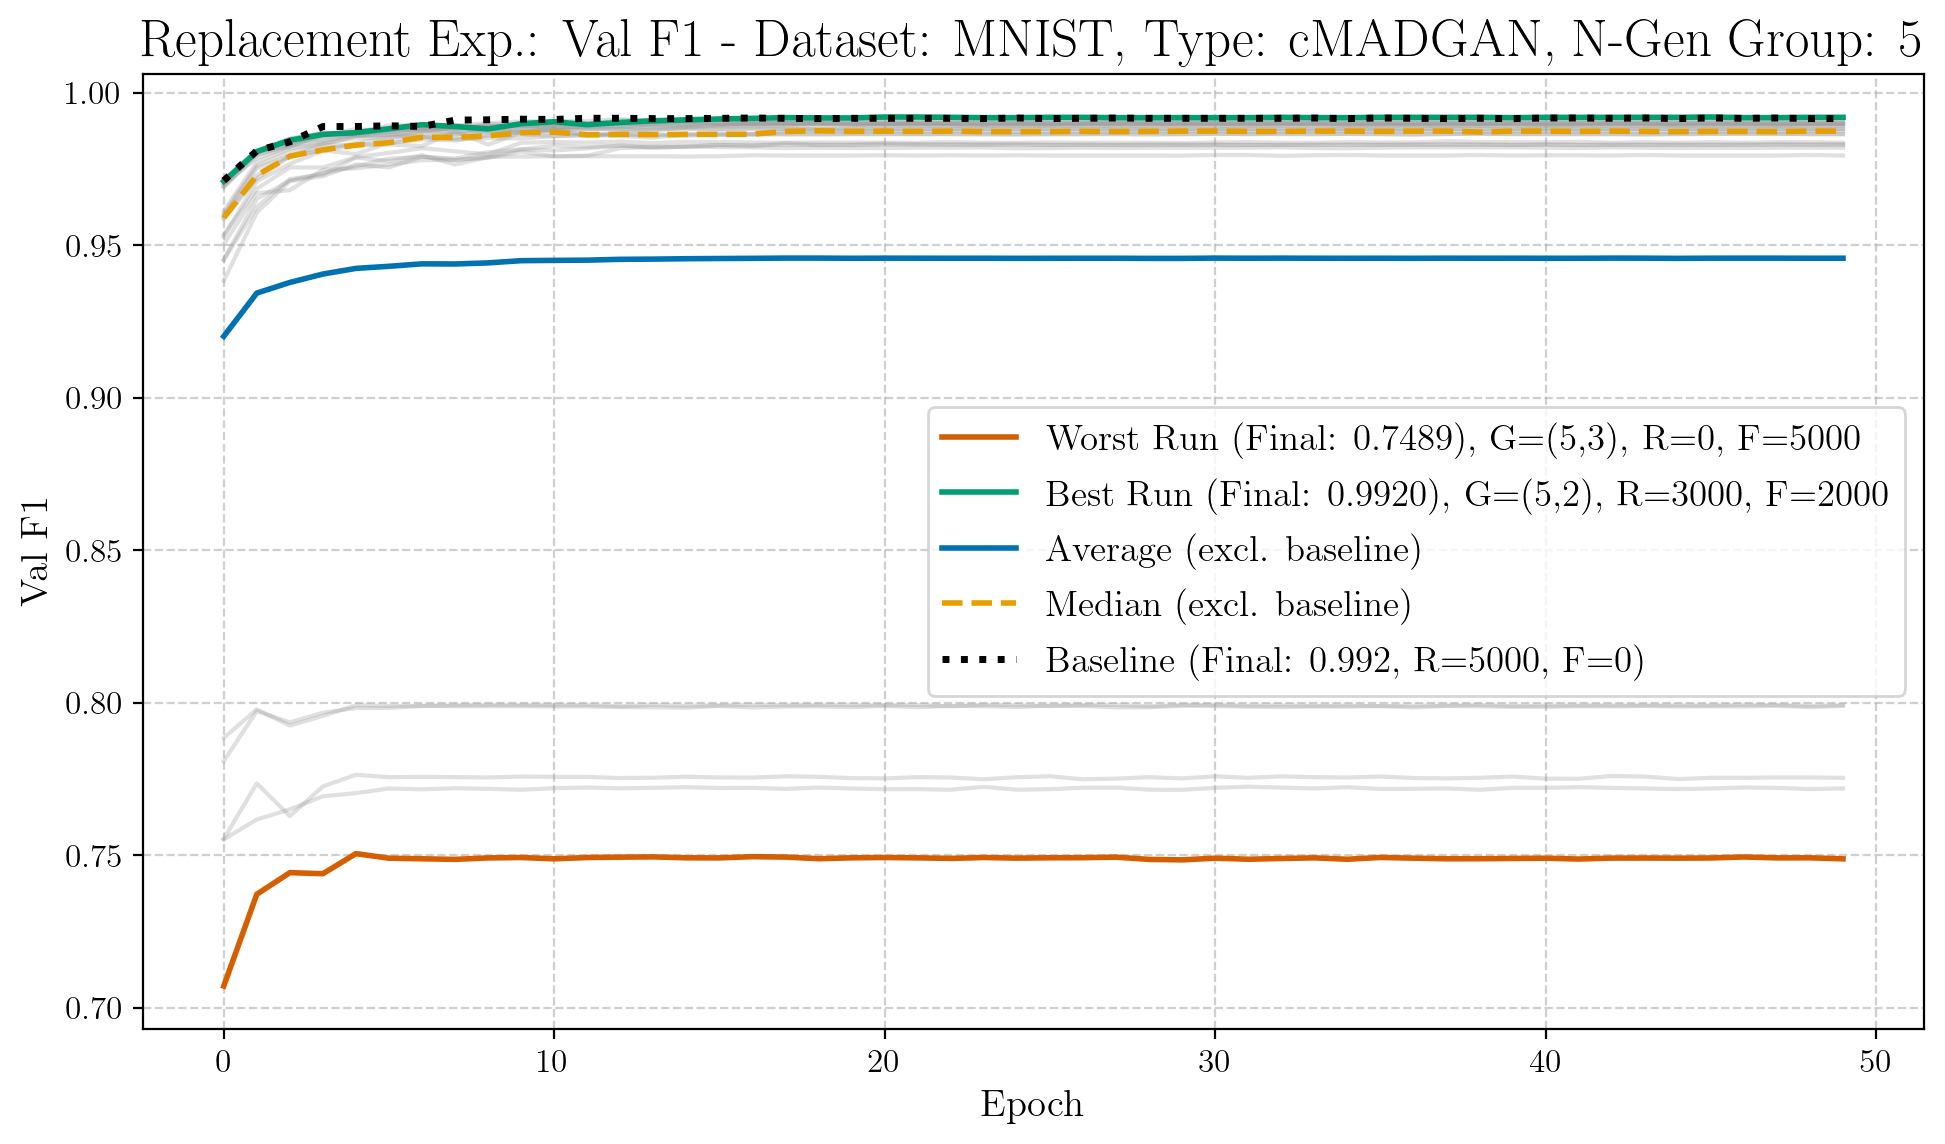
\includegraphics[width=\textwidth]{abb/strat_classifier_performance/MNIST_STRATIFIED_CLASSIFIERS_cMADGAN_NEW/replacement_experiments/val_f1_score_cMADGAN_MNIST_n_gen_5_all.png}
		\caption{F1 Score on MNIST over 50 epochs. Augmentation technique: cMADGAN (K=5)}
        \label{fig:res_replacement_mnist_cmadgan_vs_madgan__cmadgan}
	\end{subfigure}
%%%%%%%%%%%%%%
\end{figure}

\begin{table}[H]
	\vspace{-1.5em}
	\centering
	\begin{tabular}{|c|c|c|c|}
		\hline
		Run Type & Experiment & Val F1 \\ \hline
		best & \(G_{10, 7}\), R:4000, F:1000 & $0.9889$\\ \hline
		worst & \(G_{10, 5}\), R:0, F:5000 & $0.9611$\\ \hline
		median & G (K=10) & $0.9795$\\ \hline
		average & G (K=10) & $0.9774$
		\\ \hline
	\end{tabular}
    \caption{Final F1 Scores after 50 epochs. Augmentation technique: MADGAN (K=10)}
        \label{tab:res_replacement_mnist_cmadgan_vs_madgan__madgan}
\end{table}
\begin{table}[H]
	\centering
	\vspace{-1.5em}
	\begin{tabular}{|c|c|c|c|c|}
		\hline
		Run Type & Experiment & Val F1 \\ \hline
		best & \(G_{5, 2}\), R:3000, F:2000 & $0.9920$\\ \hline
		worst & \(G_{5, 3}\), R:0, F:5000 & $0.7489$\\ \hline
		median & G (K=5) & $0.9874$\\ \hline
		average & G (K=5) & $0.9458$
		\\ \hline
	\end{tabular}
    \caption{Final F1 Scores after 50 epochs. Augmentation technique: cMADGAN (K=5)}
        \label{tab:res_replacement_mnist_cmadgan_vs_madgan__cmadgan}
\end{table}
The comparison reveals a fascinating trade-off between peak performance potential and consistency. The cMADGAN (K=5) model achieved the highest individual F1 score in this set of experiments, reaching $0.9920$ (with generator \(G_{5,2}\) when replacing 2000 real samples with 2000 synthetic ones per class from the R:5000/F:0 baseline). This peak performance is notably high, surpassing the best score from MADGAN K=10 ($0.9889$) and even rivaling the top scores seen with Traditional Data Augmentation (TDA) in previous comparisons. This suggests that individual generators within the cMADGAN K=5 framework can produce highly effective synthetic data for replacement.

However, cMADGAN K=5 exhibits extreme variability. Its worst-performing run (generator \(G_{5,3}\) when using only synthetic data, R:0, F:5000) resulted in a drastically low F1 score of $0.7489$. This catastrophic drop for at least one of its generators signifies a lack of reliability. In contrast, MADGAN K=10, while not reaching the same peak as cMADGAN K=5, demonstrated much greater consistency. Its worst-case F1 score was $0.9611$, indicating that even its poorest performing generator at full replacement maintained a high level of performance.

This difference in variability heavily influences the average and median scores. MADGAN K=10 achieved a substantially better average F1 score ($0.9774$) compared to cMADGAN K=5 ($0.9458$), as the latter's average was significantly pulled down by its low outlier(s). Conversely, cMADGAN K=5 reported a higher median F1 score ($0.9874$) than MADGAN K=10 ($0.9795$), suggesting that the "typical" performance of a cMADGAN K=5 generator (excluding the worst cases) is very strong and even surpasses the typical MADGAN K=10 generator. The overall performance spread for cMADGAN K=5 (range ~$0.2431$) is vastly larger than that of MADGAN K=10 (range ~$0.0278$).

To conclude, for the replacement task on MNIST, cMADGAN (K=5) offers the potential for superior peak GDA performance from its best generators, achieving results competitive with the best augmentation methods. However, it suffers from significant inconsistency, with some generators producing very poor quality synthetic data leading to a low average performance. MADGAN (K=10) provides more reliable and stable GDA performance, with a better average F1 score and a much more dependable worst-case outcome, though its peak performance is slightly lower than the best of cMADGAN (K=5).


\newpage
\noindent\textbf{Expansion Experiment, Dataset: MNIST}
\begin{figure}[H]
	\centering
	\begin{subfigure}{.85\textwidth}
		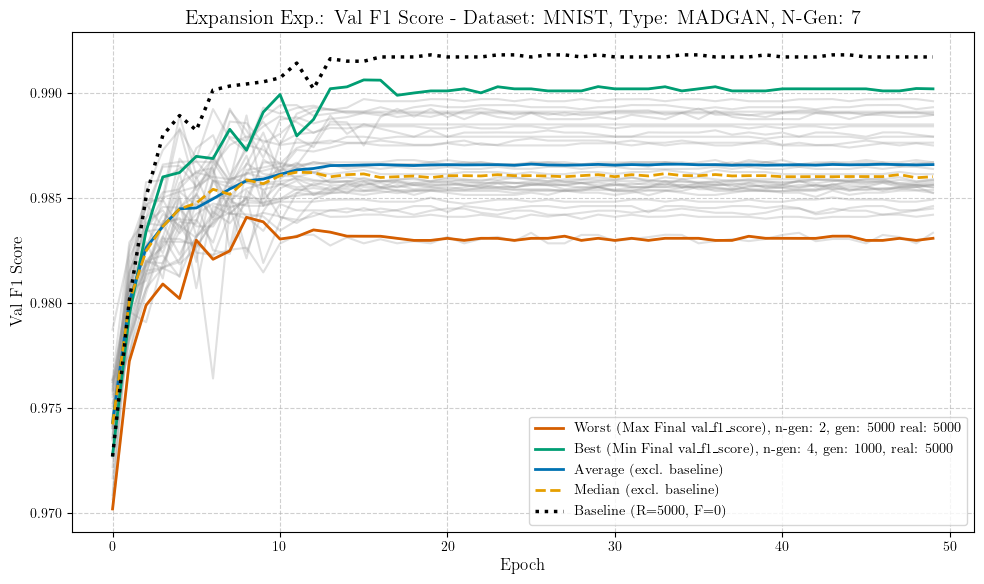
\includegraphics[width=\textwidth]{abb/strat_classifier_performance/MNIST_STRATIFIED_CLASSIFIERS_MADGAN_NEW/expansion_experiments/val_f1_score_MADGAN_MNIST_n_gen_7_all.png}
		\caption{F1 Score on MNIST over 50 epochs. Augmentation tech.: MADGAN (K=7)}
        \label{fig:res_expansion_mnist_cmadgan_vs_madgan__madgan}
	\end{subfigure}
	\begin{subfigure}{.85\textwidth}
		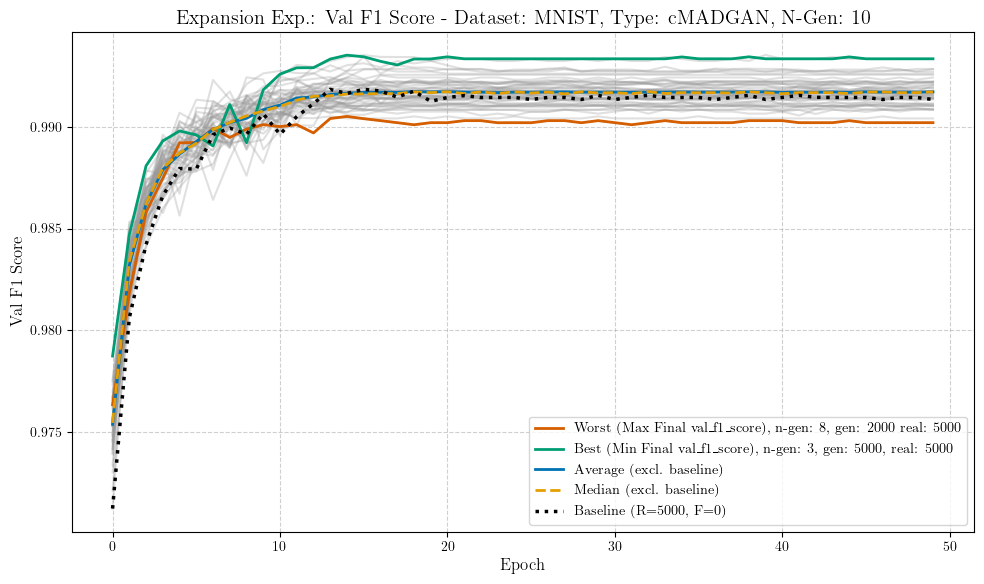
\includegraphics[width=\textwidth]{abb/strat_classifier_performance/MNIST_STRATIFIED_CLASSIFIERS_cMADGAN_NEW/expansion_experiments/val_f1_score_cMADGAN_MNIST_n_gen_10_all.png}
		\caption{F1 Score on MNIST over 50 epochs. Augmentation tech.: cMADGAN (K=10)}
        \label{fig:res_expansion_mnist_cmadgan_vs_madgan__cmadgan}
	\end{subfigure}
%%%%%%%%%%%%%%
\end{figure}

\begin{table}[H]
	\vspace{-1.5em}
	\centering
	\begin{tabular}{|c|c|c|c|}
		\hline
		Run Type & Experiment & Val F1 \\ \hline
		best & \(G_{7, 4}\), R:5000, F:1000 & $0.9902$\\ \hline
		worst & \(G_{7, 2}\), R:5000, F:5000 & $0.9831$\\ \hline
		median & G (K=7) & $0.9860$\\ \hline
		average & G (K=7) & $0.9866$
		\\ \hline
	\end{tabular}
    \caption{Final F1 Scores after 50 epochs. Augmentation tech.: MADGAN (K=10)}
        \label{tab:res_expansion_mnist_cmadgan_vs_madgan__madgan}
\end{table}
\begin{table}[H]
	\centering
	\vspace{-1.5em}
	\begin{tabular}{|c|c|c|c|c|}
		\hline
		Run Type & Experiment & Val F1 \\ \hline
		best & \(G_{10, 3}\), R:5000, F:5000 & $0.9933$\\ \hline
		worst & \(G_{10, 8}\), R:5000, F:2000 & $0.9902$\\ \hline
		median & G (K=10) & $0.9917$\\ \hline
		average & G (K=10) & $0.9917$
		\\ \hline
	\end{tabular}
    \caption{Final F1 Scores after 50 epochs. Augmentation tech.: cMADGAN (K=10)}
        \label{tab:res_expansion_mnist_cmadgan_vs_madgan__cmadgan}
\end{table}

The results compellingly demonstrate the superiority of cMADGAN (K=10) over MADGAN (K=7) for data expansion on MNIST. Across all summary statistics, cMADGAN (K=10) achieves markedly better and more consistent F1 scores.

Specifically, the best F1 score attained by cMADGAN (K=10) is $0.9933$ (generator \(G_{10,3}\) when adding 5000 synthetic samples), which is not only significantly higher than MADGAN K=7's best of $0.9902$ but is also highly competitive with the peak performance observed using Traditional Data Augmentation (TDA, previously around $0.9938$). Remarkably, this peak for cMADGAN K=10 occurs at the maximum level of data expansion (F:5000), indicating a strong positive contribution from the synthetic data.

The robustness of cMADGAN K=10 is further highlighted by its worst-case performance. Its lowest F1 score across all its generators and expansion ratios is $0.9902$. Strikingly, this "worst" score for cMADGAN K=10 is identical to the "best" score achieved by MADGAN K=7. In contrast, MADGAN K=7's performance drops to $0.9831$ in its worst-case scenario.

Consequently, the average ($0.9917$) and median ($0.9917$) F1 scores for cMADGAN K=10 are substantially higher than those for MADGAN K=7 (average $0.9866$, median $0.9860$). Moreover, cMADGAN K=10 exhibits a much tighter performance cluster, with a very small spread between its best and worst scores (range ~$0.0031$), indicating high consistency across its generators and different levels of augmentation. This contrasts with MADGAN K=7's larger spread (range ~$0.0071$).

In conclusion, for the MNIST expansion task, cMADGAN (K=10) GDA proves to be a significantly more effective and reliable augmentation technique than MADGAN (K=7) GDA. It not only achieves higher peak performance that rivals traditional methods but also maintains excellent scores with minimal variability even when large volumes of synthetic data are introduced, showcasing its strong potential for enhancing classifier training.


\newpage
\noindent\textbf{Replacement Experiment, Dataset: Fashion-MNIST}
\begin{figure}[H]
	\centering
	\begin{subfigure}{.85\textwidth}
		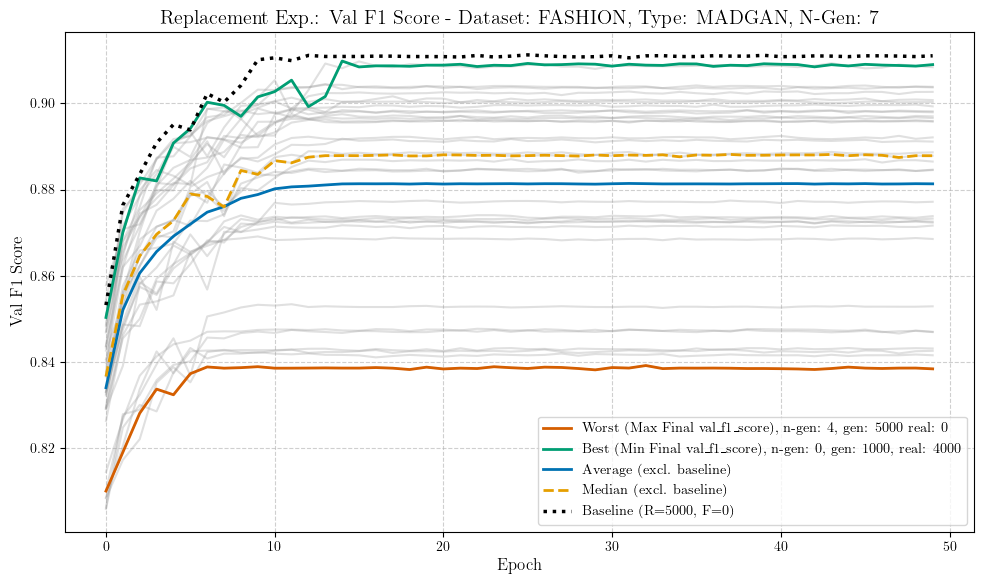
\includegraphics[width=\textwidth]{abb/strat_classifier_performance/FASHION_STRATIFIED_CLASSIFIERS_MADGAN_NEW/replacement_experiments/val_f1_score_MADGAN_FASHION_n_gen_7_all.png}
		\caption{F1 Score on FASHION over 50 epochs. Augmentation tech.: MADGAN (K=7)}
        \label{fig:res_replacement_fashion_cmadgan_vs_madgan__madgan}
	\end{subfigure}
	\begin{subfigure}{.85\textwidth}
		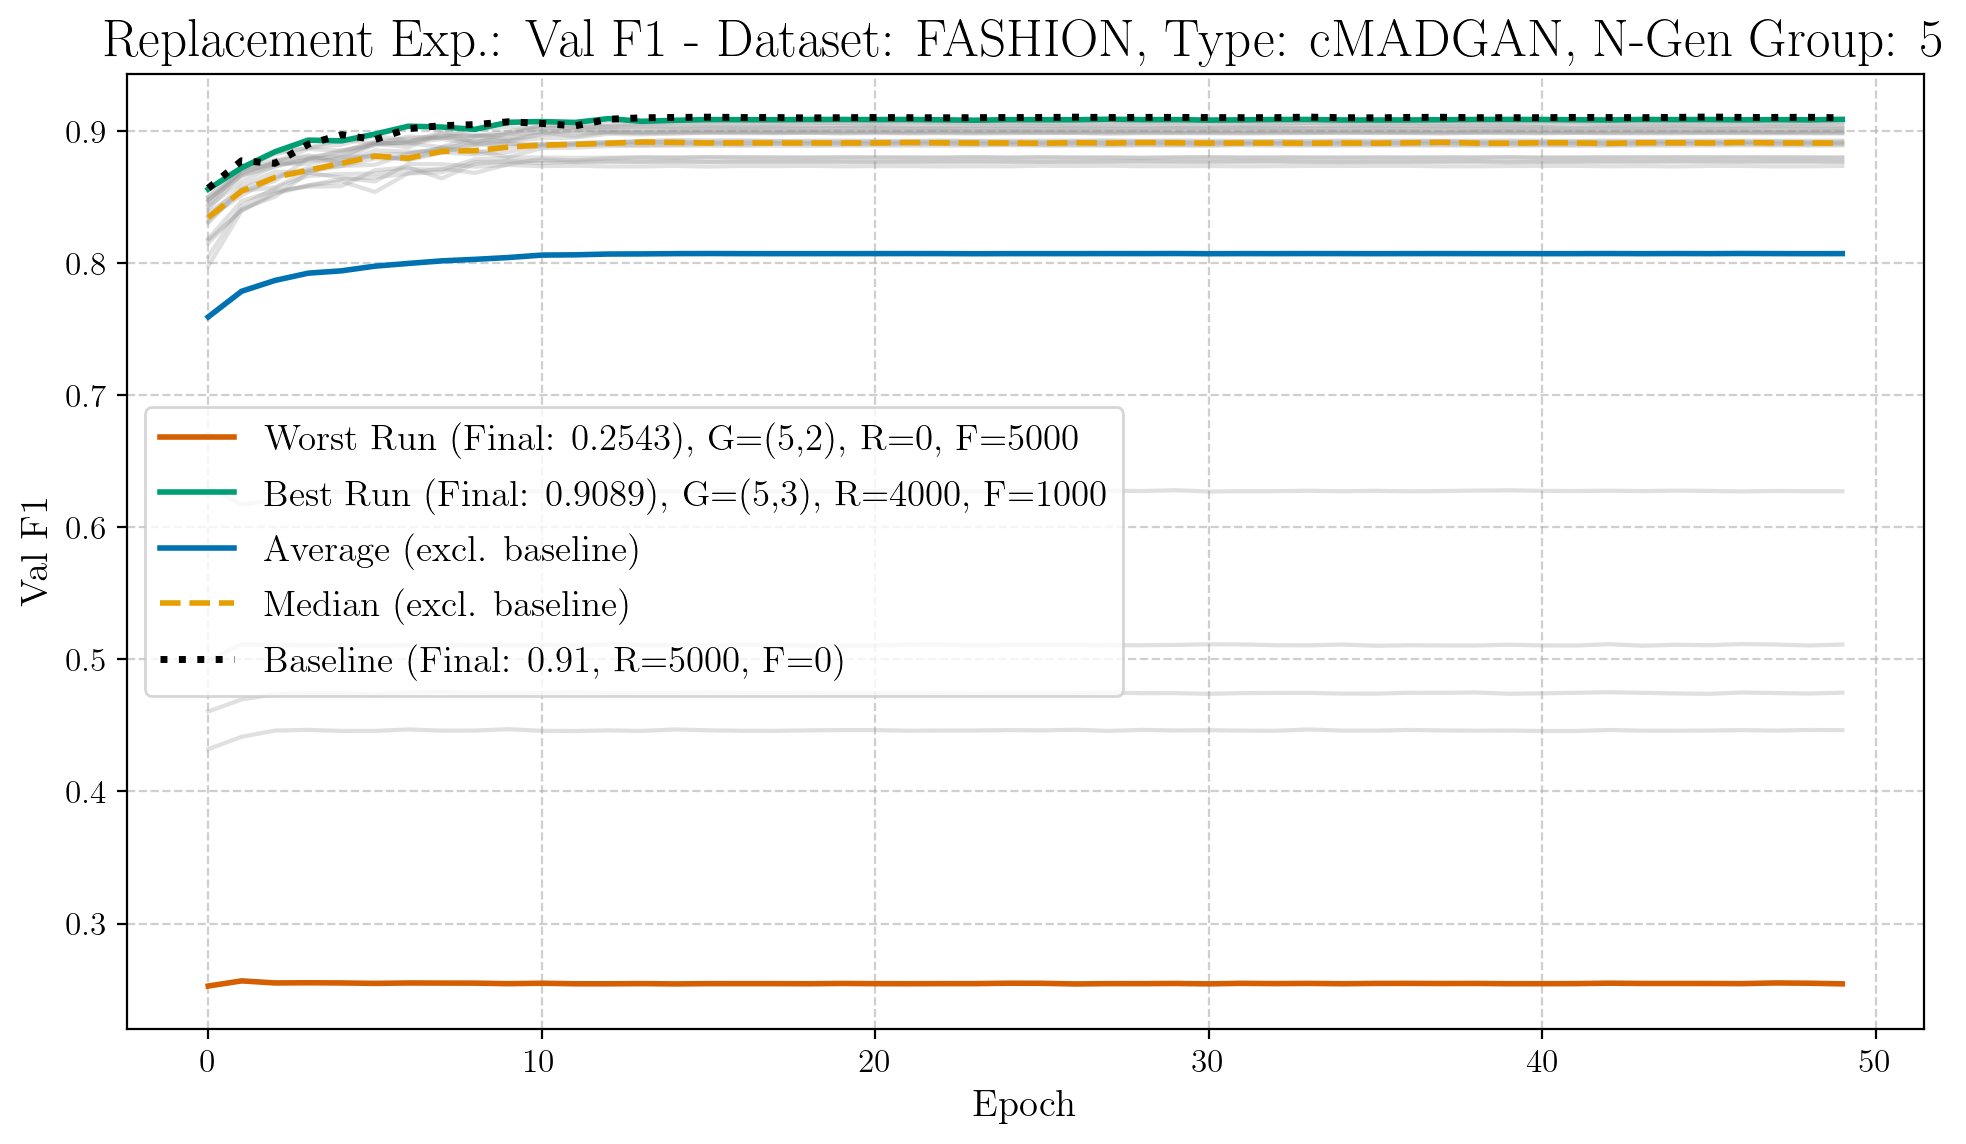
\includegraphics[width=\textwidth]{abb/strat_classifier_performance/FASHION_STRATIFIED_CLASSIFIERS_cMADGAN_NEW/replacement_experiments/val_f1_score_cMADGAN_FASHION_n_gen_5_all.png}
		\caption{F1 Score on FASHION over 50 epochs. Augmentation tech.: cMADGAN (K=5)}
        \label{fig:res_replacement_fashion_cmadgan_vs_madgan__cmadgan}
	\end{subfigure}
%%%%%%%%%%%%%%
\end{figure}

\begin{table}[H]
	\vspace{-1.5em}
	\centering
	\begin{tabular}{|c|c|c|c|}
		\hline
		Run Type & Experiment & Val F1 \\ \hline
		best & \(G_{7, 2}\), R:4000, F:1000 & $0.9079$\\ \hline
		worst & \(G_{7, 0}\), R:0, F:5000 & $0.3419$\\ \hline
		median & G = (K=7) & $0.8927$\\ \hline
		average & G = (K=7) & $0.7993$
		\\ \hline
	\end{tabular}
    \caption{Final F1 Scores after 50 epochs. Augmentation tech.: MADGAN (K=7)}
        \label{tab:res_replacement_fashion_cmadgan_vs_madgan__madgan}
\end{table}
\begin{table}[H]
	\centering
	\vspace{-1.5em}
	\begin{tabular}{|c|c|c|c|c|}
		\hline
		Run Type & Experiment & Val F1 \\ \hline
		best & \(G_{5, 3}\), R:4000, F:1000 & $0.9089$\\ \hline
		worst & \(G_{5, 2}\), R:0, F:5000 & $0.2543$\\ \hline
		median & G (K=5) & $0.8909$\\ \hline
		average & G (K=5) & $0.8072$
		\\ \hline
	\end{tabular}
    \caption{Final F1 Scores after 50 epochs. Augmentation tech.: cMADGAN (K=5)}
        \label{tab:res_replacement_fashion_cmadgan_vs_madgan__cmadgan}
\end{table}

Both multi-generator approaches demonstrate the capability to achieve high peak F1 scores when a limited amount of real data is replaced. cMADGAN (K=5) achieved a slightly higher best F1 score of $0.9089$ (generator \(G_{5,3}\) with R:4000, F:.000), marginally surpassing MADGAN K=7's best of $0.9079$ (generator \(G_{7,2}\) with R:4000, F:1000). Notably, these peak performances from both models are competitive with, and even slightly exceed, the best scores previously observed with Traditional Data Augmentation (TDA) on this dataset.

However, this high peak potential is starkly contrasted by extreme inconsistency and poor performance when relying heavily on synthetic data, particularly when all real data is substituted. cMADGAN (K=5) exhibited the lowest worst-case F1 score, dropping to a catastrophic $0.2543$ (generator \(G_{5,2}\) with R:0, F:5000). While MADGAN K=7's worst-case ($0.3419$ from generator \(G_{7,0}\) with R:0, F:5000) was also severely degraded, it remained slightly above cMADGAN K=5's absolute floor.

These extreme low scores significantly impact the overall assessment. Despite its slightly lower absolute worst score, cMADGAN (K=5) managed a slightly higher average F1 score ($0.8072$) compared to MADGAN K=7 ($0.7993$). This suggests that, aside from its most extreme outliers, the bulk of cMADGAN K=5's generator/ratio combinations might perform marginally better than those of MADGAN K=7. Conversely, MADGAN K=7 shows a slightly better median F1 score ($0.8927$) than cMADGAN K=5 ($0.8909$), indicating its "typical" performance, discounting the severe negative outliers from both, might be marginally more consistent. Both models display very large performance spreads, with cMADGAN K=5 having a marginally wider range due to its lower floor.

In conclusion, for the Fashion-MNIST replacement task, both MADGAN (K=7) and cMADGAN (K=5) can produce synthetic data from their best generators that lead to excellent, TDA-competitive classifier performance with limited replacement. However, both frameworks suffer from extreme variability and contain individual generators that produce very poor-quality data for this task, leading to unusable classifiers when real data is fully replaced. While cMADGAN K=5 achieved a marginally higher peak and average, its worst-case was more severe, making both models unreliable for extensive data replacement compared to more stable traditional methods, despite their promising best-case results.


\newpage
\noindent\textbf{Expansion Experiment, Dataset: Fashion-MNIST}
\begin{figure}[H]
	\centering
	\begin{subfigure}{.85\textwidth}
		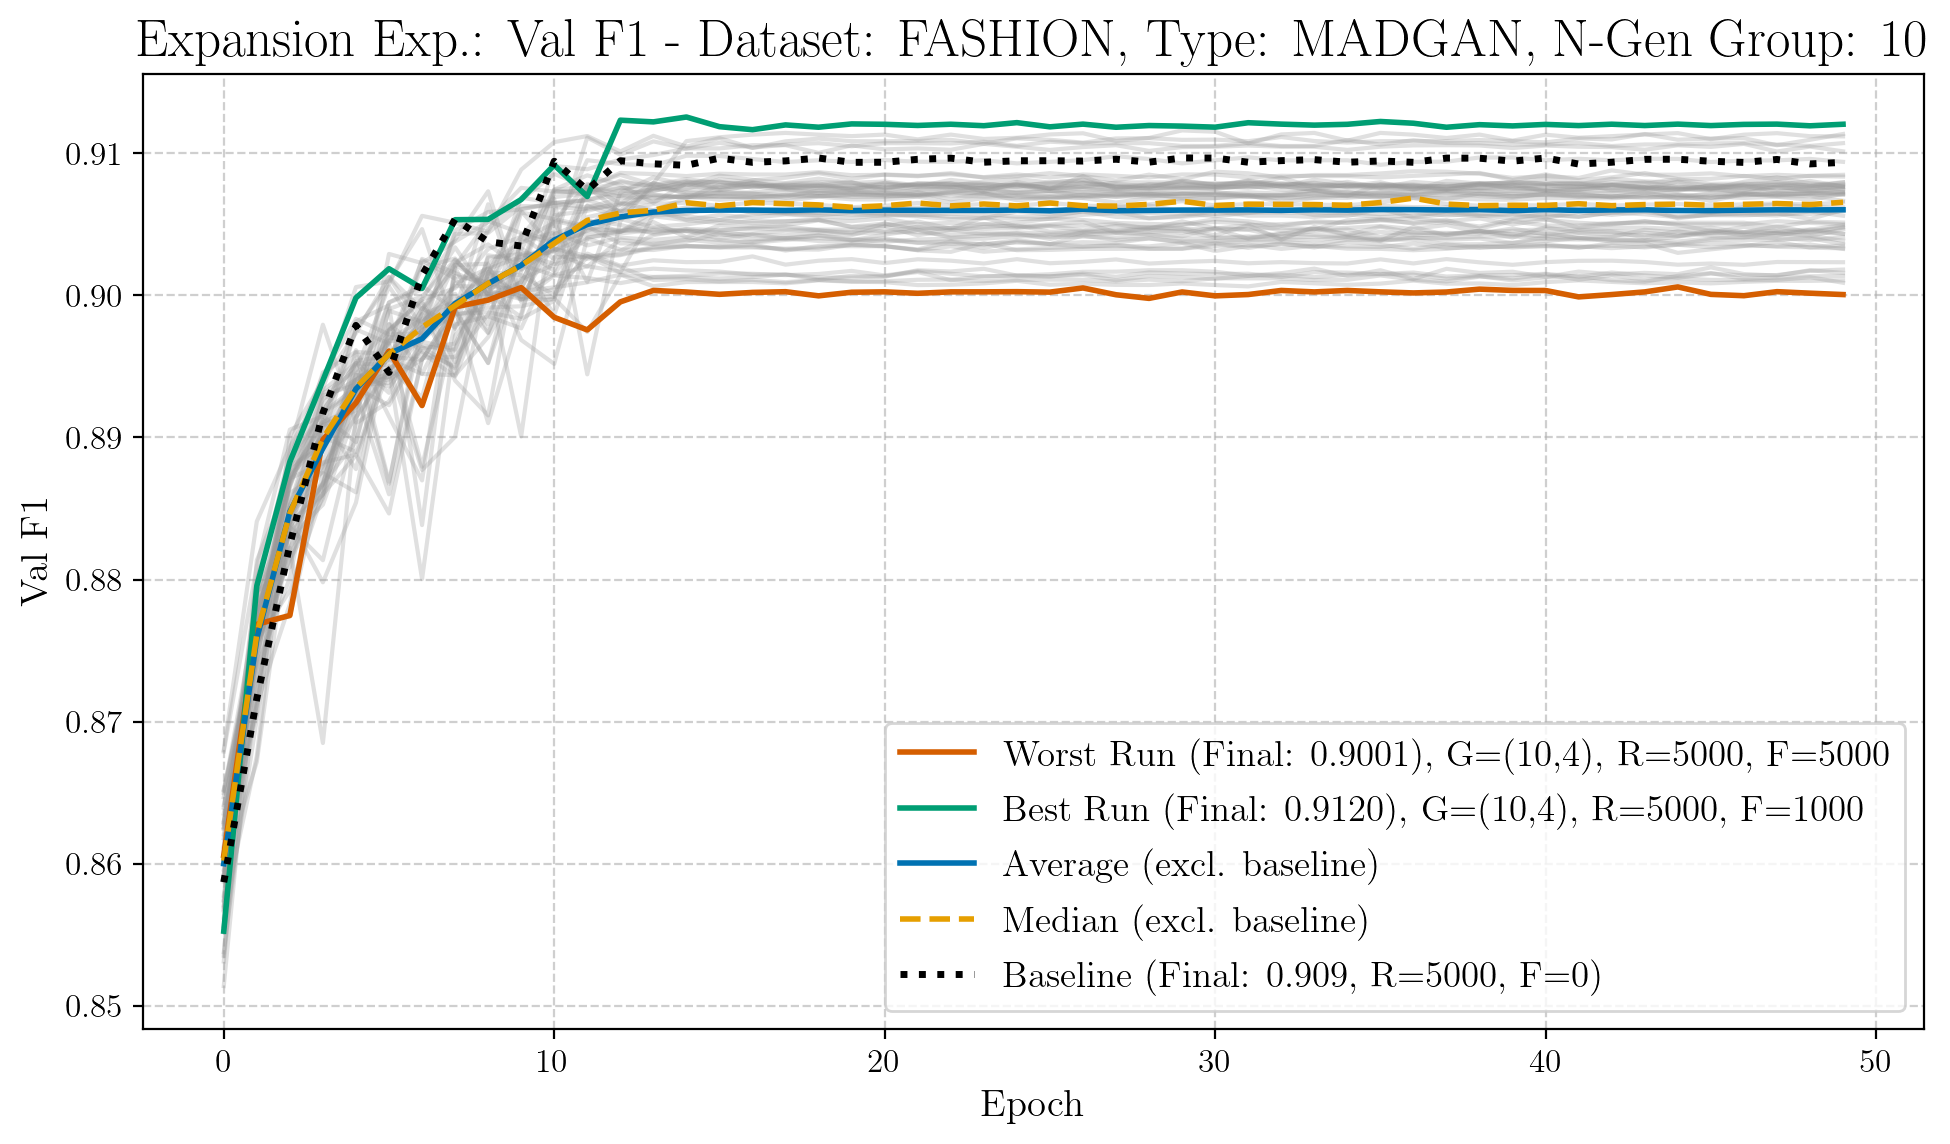
\includegraphics[width=\textwidth]{abb/strat_classifier_performance/FASHION_STRATIFIED_CLASSIFIERS_MADGAN_NEW/expansion_experiments/val_f1_score_MADGAN_FASHION_n_gen_10_all.png}
		\caption{F1 Score on FASHION over 50 epochs. Augmentation tech.: MADGAN (K=10)}
        \label{fig:res_expansion_fashion_cmadgan_vs_madgan__madgan}
	\end{subfigure}
	\begin{subfigure}{.85\textwidth}
		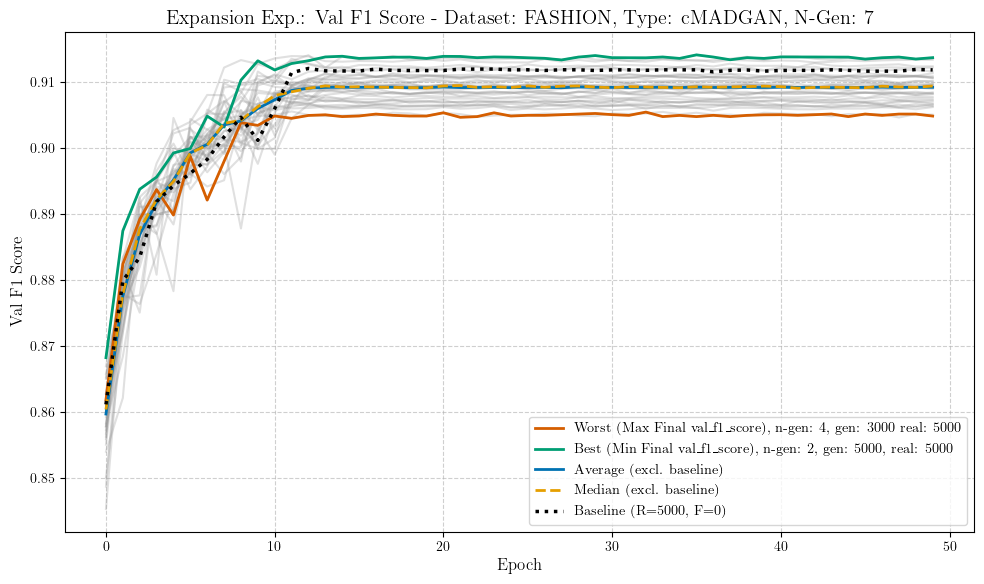
\includegraphics[width=\textwidth]{abb/strat_classifier_performance/FASHION_STRATIFIED_CLASSIFIERS_cMADGAN_NEW/expansion_experiments/val_f1_score_cMADGAN_FASHION_n_gen_7_all.png}
		\caption{F1 Score on FASHION over 50 epochs. Augmentation tech.: cMADGAN (K=7)}
        \label{fig:res_expansion_fashion_cmadgan_vs_madgan__cmadgan}
	\end{subfigure}
%%%%%%%%%%%%%%
\end{figure}

\begin{table}[H]
	\vspace{-1.5em}
	\centering
	\begin{tabular}{|c|c|c|c|}
		\hline
		Run Type & Experiment & Val F1 \\ \hline
		best & \(G_{10, 4}\), R:5000, F:1000 & $0.9120$\\ \hline
		worst & \(G_{10, 4}\), R:5000, F:5000 & $0.9001$\\ \hline
		median & G (K=10) & $0.9066$\\ \hline
		average & (K=10) & $0.9060$
		\\ \hline
	\end{tabular}
    \caption{Final F1 Scores after 50 epochs. Augmentation tech.: MADGAN (K=10)}
        \label{tab:res_expansion_fashion_cmadgan_vs_madgan__madgan}
\end{table}
\begin{table}[H]
	\centering
	\vspace{-1.5em}
	\begin{tabular}{|c|c|c|c|c|}
		\hline
		Run Type & Experiment & Val F1 \\ \hline
		best & \(G_{7, 2}\), R:5000, F:5000 & $0.9138$\\ \hline
		worst & \(G_{7, 4}\), R:5000, F:3000 & $0.9049$\\ \hline
		median & G (K=7) & $0.9095$\\ \hline
		average & G (K=7) & $0.9093$
		\\ \hline
	\end{tabular}
    \caption{Final F1 Scores after 50 epochs. Augmentation tech.: cMADGAN (K=7)}
        \label{tab:res_expansion_fashion_cmadgan_vs_madgan__cmadgan}
\end{table}

The results indicate a clear advantage for cMADGAN (K=7) over MADGAN (K=10) in this expansion scenario on Fashion-MNIST, with cMADGAN (K=7) demonstrating superior performance across all aggregated metrics.

cMADGAN (K=7) achieved a remarkable peak F1 score of $0.9138$ (with generator \(G_{7,2}\) when adding the maximum of 5000 synthetic samples per class). This is the highest F1 score recorded among all GDA methods on Fashion-MNIST in these expansion experiments and is highly competitive with the best scores from Traditional Data Augmentation (TDA, previously $0.9129$). The fact that this peak occurs at maximum data expansion is particularly noteworthy. Furthermore, cMADGAN K=7's worst-case F1 score ($0.9049$) is impressively high, indicating strong performance even from its least effective generator/ratio combination.

In comparison, MADGAN (K=10) achieved a best F1 score of $0.9120$ (generator \(G_{10,4}\) with R:5000, F:1000), slightly below cMADGAN K=7's peak. More significantly, MADGAN K=10's worst-case F1 score dropped to $0.9001$, which, while still good, is notably lower than cMADGAN K=7's worst case.

This superiority of cMADGAN K=7 is further reflected in its average ($0.9093$) and median ($0.9095$) F1 scores, both of which are higher than MADGAN K=10's average ($0.9060$) and median ($0.9066$). Additionally, cMADGAN (K=7) exhibited a tighter performance distribution, with a smaller spread between its best and worst scores (range ~$0.0089$) compared to MADGAN K=10 (range ~$0.0119$), signifying greater consistency.

In conclusion, for the Fashion-MNIST expansion task, cMADGAN (K=7) emerges as the more effective and reliable GDA technique compared to MADGAN (K=10). It not only achieves a higher peak F1 score that rivals TDA but also delivers better average performance and greater robustness, maintaining strong results even when substantially expanding the dataset with synthetic samples.

\subsubsection[Question 5]{Impact of MADGAN Generator Count}            \label{exp_results_ans_q5}



\newpage


\section{Outlook}\label{ausblick}

% develop a resiliant system for mad gan to generate data
% create a meta study, to compare the performance of different gan architectures

repair networks
\cite{Tanno2022repairingneuralnetworkfromcorrupt}


\newpage


\section{Conclusion}\label{conclusion}

Data generated by a GAN, may it be a cGAN or a MADGAN, may not fully capturethe distribution characteristics of its training data. Though, generated images do visually appear realistic, they may only partially reflect the statistical characteristics of the original data. This can lead to synthetic images that appear \textit{good} to a human inspector, but may contain amounts of noice that may interfere with a subsequent classifier.

%% Goood answer:
from an information theoratival standpoint, a generative model G trained on data X, distilling knowledge into a classifier C should not offer more information that what was already present in X.
%% https://www.reddit.com/r/MachineLearning/comments/s88s72/comment/htfud7b/?utm_source=share&utm_medium=web3x&utm_name=web3xcss&utm_term=1&utm_content=share_button
%% generally, the entire thread is an interesting critical POW against GANs for GDA in genral


Future research could focus on directly evaluating the impact of using MAD-GAN generated samples for augmenting various image classification datasets across different domains and comparing the resulting performance gains with those achieved by traditional and other generative augmentation techniques. Exploring methods to exert more control over the types of variations generated by MAD-GAN to specifically target weaknesses or improve the robustness of classifiers against particular types of noise or adversarial attacks would also be a valuable direction. Additionally, investigating the computational efficiency and scalability of training MAD-GAN for very large and complex datasets in the context of practical data augmentation pipelines would be crucial for its wider adoption. Finally, exploring the applicability of the MAD-GAN framework to generate diverse augmented data for other computer vision tasks beyond image classification, as well as for other data modalities such as natural language processing or audio processing, could further broaden its impact. The work by Ghosh et al. on Multi-Agent Diverse GANs represents a promising step towards leveraging the power of generative models for more effective and robust data augmentation in image classification and beyond.


% einfacher Zeilenabstand
\singlespacing
% Literaturliste soll im Inhaltsverzeichnis auftauchen
\newpage
\addcontentsline{toc}{section}{List of References}
% Literaturverzeichnis anzeigen
\renewcommand\refname{List of References}
% Add your citations here
\bibliography{main.bib}

%% Index soll Stichwortverzeichnis heissen
% \newpage
% % Stichwortverzeichnis soll im Inhaltsverzeichnis auftauchen
% \addcontentsline{toc}{section}{Stichwortverzeichnis}
% \renewcommand{\indexname}{Stichwortverzeichnis}
% % Stichwortverzeichnis endgültig anzeigen
% \printindex

\onehalfspacing
% evtl. Anhang
\newpage
\addcontentsline{toc}{section}{Appendix}
\fancyhead[L]{Appendix} %Kopfzeile links
\section*{Appendix}\label{appendix}

\setcounter{page}{1}

\subsection{Network Architectures}
The following section includes graphical representations of NN referenced throughout the thesis. %TODO: briefly describe the kindf of archs shown in this section...

\subsubsection{Classifiers}\label{appendix_classifiers}
The graphical representations of the network architectures are created with the tool \textit{visual keras}, by Paul Gavrikov (\cite{Gavrikov2020VisualKeras}).

\begin{figure}[htbp]
    \centering
    \vspace{-.5em}
    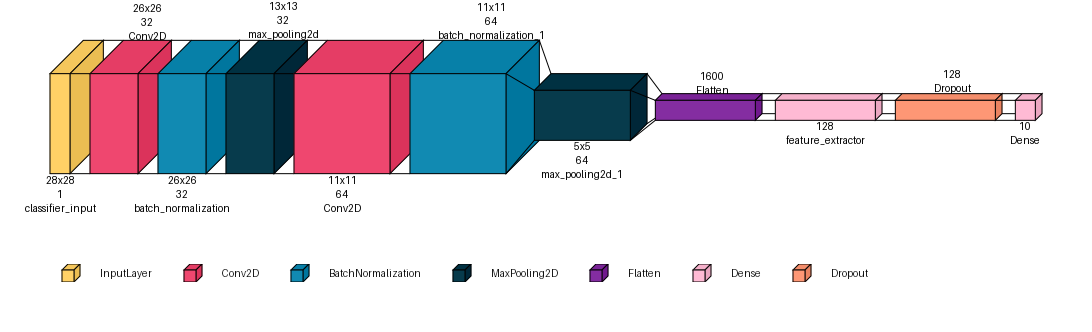
\includegraphics[width=.9\textwidth]{abb/netron_network_archs/classifying_Classifier_MNIST.png}
    \caption{Depiction of the CNN architecture used to classify unlabeled images from the MNIST GDA experiments and judge the effectiveness of said GDA. (Image created with \cite{Gavrikov2020VisualKeras})}
    \label{fig:figure_class_mnist}
\end{figure}

\begin{figure}[htbp]
    \centering
    \vspace{-2em}
    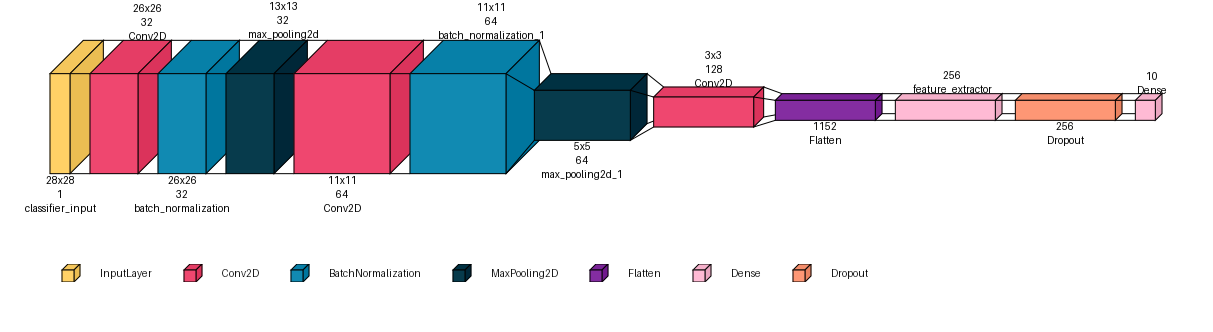
\includegraphics[width=.9\textwidth]{abb/netron_network_archs/classifying_Classifier_FashionMNIST.png}
    \caption{Depiction of the CNN architecture used to classify unlabeled images from the Fashion-MNIST GDA experiments and judge the effectiveness of said GDA. (Image created with \cite{Gavrikov2020VisualKeras})}
    \label{fig:figure_class_fashion}
\end{figure}

\begin{figure}[htbp]
    \centering
    \vspace{-2em}
    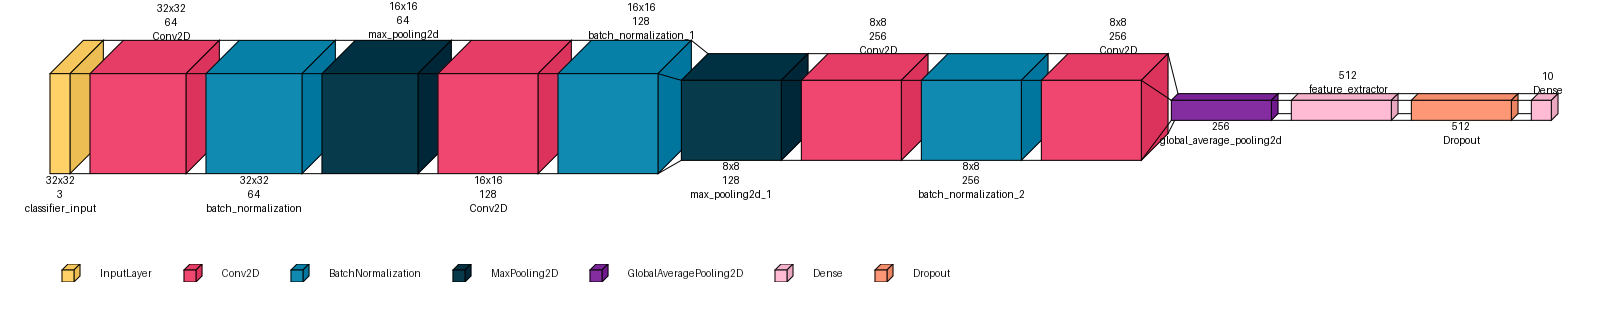
\includegraphics[width=.9\textwidth]{abb/netron_network_archs/classifying_Classifier_Cifar10.png}
    \caption{Depiction of the CNN architecture used to classify unlabeled images from the CIFAR10 GDA experiments and judge the effectiveness of said GDA. (Image created with \cite{Gavrikov2020VisualKeras})}
    \label{fig:figure_class_cifar10}
\end{figure}
\newpage

\subsubsection{Generator Model Architectures}\label{appendix_generator_architectures}
The graphical representations of the network architectures are created with the tool \textit{visual keras}, by Paul Gavrikov (\cite{Gavrikov2020VisualKeras}).

\begin{figure}[htbp]
    \centering
    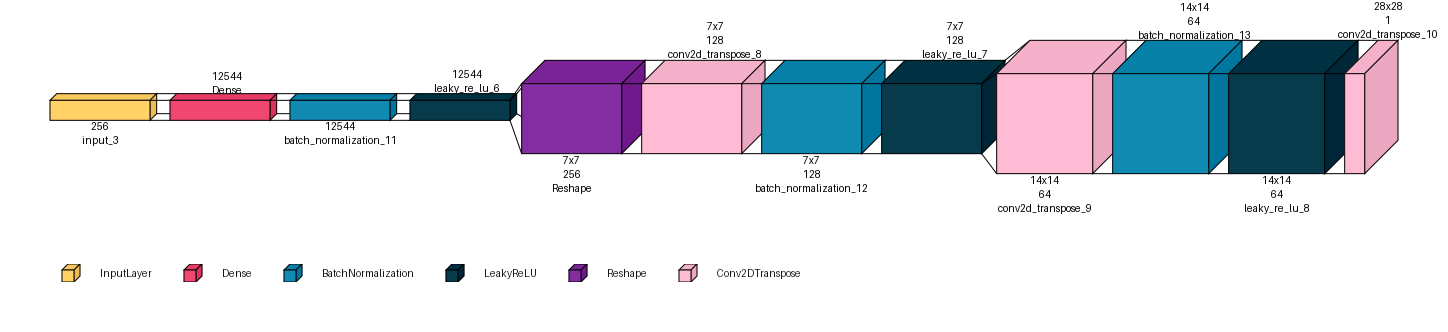
\includegraphics[width=.9\textwidth]{abb/netron_network_archs/define_vanilla_mnist_gen.png}
    \caption{Depiction of the generator used in the deep convolutional GAN dependent experiments. Used to train a generator and create fake image data based on the MNIST dataset.}
    \label{fig:figure_gen_arch_vanilla_mnist}
\end{figure}

\begin{figure}[htbp]
    \centering
    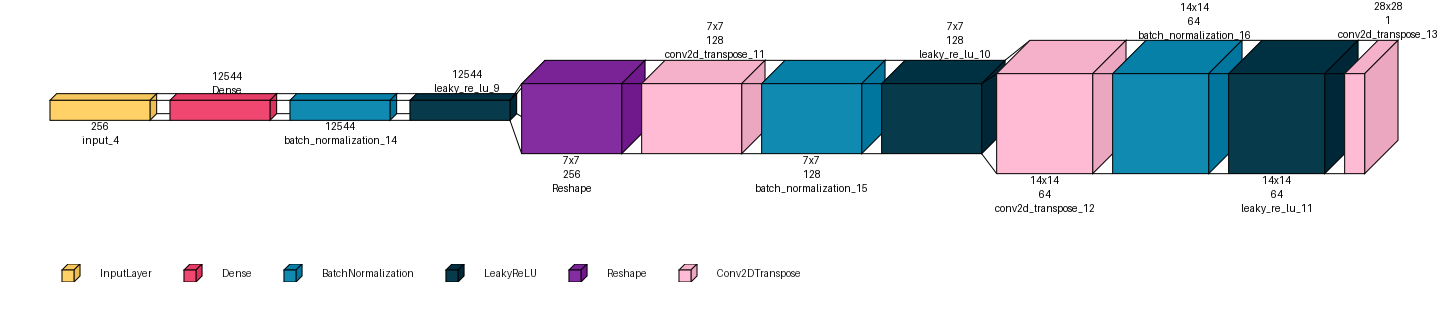
\includegraphics[width=.9\textwidth]{abb/netron_network_archs/define_vanilla_fashion_mnist_gen.png}
    \caption{Depiction of the generator used in the deep convolutional GAN dependent experiments. Used to train a generator and create fake image data based on the Fashion-MNIST dataset.}
    \label{fig:figure_gen_arch_vanilla_fashion}
\end{figure}

\begin{figure}[htbp]
    \centering
    \vspace{-2em}
    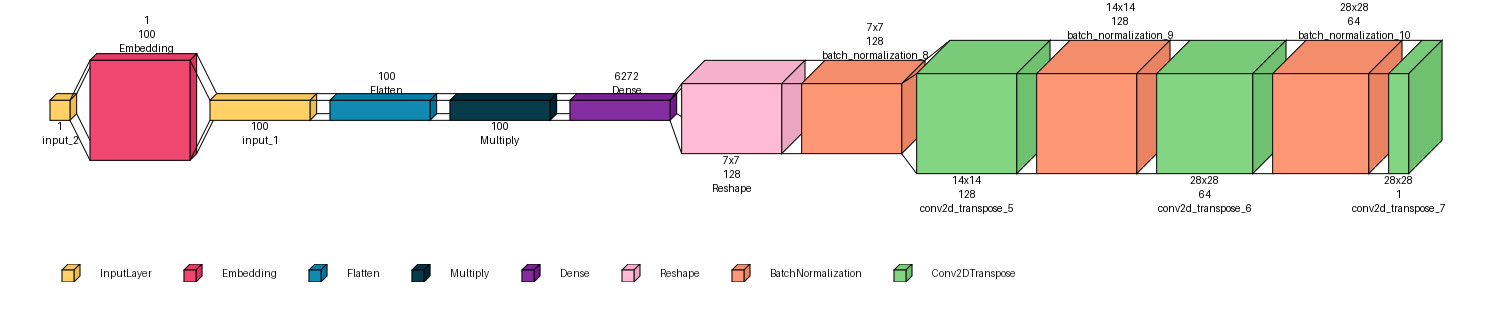
\includegraphics[width=.9\textwidth]{abb/netron_network_archs/define_conditional_mnists_gen.png}
    \caption{Depiction of the generator used in the Conditional GAN dependent experiments. Used to train a generator and create fake image data based on the MNIST and Fashion-MNIST datasets.}
    \label{fig:figure_gen_arch_conditional}
\end{figure}

\begin{figure}[htbp]
    \centering
    \vspace{-2em}
    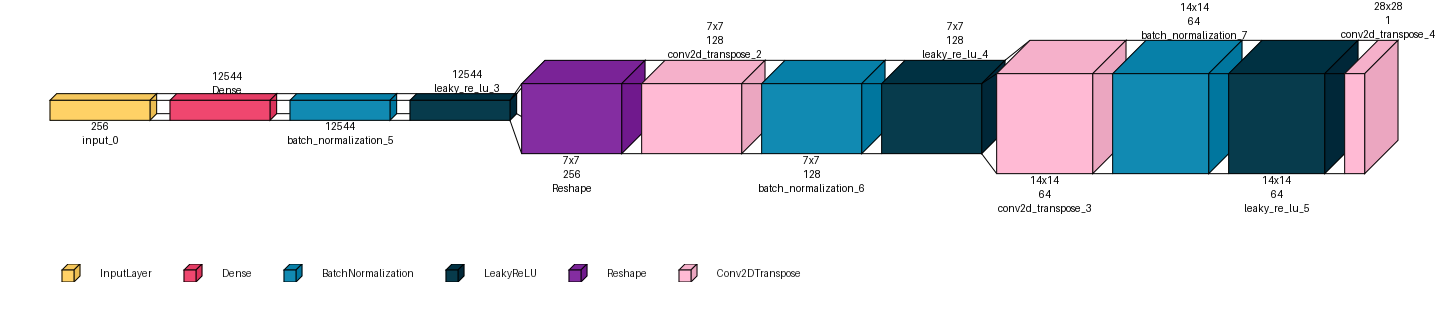
\includegraphics[width=.9\textwidth]{abb/netron_network_archs/define_madgan_mnists_gen.png}
    \caption{Depiction of the generators used in the MADGAN dependent experiments. Used to train a generator and create fake image data based on the MNIST and Fashion-MNIST datasets.}
    \label{fig:figure_gen_arch_madgan}
\end{figure}

\begin{figure}[htbp]
    \centering
    \vspace{-2em}
    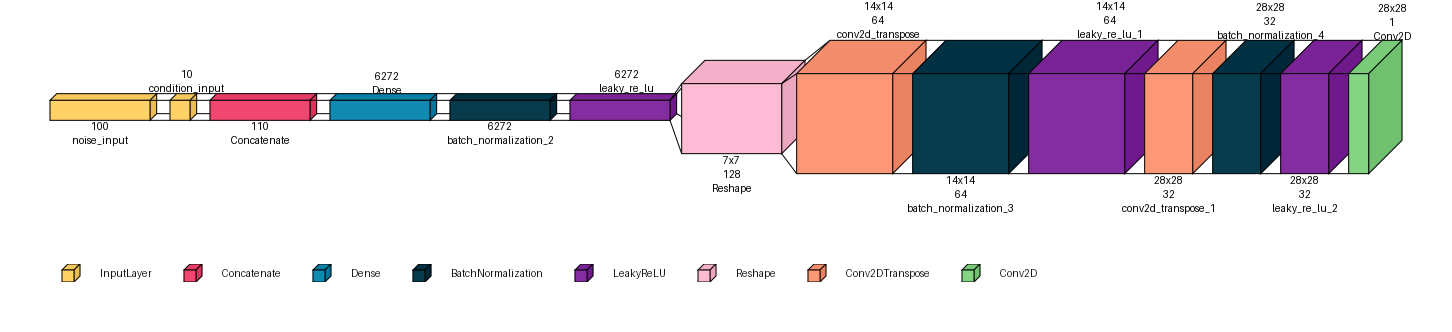
\includegraphics[width=.9\textwidth]{abb/netron_network_archs/define_cmadgan_mnists_gen.png}
    \caption{Depiction of the generators used in the cMADGAN dependent experiments. Used to train a generator and create fake image data based on the MNIST and Fashion-MNIST datasets.}
    \label{fig:figure_gen_arch_cmadgan}
\end{figure}
\newpage


\subsubsection{Discriminator Model Architectures}\label{appendix_discriminator_architectures}
The graphical representations of the network architectures are created with the tool \textit{visual keras}, by Paul Gavrikov (\cite{Gavrikov2020VisualKeras}).

\begin{figure}[htbp]
    \centering
    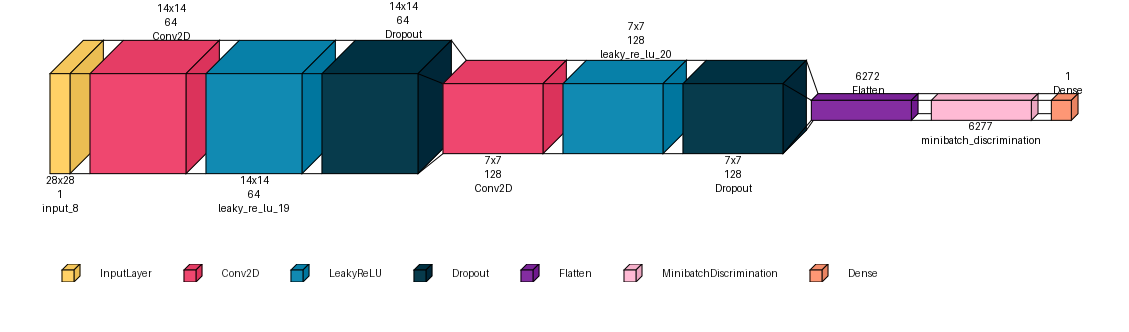
\includegraphics[width=.9\textwidth]{abb/netron_network_archs/define_vanilla_mnist_disc.png}
    \caption{Depiction of the discriminator used in the deep convolutional GAN dependent experiments. Used to train a generator based on the MNIST dataset.}
    \label{fig:figure_disc_arch_vanilla_mnist}
\end{figure}

\begin{figure}[htbp]
    \centering
    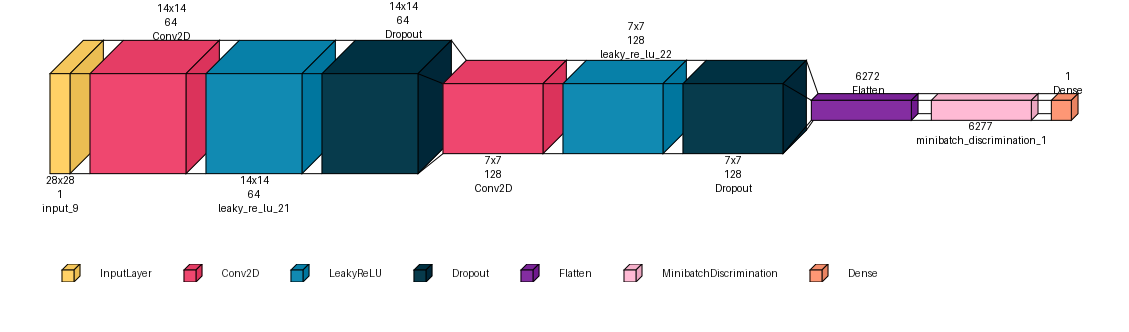
\includegraphics[width=.9\textwidth]{abb/netron_network_archs/define_vanilla_fashion_mnist_disc.png}
    \caption{Depiction of the discriminator used in the deep convolutional GAN dependent experiments. Used to train a generator based on the Fashion-MNIST dataset.}
    \label{fig:figure_disc_arch_vanilla_fashion}
\end{figure}

\begin{figure}[htbp]
    \centering
    \vspace{-2em}
    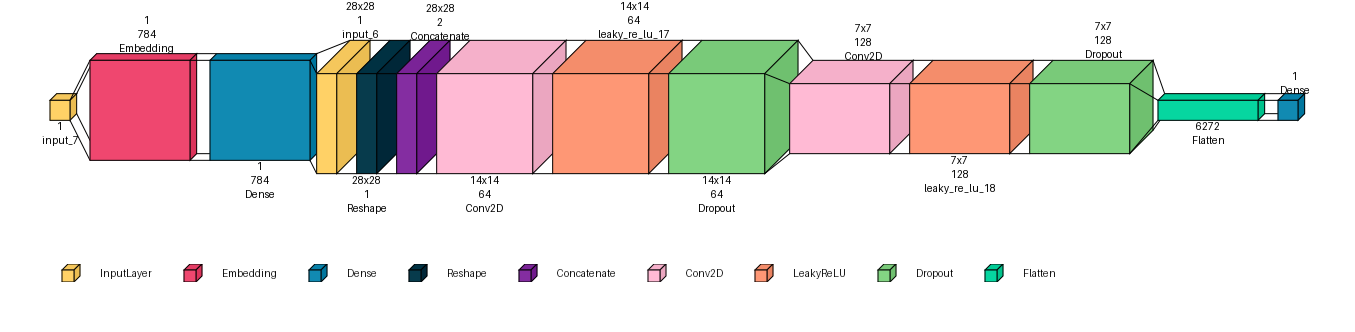
\includegraphics[width=.9\textwidth]{abb/netron_network_archs/define_conditional_mnists_disc.png}
    \caption{Depiction of the discriminator used in the Conditional GAN dependent experiments. Used to train a generator based on the MNIST and Fashion-MNIST datasets.}
    \label{fig:figure_disc_arch_conditional}
\end{figure}

\begin{figure}[htbp]
    \centering
    \vspace{-2em}
    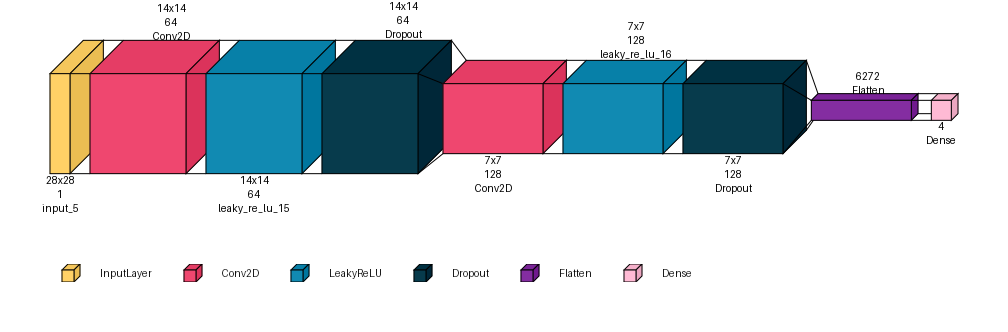
\includegraphics[width=.9\textwidth]{abb/netron_network_archs/define_madgan_mnists_disc.png}
    \caption{Depiction of the discriminator used in the MADGAN dependent experiments. Used to train a generator based on the MNIST and Fashion-MNIST datasets.}
    \label{fig:figure_disc_arch_madgan}
\end{figure}

\begin{figure}[htbp]
    \centering
    \vspace{-2em}
    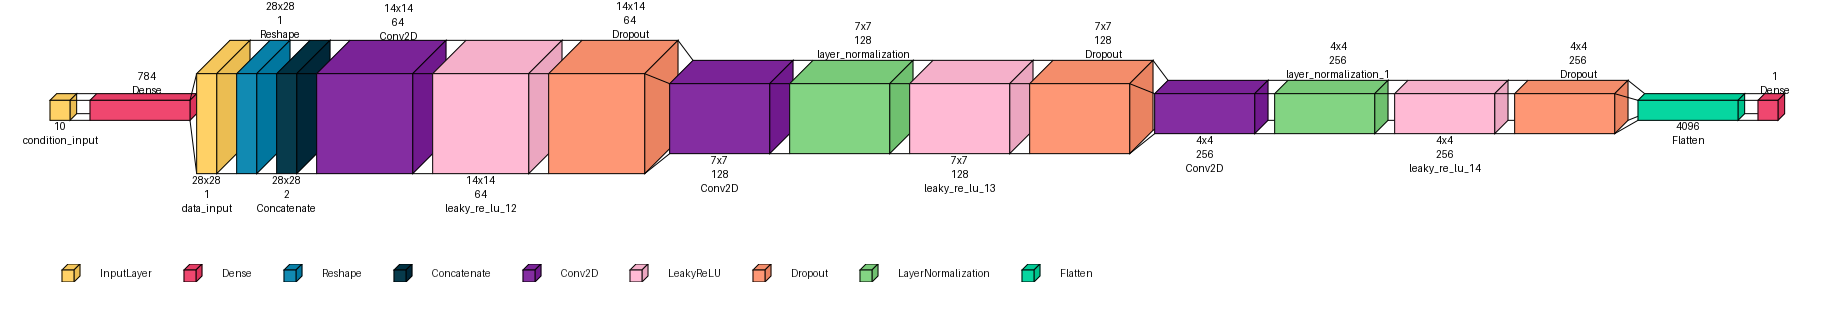
\includegraphics[width=.9\textwidth]{abb/netron_network_archs/define_cmadgan_mnists_disc.png}
    \caption{Depiction of the discriminator used in the cMADGAN dependent experiments. Used to train a generator based on the MNIST and Fashion-MNIST datasets.}
    \label{fig:figure_disc_arch_cmadgan}
\end{figure}

\newpage


\subsection{FID and Inception Scores from MADGAN Architectures}

\subsubsection{MADGAN MNIST}
\begin{table}[H]
    \centering
    \begin{tabular}{|c|c|c|c|c|}
    \hline
    N Generators & Index & FID & IS & IS-std \\
    \hline
    \textit{Baseline} & & $-0.004$ & $2.549$ & $0.036$ \\
    \specialrule{.1em}{.05em}{.05em}
    & 0 &        $23.597$ & $2.519$ & $0.050$ \\
    3 & 1 &      $22.682$ & $2.506$ & $0.027$ \\
    & 2 &        $23.252$ & $2.509$ & $0.045$ \\
    \hline
    & 0 &        $23.304$ & $2.467$ & $0.030$ \\
    & 1 &        $22.020$ & $2.446$ & $0.040$ \\
    5 & 2 &      $23.076$ & $2.497$ & $0.046$ \\
    & 3 &        $22.265$ & $2.467$ & $0.060$ \\
    & 4 &        $22.614$ & $2.479$ & $0.045$ \\
    \hline
    & 0 &        $22.487$ & $2.513$ & $0.031$ \\
    & 1 &        $21.076$ & $\mathbf{2.548}$ & $0.087$ \\
    & 2 &        $20.941$ & $2.530$ & $0.056$ \\
    7 & 3 &      $22.250$ & $2.520$ & $0.035$ \\
    & 4 &        $21.557$ & $2.530$ & $0.051$ \\
    & 5 &        $21.297$ & $2.545$ & $0.035$ \\
    & 6 &        $21.582$ & $2.541$ & $0.059$ \\
    \hline
    & 0 &        $21.338$ & $2.456$ & $0.045$ \\
    & 1 &        $20.872$ & $2.462$ & $0.040$ \\
    & 2 &        $20.680$ & $2.477$ & $0.028$ \\
    & 3 &        $21.315$ & $2.470$ & $0.030$ \\
    10 & 4 &     $21.158$ & $2.484$ & $0.027$ \\
    & 5 &        $20.655$ & $2.473$ & $0.037$ \\
    & 6 &        $21.090$ & $2.452$ & $0.039$ \\
    & 7 &        $20.689$ & $2.508$ & $0.048$ \\
    & 8 &        $21.471$ & $2.480$ & $0.044$ \\
    & 9 &        $\mathbf{20.459}$ & $2.477$ & $0.036$ \\
    \hline
\end{tabular}
\caption{Effect of varying the number of generators ($N=3, 5, 7, 10$) in the MADGAN model on FID and Inception Score (IS $\pm$ Std. Dev) for the \textbf{MNIST} dataset. Results for each generator index are presented alongside baseline metrics.}
\label{tab:app_madgan_mnist_fid_is}
\end{table}
\newpage


\subsubsection{MADGAN Fashion-MNIST}
\begin{table}[H]
    \centering
    \begin{tabular}{|c|c|c|c|c|}
    \hline
    N Generators & Index & FID & IS & IS-std \\
    \hline
    \textit{Baseline} & & $-0.004$ & $4.723$ & $0.056$ \\
    \specialrule{.1em}{.05em}{.05em}
    & 0 &       $26.086$ & $4.463$ & $0.103$ \\
    3 & 1 &     $25.884$ & $4.487$ & $0.099$ \\
    & 2 &       $26.637$ & $4.538$ & $0.094$ \\
    \hline
    & 0 &       $23.393$ & $4.467$ & $0.119$ \\
    & 1 &       $24.756$ & $4.520$ & $0.107$ \\
    5 & 2 &     $25.663$ & $4.506$ & $0.123$ \\
    & 3 &       $23.614$ & $4.487$ & $0.082$ \\
    & 4 &       $23.665$ & $4.504$ & $0.061$ \\
    \hline
    & 0 &       $22.370$ & $4.558$ & $0.111$ \\
    & 1 &       $21.838$ & $4.536$ & $0.087$ \\
    & 2 &       $21.923$ & $4.508$ & $0.101$ \\
    7 & 3 &     $25.403$ & $4.517$ & $0.112$ \\
    & 4 &       $31.493$ & $4.372$ & $0.087$ \\
    & 5 &       $22.158$ & $4.595$ & $0.075$ \\
    & 6 &       $21.942$ & $4.577$ & $0.087$ \\
    \hline
    & 0 &       $22.454$ & $4.534$ & $0.117$ \\
    & 1 &       $21.914$ & $4.524$ & $0.121$ \\
    & 2 &       $21.327$ & $4.494$ & $0.089$ \\
    & 3 &       $21.630$ & $4.455$ & $0.063$ \\
    10 & 4 &    $\mathbf{20.851}$ & $\mathbf{4.575}$ & $0.097$ \\
    & 5 &       $21.268$ & $4.561$ & $0.048$ \\
    & 6 &       $22.324$ & $4.566$ & $0.127$ \\
    & 7 &       $21.633$ & $4.542$ & $0.084$ \\
    & 8 &       $21.503$ & $4.533$ & $0.127$ \\
    & 9 &       $20.963$ & $4.552$ & $0.100$ \\
    \hline
    \end{tabular}
    \caption{Effect of varying the number of generators ($N=3, 5, 7, 10$) in the MADGAN model on FID and Inception Score (IS $\pm$ Std. Dev) for the \textbf{Fashion-MNIST} dataset. Results for each generator index are presented alongside baseline metrics.}
    \label{tab:madgan_fasion_mnist_fid_is}
\end{table}
\newpage

\subsubsection{cMADGAN MNIST}
\begin{table}[H]
    \centering
    \begin{tabular}{|c|c|c|c|c|}
    \hline
    N Generators & Index & FID & IS & IS-std \\
    \hline
    \textit{Baseline} & & $-0.004$ & $2.549$ & $0.036$ \\
    \specialrule{.1em}{.05em}{.05em}
    & 0 &       $30.105$ & $\mathbf{2.494}$ & $0.034$ \\
    3 & 1 &     $23.875$ & $2.317$ & $0.041$ \\
    & 2 &       $\mathbf{22.753}$ & $2.384$ & $0.032$ \\
    \hline
    & 0 &       $37.638$ & $2.460$ & $0.039$ \\
    & 1 &       $26.614$ & $2.378$ & $0.052$ \\
    5 & 2 &     $26.739$ & $2.356$ & $0.025$ \\
    & 3 &       $27.642$ & $2.309$ & $0.034$ \\
    & 4 &       $26.722$ & $2.246$ & $0.043$ \\
    \hline
    & 0 &       $23.141$ & $2.418$ & $0.037$ \\a
    & 1 &       $28.071$ & $2.363$ & $0.036$ \\
    & 2 &       $33.490$ & $2.340$ & $0.033$ \\
    7 & 3 &     $28.333$ & $2.347$ & $0.031$ \\
    & 4 &       $35.599$ & $2.296$ & $0.050$ \\
    & 5 &       $36.075$ & $2.389$ & $0.047$ \\
    & 6 &       $29.807$ & $2.326$ & $0.036$ \\
    \hline
    & 0 &       $108.079$ & $2.076$ & $0.011$ \\
    & 1 &       $82.478$ & $2.250$ & $0.022$ \\
    & 2 &       $153.369$ & $2.124$ & $0.023$ \\
    & 3 &       $126.574$ & $1.846$ & $0.005$ \\
    10 & 4 &    $110.012$ & $2.005$ & $0.013$ \\
    & 5 &       $130.054$ & $1.861$ & $0.009$ \\
    & 6 &       $103.016$ & $2.010$ & $0.011$ \\
    & 7 &       $74.926$ & $2.383$ & $0.035$ \\
    & 8 &       $110.265$ & $2.086$ & $0.014$ \\
    & 9 &       $106.762$ & $1.975$ & $0.033$ \\
    \hline
    \end{tabular}
    \caption{Effect of varying the number of generators ($N=3, 5, 7, 10$) in the cMADGAN model on FID and Inception Score (IS $\pm$ Std. Dev) for the \textbf{MNIST} dataset. Results for each generator index are presented alongside baseline metrics.}
    \label{tab:cmadgan_mnist_fid_is}
\end{table}
\newpage

\subsubsection{cMADGAN Fashion-MNIST}
\begin{table}[H]
    \centering
    \begin{tabular}{|c|c|c|c|c|}
    \hline
    N Generators & Index & FID & IS & IS-std \\
    \hline
    \textit{Baseline} & & $-0.004$ & $4.723$ & $0.056$ \\
    \specialrule{.1em}{.05em}{.05em}
    & 0 &       $25.874$ & $4.750$ & $0.132$ \\
    3 & 1 &     $27.235$ & $4.068$ & $0.090$ \\
    & 2 &       $\mathbf{23.556}$ & $\mathbf{5.049}$ & $0.093$ \\
    \hline
    & 0 &       $170.120$ & $2.938$ & $0.020$ \\
    & 1 &       $167.446$ & $3.430$ & $0.052$ \\
    5 & 2 &     $221.934$ & $3.325$ & $0.032$ \\
    & 3 &       $187.293$ & $3.269$ & $0.029$ \\
    & 4 &       $53.616$ & $3.770$ & $0.057$ \\
    \hline
    & 0 &       $156.601$ & $2.392$ & $0.016$ \\
    & 1 &       $172.054$ & $3.325$ & $0.033$ \\
    & 2 &       $171.505$ & $2.754$ & $0.024$ \\
    7 & 3 &     $97.514$ & $3.273$ & $0.058$ \\
    & 4 &       $155.474$ & $3.157$ & $0.063$ \\
    & 5 &       $151.494$ & $2.623$ & $0.018$ \\
    & 6 &       $174.161$ & $2.976$ & $0.028$ \\
    \hline
    & 0 &       $147.670$ & $3.650$ & $0.037$ \\
    & 1 &       $167.407$ & $2.816$ & $0.026$ \\
    & 2 &       $109.349$ & $3.914$ & $0.068$ \\
    & 3 &       $160.305$ & $3.674$ & $0.040$ \\
    10 & 4 &    $181.778$ & $2.961$ & $0.023$ \\
    & 5 &       $154.633$ & $3.297$ & $0.022$ \\
    & 6 &       $166.511$ & $2.759$ & $0.034$ \\
    & 7 &       $156.135$ & $3.173$ & $0.027$ \\
    & 8 &       $155.758$ & $3.853$ & $0.036$ \\
    & 9 &       $191.126$ & $3.073$ & $0.034$ \\
    \hline
    \end{tabular}
    \caption{Effect of varying the number of generators ($N=3, 5, 7, 10$) in the cMADGAN model on FID and Inception Score (IS $\pm$ Std. Dev) for the \textbf{Fashion-MNIST} dataset. Results for each generator index are presented alongside baseline metrics.}
    \label{tab:cmadgan_fashnion_mnist_fid_is}
\end{table}
\newpage


\subsubsection{DCGAN MNIST}
\begin{table}[H]
    \centering
    \begin{tabular}{|c|c|c|c|}
    \hline
    N Generators & FID & IS & IS-std \\
    \hline
    \textit{Baseline} & $-0.004$ & $2.549$ & $0.036$ \\
    \specialrule{.1em}{.05em}{.05em}
    1 & $122.097$ & $2.611$ & $0.056$ \\
    \hline
    \end{tabular}
    \caption{FID and Inception Score (Mean $\pm$ Std. Dev) for a single DCGAN generator ($N=1$) trained on the \textbf{MNIST} dataset. Baseline scores are included for reference.}
    \label{tab:dcgan_mnist_n1}
\end{table}

\subsubsection{DCGAN Fashion-MNIST}
\begin{table}[H]
    \centering
    \begin{tabular}{|c|c|c|c|}
    \hline
    N Generators & FID & IS & IS-std \\
    \hline
    \textit{Baseline} & $-0.004$ & $4.723$ & $0.056$ \\
    \specialrule{.1em}{.05em}{.05em}
    1 & $123.349$ & $3.573$ & $0.117$ \\
    \hline
    \end{tabular}
    \caption{FID and Inception Score (Mean $\pm$ Std. Dev) for a single DCGAN generator ($N=1$) trained on the \textbf{Fashion-MNIST} dataset. Baseline scores are included for reference.}
    \label{tab:dcgan_fashion_mnist_n1}
\end{table}

\subsubsection{Conditional MNIST}
\begin{table}[H]
    \centering
    \begin{tabular}{|c|c|c|c|}
    \hline
    N Generators & FID & IS & IS-std \\
    \hline
    \textit{Baseline} & $-0.004$ & $2.549$ & $0.036$ \\
    \specialrule{.1em}{.05em}{.05em}
    1 & $28.721$ & $2.553$ & $0.022$ \\
    \hline
    \end{tabular}
    \caption{FID and Inception Score (Mean $\pm$ Std. Dev) for a single Conditional GAN generator ($N=1$) trained on the \textbf{MNIST} dataset. Baseline scores are included for reference.}
    \label{tab:cgan_mnist_n1}
\end{table}

\subsubsection{Conditional Fashion-MNIST}
\begin{table}[H]
    \centering
    \begin{tabular}{|c|c|c|c|}
    \hline
    N Generators & FID & IS & IS-std \\
    \hline
    \textit{Baseline} & $-0.004$ & $4.723$ & $0.056$ \\
    \specialrule{.1em}{.05em}{.05em}
    1 & $25.560$ & $4.210$ & $0.099$ \\
    \hline
    \end{tabular}
    \caption{FID and Inception Score (Mean $\pm$ Std. Dev) for a single Conditional GAN generator ($N=1$) trained on the \textbf{Fashion-MNIST} dataset. Baseline scores are included for reference.}
    \label{tab:cgan_fashion_mnist_n1}
\end{table}

\newpage

\subsection{Stratified Classifier Performances and Graphs} \label{app_strat_class_performance}

\subsubsection{Dataset: MNIST, Architecture: MADGAN}\label{app_strat_class_performance_madgan_mnist}
% LaTeX Metrics Table for Expansion Experiment: - Metric: val_f1_score - Target Gen Group: 3
\noindent\textbf{Expansion Experiment: K=3}
\begin{figure}[htbp]
	\centering
	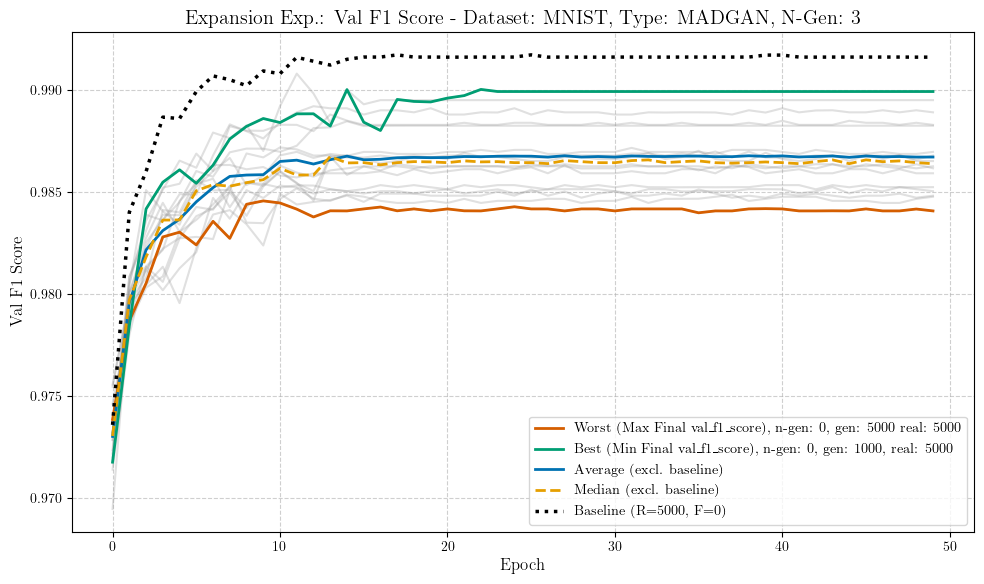
\includegraphics[width=.85\textwidth]{abb/strat_classifier_performance/MNIST_STRATIFIED_CLASSIFIERS_MADGAN_NEW/expansion_experiments/val_f1_score_MADGAN_MNIST_n_gen_3_all.png}
	\label{fig:app_strat_class_performance_expansion_exp._val_f1_score_3}
\end{figure}
\begin{table}[H]
	\vspace{-1.5em}
	\centering
	\begin{tabular}{|c|c|c|c|}
		\hline
		Run Type & Experiment & Val F1 \\ \hline
		best & \(G_{3, 0}\), R:5000, F:1000 & $0.9899$\\ \hline
		worst & \(G_{3, 0}\), R:5000, F:5000 & $0.9841$\\ \hline
		median & G (K=3) & $0.9864$\\ \hline
		average & G (K=3) & $0.9867$
		\\ \hline
	\end{tabular}
\end{table}
% End LaTeX Table for Expansion Experiment:
% LaTeX Metrics Table for Replacement Experiment: - Metric: val_f1_score - Target Gen Group: 3
\noindent\textbf{Replacement Experiment: K=3}
\begin{figure}[htbp]
	\centering
	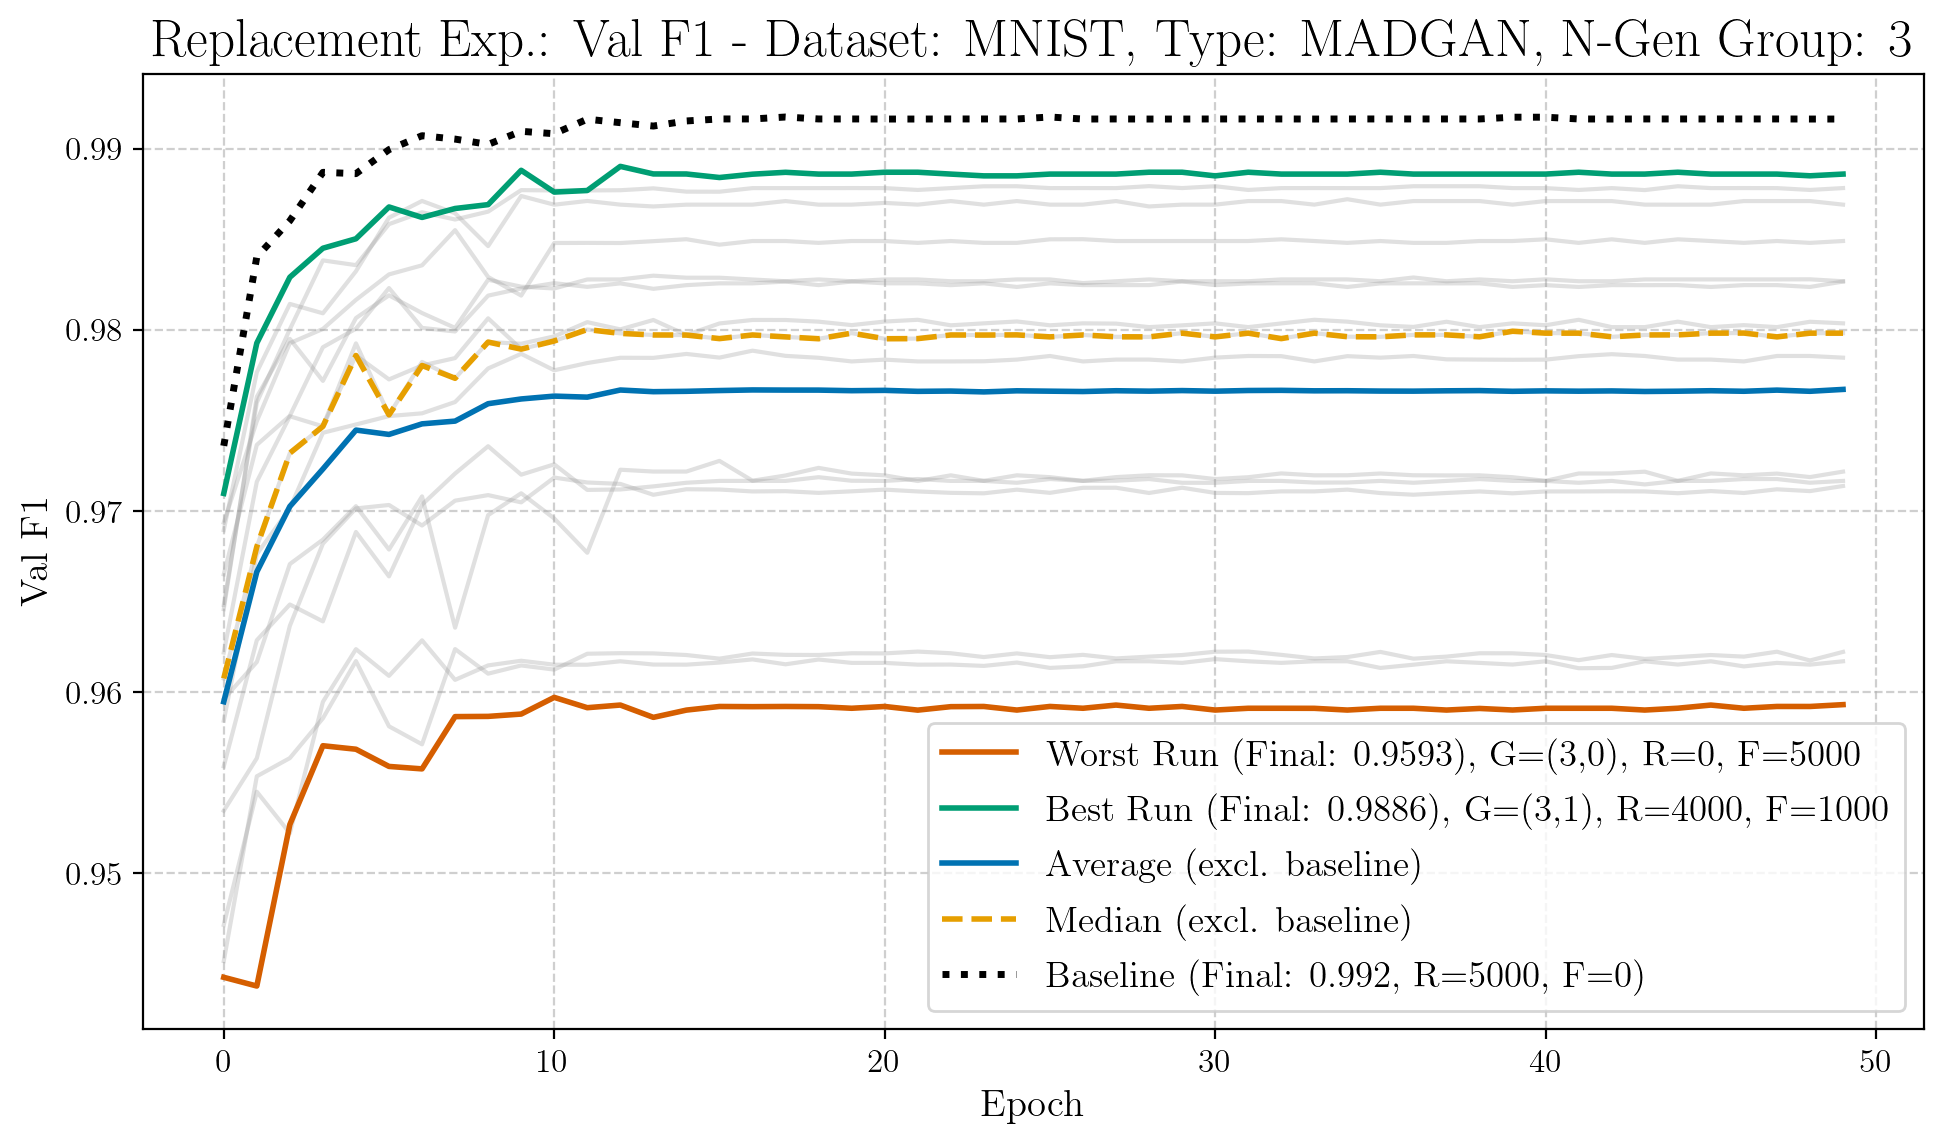
\includegraphics[width=.85\textwidth]{abb/strat_classifier_performance/MNIST_STRATIFIED_CLASSIFIERS_MADGAN_NEW/replacement_experiments/val_f1_score_MADGAN_MNIST_n_gen_3_all.png}
	\label{fig:app_strat_class_performance_replacement_exp._val_f1_score_3}
\end{figure}
\begin{table}[H]
	\vspace{-1.5em}
	\centering
	\begin{tabular}{|c|c|c|c|}
		\hline
		Run Type & Experiment & Val F1 \\ \hline
		best & \(G_{3, 1}\), R:4000, F:1000 & $0.9886$\\ \hline
		worst & \(G_{3, 0}\), R:0, F:5000 & $0.9593$\\ \hline
		median & G (K=3) & $0.9798$\\ \hline
		average & G (K=3) & $0.9767$
		\\ \hline
	\end{tabular}
\end{table}
% End LaTeX Table for Replacement Experiment:
\newpage
% LaTeX Metrics Table for Expansion Experiment: - Metric: val_f1_score - Target Gen Group: 5
\noindent\textbf{Expansion Experiment: K=5}
\begin{figure}[htbp]
	\centering
	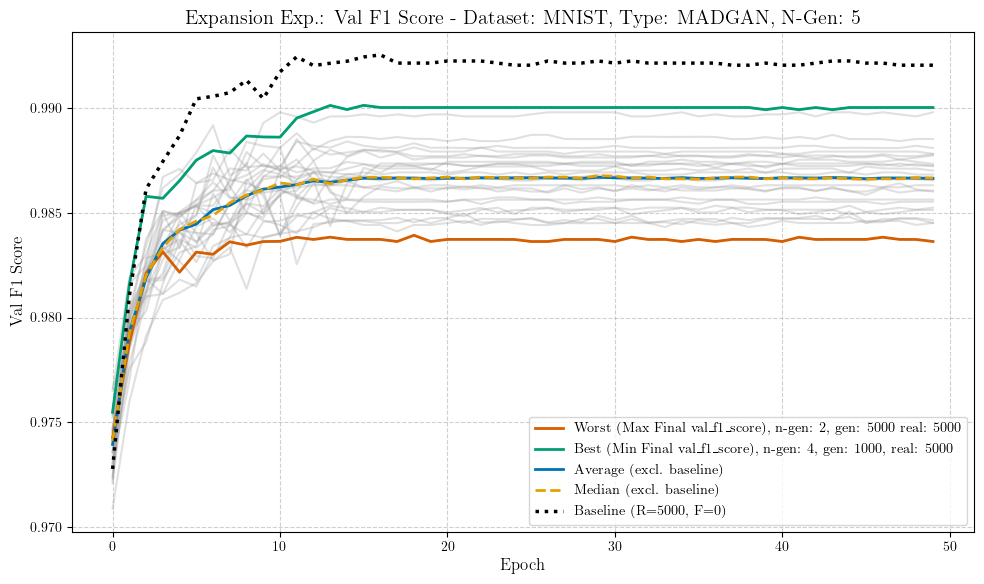
\includegraphics[width=.85\textwidth]{abb/strat_classifier_performance/MNIST_STRATIFIED_CLASSIFIERS_MADGAN_NEW/expansion_experiments/val_f1_score_MADGAN_MNIST_n_gen_5_all.png}
	\label{fig:app_strat_class_performance_expansion_exp._val_f1_score_5}
\end{figure}
\begin{table}[H]
	\vspace{-1em}
	\centering
	\begin{tabular}{|c|c|c|c|}
		\hline
		Run Type & Experiment & Val F1 \\ \hline
		best & \(G_{5, 4}\), R:5000, F:1000 & $0.9900$\\ \hline
		worst & \(G_{5, 2}\), R:5000, F:5000 & $0.9836$\\ \hline
		median & G (K=5) & $0.9867$\\ \hline
		average & G (K=5) & $0.9866$
		\\ \hline
	\end{tabular}
\end{table}
% End LaTeX Table for Expansion Experiment:
% LaTeX Metrics Table for Replacement Experiment: - Metric: val_f1_score - Target Gen Group: 5
\noindent\textbf{Replacement Experiment: K=5}
\begin{figure}[htbp]
	\centering
	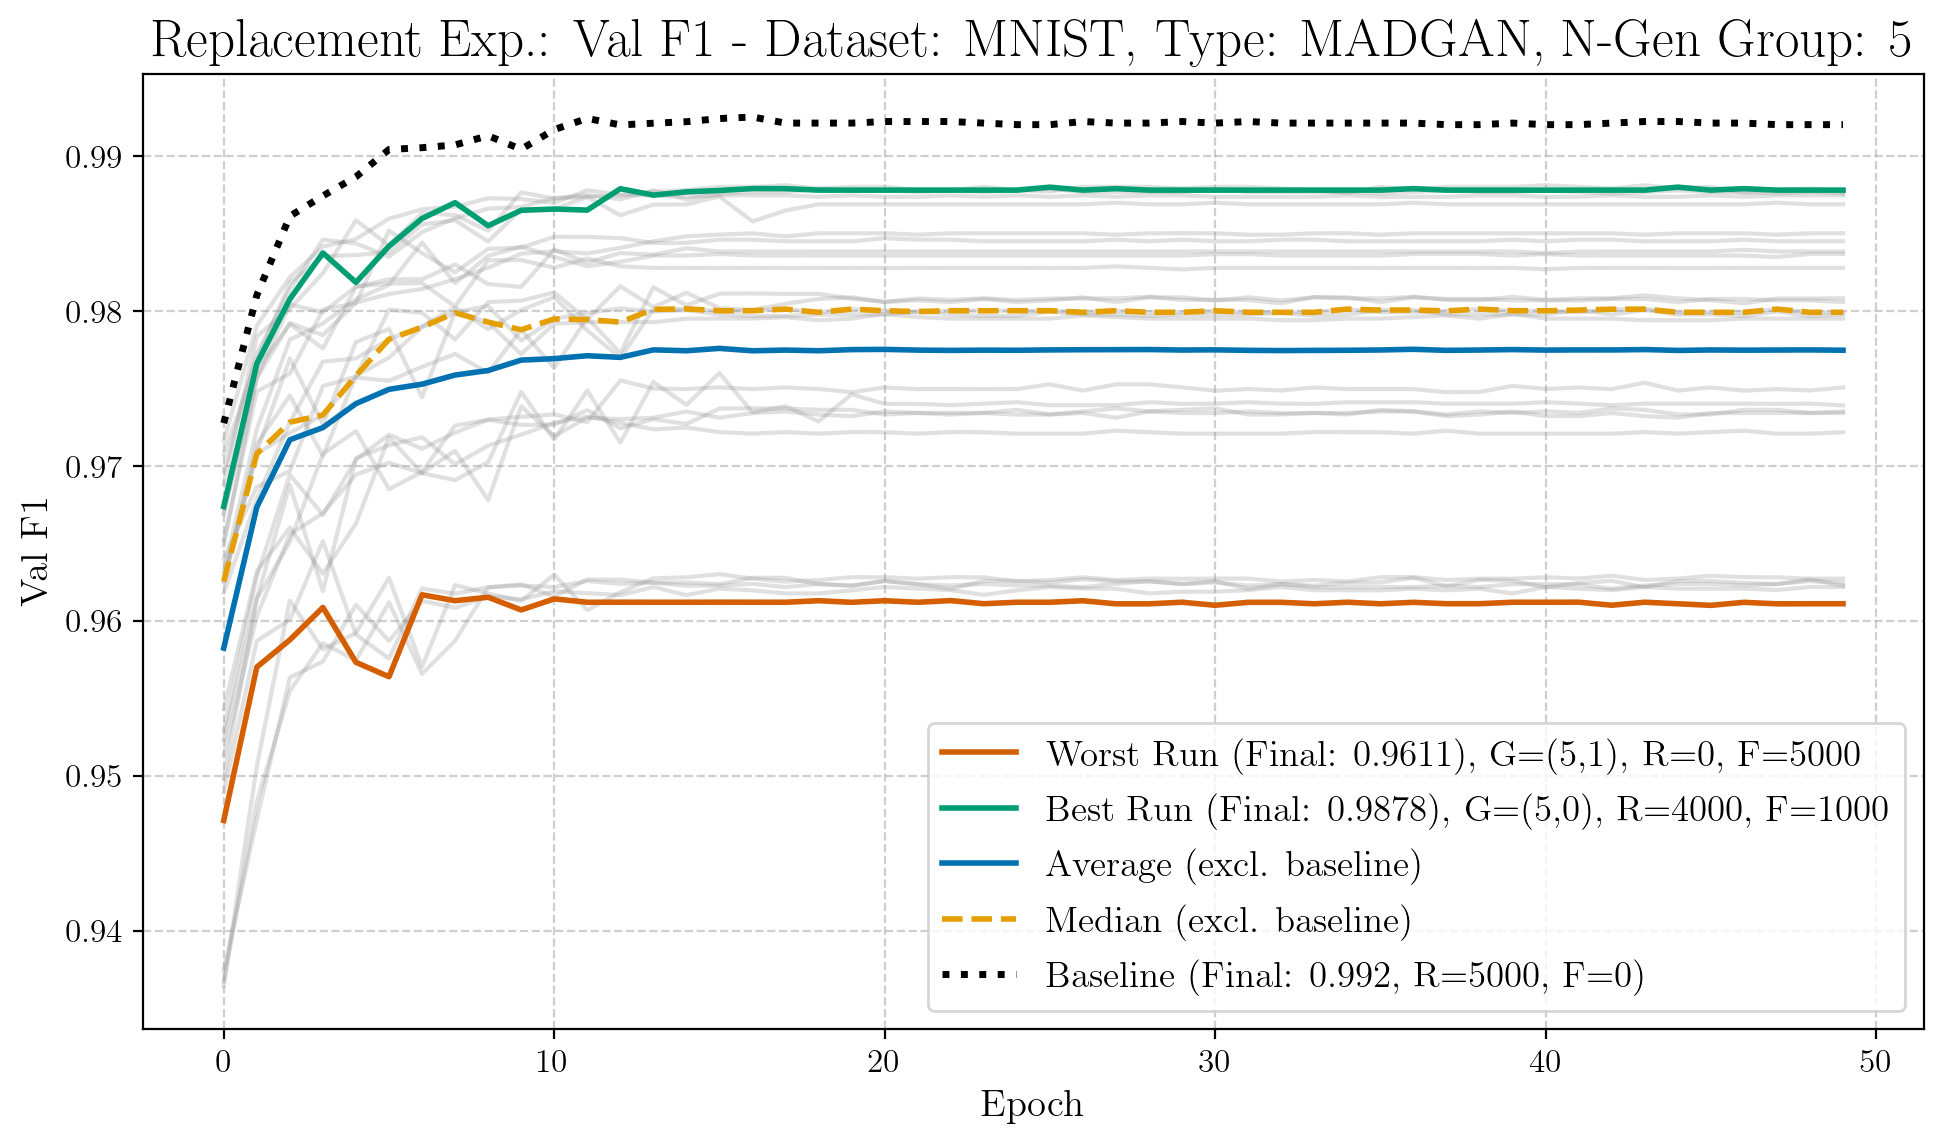
\includegraphics[width=.85\textwidth]{abb/strat_classifier_performance/MNIST_STRATIFIED_CLASSIFIERS_MADGAN_NEW/replacement_experiments/val_f1_score_MADGAN_MNIST_n_gen_5_all.png}
	\label{fig:app_strat_class_performance_replacement_exp._val_f1_score_5}
\end{figure}
\begin{table}[H]
	\vspace{-1em}
	\centering
	\begin{tabular}{|c|c|c|c|}
		\hline
		Run Type & Experiment & Val F1 \\ \hline
		best & \(G_{5, 0}\), R:4000, F:1000 & $0.9878$\\ \hline
		worst & \(G_{5, 1}\), R:0, F:5000 & $0.9611$\\ \hline
		median & G (K=5) & $0.9799$\\ \hline
		average & G (K=5) & $0.9775$
		\\ \hline
	\end{tabular}
\end{table}
% End LaTeX Table for Replacement Experiment:
\newpage
% LaTeX Metrics Table for Expansion Experiment: - Metric: val_f1_score - Target Gen Group: 7
\noindent\textbf{Expansion Experiment: K=7}
\begin{figure}[htbp]
	\centering
	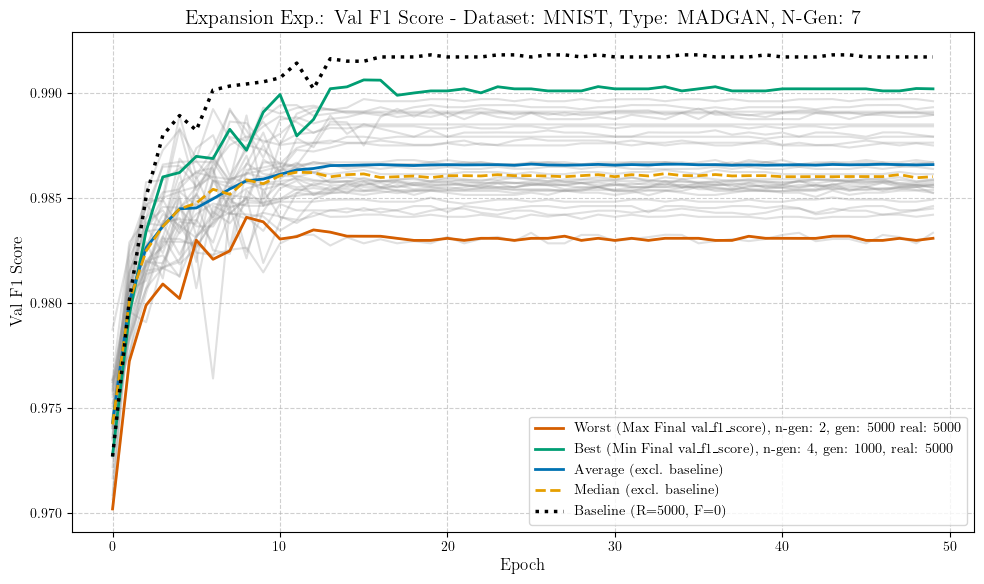
\includegraphics[width=.85\textwidth]{abb/strat_classifier_performance/MNIST_STRATIFIED_CLASSIFIERS_MADGAN_NEW/expansion_experiments/val_f1_score_MADGAN_MNIST_n_gen_7_all.png}
	\label{fig:app_strat_class_performance_expansion_exp._val_f1_score_7}
\end{figure}
\begin{table}[H]
	\vspace{-1em}
	\centering
	\begin{tabular}{|c|c|c|c|}
		\hline
		Run Type & Experiment & Val F1 \\ \hline
		best & \(G_{7, 4}\), R:5000, F:1000 & $0.9902$\\ \hline
		worst & \(G_{7, 2}\), R:5000, F:5000 & $0.9831$\\ \hline
		median & G (K=7) & $0.9860$\\ \hline
		average & G (K=7) & $0.9866$
		\\ \hline
	\end{tabular}
\end{table}
% End LaTeX Table for Expansion Experiment:
% LaTeX Metrics Table for Replacement Experiment: - Metric: val_f1_score - Target Gen Group: 7
\noindent\textbf{Replacement Experiment: K=7}
\begin{figure}[htbp]
	\centering
	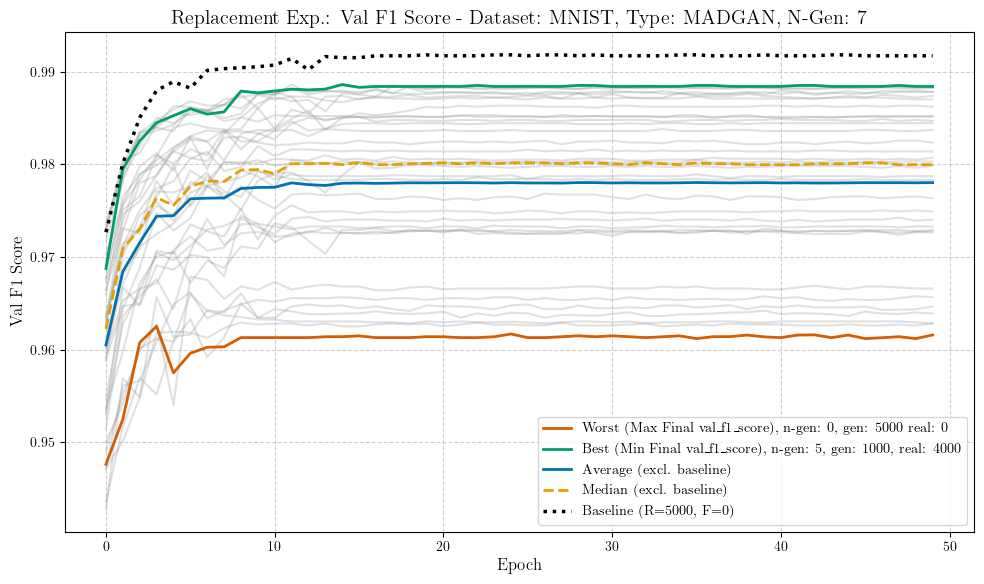
\includegraphics[width=.85\textwidth]{abb/strat_classifier_performance/MNIST_STRATIFIED_CLASSIFIERS_MADGAN_NEW/replacement_experiments/val_f1_score_MADGAN_MNIST_n_gen_7_all.png}
	\label{fig:app_strat_class_performance_replacement_exp._val_f1_score_7}
\end{figure}
\begin{table}[H]
	\vspace{-1em}
	\centering
	\begin{tabular}{|c|c|c|c|}
		\hline
		Run Type & Experiment & Val F1 \\ \hline
		best & \(G_{7, 5}\), R:4000, F:1000 & $0.9884$\\ \hline
		worst & \(G_{7, 0}\), R:0, F:5000 & $0.9616$\\ \hline
		median & G (K=7) & $0.9800$\\ \hline
		average & G (K=7) & $0.9780$
		\\ \hline
	\end{tabular}
\end{table}
% End LaTeX Table for Replacement Experiment:
\newpage
% LaTeX Metrics Table for Expansion Experiment: - Metric: val_f1_score - Target Gen Group: 10
\noindent\textbf{Expansion Experiment: K=10}
\begin{figure}[htbp]
	\centering
	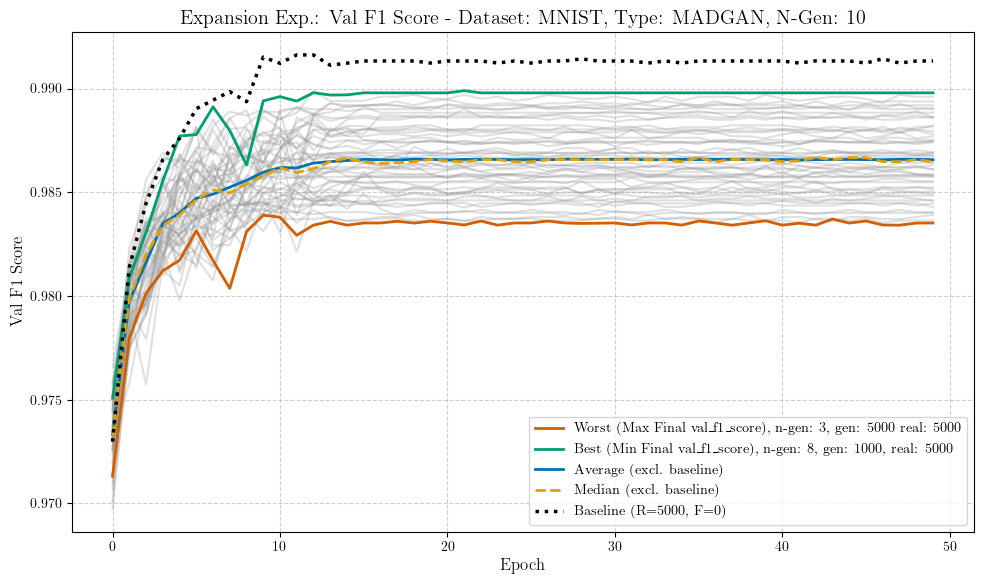
\includegraphics[width=.85\textwidth]{abb/strat_classifier_performance/MNIST_STRATIFIED_CLASSIFIERS_MADGAN_NEW/expansion_experiments/val_f1_score_MADGAN_MNIST_n_gen_10_all.png}
	\label{fig:app_strat_class_performance_expansion_exp._val_f1_score_10}
\end{figure}
\begin{table}[H]
	\vspace{-1em}
	\centering
	\begin{tabular}{|c|c|c|c|}
		\hline
		Run Type & Experiment & Val F1 \\ \hline
		best & \(G_{10, 8}\), R:5000, F:1000 & $0.9898$\\ \hline
		worst & \(G_{10, 3}\), R:5000, F:5000 & $0.9835$\\ \hline
		median & G (K=10) & $0.9865$\\ \hline
		average & G (K=10) & $0.9866$
		\\ \hline
	\end{tabular}
\end{table}
% End LaTeX Table for Expansion Experiment:
% LaTeX Metrics Table for Replacement Experiment: - Metric: val_f1_score - Target Gen Group: 10
\noindent\textbf{Replacement Experiment: K=10}
\begin{figure}[htbp]
	\centering
	\includegraphics[width=.85\textwidth]{abb/strat_classifier_performance/MNIST_STRATIFIED_CLASSIFIERS_MADGAN_NEW/replacement_experiments/val_f1_score_MADGAN_MNIST_n_gen_10_all.png}
	\label{fig:app_strat_class_performance_replacement_exp._val_f1_score_10}
\end{figure}
\begin{table}[H]
	\vspace{-1em}
	\centering
	\begin{tabular}{|c|c|c|c|}
		\hline
		Run Type & Experiment & Val F1 \\ \hline
		best & \(G_{10, 7}\), R:4000, F:1000 & $0.9889$\\ \hline
		worst & \(G_{10, 5}\), R:0, F:5000 & $0.9611$\\ \hline
		median & G (K=10) & $0.9795$\\ \hline
		average & G (K=10) & $0.9774$
		\\ \hline
	\end{tabular}
\end{table}
% End LaTeX Table for Replacement Experiment:
\newpage
\subsubsection{Dataset: MNIST, Architecture: cMADGAN} \label{app_strat_class_performance_cmadgan_mnist}
% LaTeX Metrics Table for Expansion Experiment: - Metric: val_f1_score - Target Gen Group: 3
\noindent\textbf{Expansion Experiment: K=3}
\begin{figure}[htbp]
	\centering
	\includegraphics[width=.85\textwidth]{abb/strat_classifier_performance/MNIST_STRATIFIED_CLASSIFIERS_cMADGAN_NEW/expansion_experiments/val_f1_score_cMADGAN_MNIST_n_gen_3_all.png}
	\label{fig:app_strat_class_performance_expansion_exp._val_f1_score_3}
\end{figure}
\begin{table}[H]
	\vspace{-1em}
	\centering
	\begin{tabular}{|c|c|c|c|}
		\hline
		Run Type & Experiment & Val F1 \\ \hline
		best & \(G_{3, 1}\), R:5000, F:4000 & $0.9931$\\ \hline
		worst & \(G_{3, 2}\), R:5000, F:4000 & $0.9914$\\ \hline
		median & G (K=3) & $0.9920$\\ \hline
		average & G (K=3) & $0.9921$
		\\ \hline
	\end{tabular}
\end{table}
% End LaTeX Table for Expansion Experiment:
% LaTeX Metrics Table for Replacement Experiment: - Metric: val_f1_score - Target Gen Group: 3
\noindent\textbf{Replacement Experiment: K=3}
\begin{figure}[htbp]
	\centering
	\includegraphics[width=.85\textwidth]{abb/strat_classifier_performance/MNIST_STRATIFIED_CLASSIFIERS_cMADGAN_NEW/replacement_experiments/val_f1_score_cMADGAN_MNIST_n_gen_3_all.png}
	\label{fig:app_strat_class_performance_replacement_exp._val_f1_score_3}
\end{figure}
\begin{table}[H]
	\vspace{-1em}
	\centering
	\begin{tabular}{|c|c|c|c|}
		\hline
		Run Type & Experiment & Val F1 \\ \hline
		best & \(G_{3, 1}\), R:4000, F:1000 & $0.9911$\\ \hline
		worst & \(G_{3, 1}\), R:0, F:5000 & $0.7778$\\ \hline
		median & G (K=3) & $0.9886$\\ \hline
		average & G (K=3) & $0.9566$
		\\ \hline
	\end{tabular}
\end{table}
% End LaTeX Table for Replacement Experiment:
\newpage
% LaTeX Metrics Table for Expansion Experiment: - Metric: val_f1_score - Target Gen Group: 5
\noindent\textbf{Expansion Experiment: K=5}
\begin{figure}[htbp]
	\centering
	\includegraphics[width=.85\textwidth]{abb/strat_classifier_performance/MNIST_STRATIFIED_CLASSIFIERS_cMADGAN_NEW/expansion_experiments/val_f1_score_cMADGAN_MNIST_n_gen_5_all.png}
	\label{fig:app_strat_class_performance_expansion_exp._val_f1_score_5}
\end{figure}
\begin{table}[H]
	\vspace{-1em}
	\centering
	\begin{tabular}{|c|c|c|c|}
		\hline
		Run Type & Experiment & Val F1 \\ \hline
		best & \(G_{5, 2}\), R:5000, F:3000 & $0.9933$\\ \hline
		worst & \(G_{5, 4}\), R:5000, F:1000 & $0.9905$\\ \hline
		median & G (K=5) & $0.9916$\\ \hline
		average & G (K=5) & $0.9917$
		\\ \hline
	\end{tabular}
\end{table}
% End LaTeX Table for Expansion Experiment:
% LaTeX Metrics Table for Replacement Experiment: - Metric: val_f1_score - Target Gen Group: 5
\noindent\textbf{Replacement Experiment: K=5}
\begin{figure}[htbp]
	\centering
	\includegraphics[width=.85\textwidth]{abb/strat_classifier_performance/MNIST_STRATIFIED_CLASSIFIERS_cMADGAN_NEW/replacement_experiments/val_f1_score_cMADGAN_MNIST_n_gen_5_all.png}
	\label{fig:app_strat_class_performance_replacement_exp._val_f1_score_5}
\end{figure}
\begin{table}[H]
	\vspace{-1em}
	\centering
	\begin{tabular}{|c|c|c|c|}
		\hline
		Run Type & Experiment & Val F1 \\ \hline
		best & \(G_{5, 2}\), R:3000, F:2000 & $0.9920$\\ \hline
		worst & \(G_{5, 3}\), R:0, F:5000 & $0.7489$\\ \hline
		median & G (K=5) & $0.9874$\\ \hline
		average & G (K=5) & $0.9458$
		\\ \hline
	\end{tabular}
\end{table}
% End LaTeX Table for Replacement Experiment:
\newpage
% LaTeX Metrics Table for Expansion Experiment: - Metric: val_f1_score - Target Gen Group: 7
\noindent\textbf{Expansion Experiment: K=7}
\begin{figure}[htbp]
	\centering
	\includegraphics[width=.85\textwidth]{abb/strat_classifier_performance/MNIST_STRATIFIED_CLASSIFIERS_cMADGAN_NEW/expansion_experiments/val_f1_score_cMADGAN_MNIST_n_gen_7_all.png}
	\label{fig:app_strat_class_performance_expansion_exp._val_f1_score_7}
\end{figure}
\begin{table}[H]
	\vspace{-1em}
	\centering
	\begin{tabular}{|c|c|c|c|}
		\hline
		Run Type & Experiment & Val F1 \\ \hline
		best & \(G_{7, 1}\), R:5000, F:2000 & $0.9933$\\ \hline
		worst & \(G_{7, 0}\), R:5000, F:5000 & $0.9899$\\ \hline
		median & G (K=7) & $0.9916$\\ \hline
		average & G (K=7) & $0.9916$
		\\ \hline
	\end{tabular}
\end{table}
% End LaTeX Table for Expansion Experiment:
% LaTeX Metrics Table for Replacement Experiment: - Metric: val_f1_score - Target Gen Group: 7
\noindent\textbf{Replacement Experiment: K=7}
\begin{figure}[htbp]
	\centering
	\includegraphics[width=.85\textwidth]{abb/strat_classifier_performance/MNIST_STRATIFIED_CLASSIFIERS_cMADGAN_NEW/replacement_experiments/val_f1_score_cMADGAN_MNIST_n_gen_7_all.png}
	\label{fig:app_strat_class_performance_replacement_exp._val_f1_score_7}
\end{figure}
\begin{table}[H]
	\vspace{-1em}
	\centering
	\begin{tabular}{|c|c|c|c|}
		\hline
		Run Type & Experiment & Val F1 \\ \hline
		best & \(G_{7, 2}\), R:4000, F:1000 & $0.9924$\\ \hline
		worst & \(G_{7, 2}\), R:0, F:5000 & $0.6152$\\ \hline
		median & G (K=7) & $0.9874$\\ \hline
		average & G (K=7) & $0.9325$
		\\ \hline
	\end{tabular}
\end{table}
% End LaTeX Table for Replacement Experiment:
\newpage
% LaTeX Metrics Table for Expansion Experiment: - Metric: val_f1_score - Target Gen Group: 10
\noindent\textbf{Expansion Experiment: K=10}
\begin{figure}[htbp]
	\centering
	\includegraphics[width=.85\textwidth]{abb/strat_classifier_performance/MNIST_STRATIFIED_CLASSIFIERS_cMADGAN_NEW/expansion_experiments/val_f1_score_cMADGAN_MNIST_n_gen_10_all.png}
	\caption{ } % no visible caption, still works
	\label{fig:app_strat_class_performance_expansion__val_f1__10__example_used_1}
\end{figure}
\vspace{-1em}
\begin{table}[H]
	\vspace{-1em}
	\centering
	\begin{tabular}{|c|c|c|c|}
		\hline
		Run Type & Experiment & Val F1 \\ \hline
		best & \(G_{10, 3}\), R:5000, F:5000 & $0.9933$\\ \hline
		worst & \(G_{10, 8}\), R:5000, F:2000 & $0.9902$\\ \hline
		median & G (K=10) & $0.9917$\\ \hline
		average & G (K=10) & $0.9917$
		\\ \hline
	\end{tabular}
\end{table}
% End LaTeX Table for Expansion Experiment:
% LaTeX Metrics Table for Replacement Experiment: - Metric: val_f1_score - Target Gen Group: 10

\noindent\textbf{Replacement Experiment: K=10}
\begin{figure}[htbp]
	\centering
	\includegraphics[width=.85\textwidth]{abb/strat_classifier_performance/MNIST_STRATIFIED_CLASSIFIERS_cMADGAN_NEW/replacement_experiments/val_f1_score_cMADGAN_MNIST_n_gen_10_all.png}    
	\caption{ } % no visible caption, still works
	\label{fig:app_strat_class_performance_replacement__val_f1__10__example_used_1} 
\end{figure}
\vspace{-1em}
\begin{table}[H]
	\vspace{-1em}
	\centering
	\begin{tabular}{|c|c|c|c|}
		\hline
		Run Type & Experiment & Val F1 \\ \hline
		best & \(G_{10, 1}\), R:4000, F:1000 & $0.9911$\\ \hline
		worst & \(G_{10, 2}\), R:0, F:5000 & $0.3407$\\ \hline
		median & G (K=10) & $0.9872$\\ \hline
		average & G (K=10) & $0.8768$
		\\ \hline
	\end{tabular}
\end{table}
% End LaTeX Table for Replacement Experiment:
\newpage
\subsubsection{Dataset: FASHION, Architecture: MADGAN}
% LaTeX Metrics Table for Expansion Experiment: - Metric: val_f1_score - Target Gen Group: 3
\noindent\textbf{Expansion Experiment: K=3}
\begin{figure}[htbp]
	\centering
	\includegraphics[width=.85\textwidth]{abb/strat_classifier_performance/FASHION_STRATIFIED_CLASSIFIERS_MADGAN_NEW/expansion_experiments/val_f1_score_MADGAN_FASHION_n_gen_3_all.png}
	\label{fig:app_strat_class_performance_expansion_exp._val_f1_score_3}
\end{figure}
\begin{table}[H]
	\vspace{-1em}
	\centering
	\begin{tabular}{|c|c|c|c|}
		\hline
		Run Type & Experiment & Val F1 \\ \hline
		best & \(G_{3, 0}\), R:5000, F:1000 & $0.9105$\\ \hline
		worst & \(G_{3, 0}\), R:5000, F:5000 & $0.8989$\\ \hline
		median & G (K=3) & $0.9046$\\ \hline
		average & G (K=3) & $0.9048$
		\\ \hline
	\end{tabular}
\end{table}
% End LaTeX Table for Expansion Experiment:
% LaTeX Metrics Table for Replacement Experiment: - Metric: val_f1_score - Target Gen Group: 3
\noindent\textbf{Replacement Experiment: K=3}
\begin{figure}[htbp]
	\centering
	\includegraphics[width=.85\textwidth]{abb/strat_classifier_performance/FASHION_STRATIFIED_CLASSIFIERS_MADGAN_NEW/replacement_experiments/val_f1_score_MADGAN_FASHION_n_gen_3_all.png}
	\label{fig:app_strat_class_performance_replacement_exp._val_f1_score_3}
\end{figure}
\begin{table}[H]
	\vspace{-1em}
	\centering
	\begin{tabular}{|c|c|c|c|}
		\hline
		Run Type & Experiment & Val F1 \\ \hline
		best & \(G_{3, 0}\), R:4000, F:1000 & $0.9055$\\ \hline
		worst & \(G_{3, 0}\), R:0, F:5000 & $0.8430$\\ \hline
		median & G (K=3) & $0.8866$\\ \hline
		average & G (K=3) & $0.8824$
		\\ \hline
	\end{tabular}
\end{table}
% End LaTeX Table for Replacement Experiment:
\newpage
% LaTeX Metrics Table for Expansion Experiment: - Metric: val_f1_score - Target Gen Group: 5
\noindent\textbf{Expansion Experiment: K=5}
\begin{figure}[htbp]
	\centering
	\includegraphics[width=.85\textwidth]{abb/strat_classifier_performance/FASHION_STRATIFIED_CLASSIFIERS_MADGAN_NEW/expansion_experiments/val_f1_score_MADGAN_FASHION_n_gen_5_all.png}
	\label{fig:app_strat_class_performance_expansion_exp._val_f1_score_5}
\end{figure}
\begin{table}[H]
	\vspace{-1em}
	\centering
	\begin{tabular}{|c|c|c|c|}
		\hline
		Run Type & Experiment & Val F1 \\ \hline
		best & \(G_{5, 0}\), R:5000, F:1000 & $0.9106$\\ \hline
		worst & \(G_{5, 0}\), R:5000, F:5000 & $0.9017$\\ \hline
		median & G (K=5) & $0.9056$\\ \hline
		average & G (K=5) & $0.9059$
		\\ \hline
	\end{tabular}
\end{table}
% End LaTeX Table for Expansion Experiment:
% LaTeX Metrics Table for Replacement Experiment: - Metric: val_f1_score - Target Gen Group: 5
\noindent\textbf{Replacement Experiment: K=5}
\begin{figure}[htbp]
	\centering
	\includegraphics[width=.85\textwidth]{abb/strat_classifier_performance/FASHION_STRATIFIED_CLASSIFIERS_MADGAN_NEW/replacement_experiments/val_f1_score_MADGAN_FASHION_n_gen_5_all.png}
	\label{fig:app_strat_class_performance_replacement_exp._val_f1_score_5}
\end{figure}
\begin{table}[H]
	\vspace{-1em}
	\centering
	\begin{tabular}{|c|c|c|c|}
		\hline
		Run Type & Experiment & Val F1 \\ \hline
		best & \(G_{5, 1}\), R:4000, F:1000 & $0.9055$\\ \hline
		worst & \(G_{5, 2}\), R:0, F:5000 & $0.8411$\\ \hline
		median & G (K=5) & $0.8886$\\ \hline
		average & G (K=5) & $0.8821$
		\\ \hline
	\end{tabular}
\end{table}
% End LaTeX Table for Replacement Experiment:
\newpage
% LaTeX Metrics Table for Expansion Experiment: - Metric: val_f1_score - Target Gen Group: 7
\noindent\textbf{Expansion Experiment: K=7}
\begin{figure}[htbp]
	\centering
	\includegraphics[width=.85\textwidth]{abb/strat_classifier_performance/FASHION_STRATIFIED_CLASSIFIERS_MADGAN_NEW/expansion_experiments/val_f1_score_MADGAN_FASHION_n_gen_7_all.png}
	\label{fig:app_strat_class_performance_expansion_exp._val_f1_score_7}
\end{figure}
\begin{table}[H]
	\vspace{-1em}
	\centering
	\begin{tabular}{|c|c|c|c|}
		\hline
		Run Type & Experiment & Val F1 \\ \hline
		best & \(G_{7, 2}\), R:5000, F:1000 & $0.9114$\\ \hline
		worst & \(G_{7, 2}\), R:5000, F:4000 & $0.9018$\\ \hline
		median & G (K=7) & $0.9066$\\ \hline
		average & G (K=7) & $0.9065$
		\\ \hline
	\end{tabular}
\end{table}
% End LaTeX Table for Expansion Experiment:
% LaTeX Metrics Table for Replacement Experiment: - Metric: val_f1_score - Target Gen Group: 7
\noindent\textbf{Replacement Experiment: K=7}
\begin{figure}[htbp]
	\centering
	\includegraphics[width=.85\textwidth]{abb/strat_classifier_performance/FASHION_STRATIFIED_CLASSIFIERS_MADGAN_NEW/replacement_experiments/val_f1_score_MADGAN_FASHION_n_gen_7_all.png}
	\label{fig:app_strat_class_performance_replacement_exp._val_f1_score_7}
\end{figure}
\begin{table}[H]
	\vspace{-1em}
	\centering
	\begin{tabular}{|c|c|c|c|}
		\hline
		Run Type & Experiment & Val F1 \\ \hline
		best & \(G_{7, 0}\), R:4000, F:1000 & $0.9090$\\ \hline
		worst & \(G_{7, 4}\), R:0, F:5000 & $0.8384$\\ \hline
		median & G (K=7) & $0.8879$\\ \hline
		average & G (K=7) & $0.8813$
		\\ \hline
	\end{tabular}
\end{table}
% End LaTeX Table for Replacement Experiment:
\newpage
% LaTeX Metrics Table for Expansion Experiment: - Metric: val_f1_score - Target Gen Group: 10
\noindent\textbf{Expansion Experiment: K=10}
\begin{figure}[htbp]
	\centering
	\includegraphics[width=.85\textwidth]{abb/strat_classifier_performance/FASHION_STRATIFIED_CLASSIFIERS_MADGAN_NEW/expansion_experiments/val_f1_score_MADGAN_FASHION_n_gen_10_all.png}
	\label{fig:app_strat_class_performance_expansion_exp._val_f1_score_10}
\end{figure}
\begin{table}[H]
	\vspace{-1em}
	\centering
	\begin{tabular}{|c|c|c|c|}
		\hline
		Run Type & Experiment & Val F1 \\ \hline
		best & \(G_{10, 4}\), R:5000, F:1000 & $0.9120$\\ \hline
		worst & \(G_{10, 4}\), R:5000, F:5000 & $0.9001$\\ \hline
		median & G (K=10) & $0.9066$\\ \hline
		average & G (K=10) & $0.9060$
		\\ \hline
	\end{tabular}
\end{table}
% End LaTeX Table for Expansion Experiment:
% LaTeX Metrics Table for Replacement Experiment: - Metric: val_f1_score - Target Gen Group: 10
\noindent\textbf{Replacement Experiment: K=10}
\begin{figure}[htbp]
	\centering
	\includegraphics[width=.85\textwidth]{abb/strat_classifier_performance/FASHION_STRATIFIED_CLASSIFIERS_MADGAN_NEW/replacement_experiments/val_f1_score_MADGAN_FASHION_n_gen_10_all.png}
	\label{fig:app_strat_class_performance_replacement_exp._val_f1_score_10}
\end{figure}
\begin{table}[H]
	\vspace{-1em}
	\centering
	\begin{tabular}{|c|c|c|c|}
		\hline
		Run Type & Experiment & Val F1 \\ \hline
		best & \(G_{10, 5}\), R:4000, F:1000 & $0.9058$\\ \hline
		worst & \(G_{10, 3}\), R:0, F:5000 & $0.8146$\\ \hline
		median & G (K=10) & $0.8869$\\ \hline
		average & G (K=10) & $0.8772$
		\\ \hline
	\end{tabular}
\end{table}
% End LaTeX Table for Replacement Experiment:
\newpage
\subsubsection{Dataset: FASHION, Architecture: cMADGAN}
% LaTeX Metrics Table for Expansion Experiment: - Metric: val_f1_score - Target Gen Group: 3
\noindent\textbf{Expansion Experiment: K=3}
\begin{figure}[htbp]
	\centering
	\includegraphics[width=.85\textwidth]{abb/strat_classifier_performance/FASHION_STRATIFIED_CLASSIFIERS_cMADGAN_NEW/expansion_experiments/val_f1_score_cMADGAN_FASHION_n_gen_3_all.png}
	\label{fig:app_strat_class_performance_expansion_exp._val_f1_score_3}
\end{figure}
\begin{table}[H]
	\vspace{-1em}
	\centering
	\begin{tabular}{|c|c|c|c|}
		\hline
		Run Type & Experiment & Val F1 \\ \hline
		best & \(G_{3, 0}\), R:5000, F:2000 & $0.9127$\\ \hline
		worst & \(G_{3, 2}\), R:5000, F:2000 & $0.9046$\\ \hline
		median & G (K=3) & $0.9077$\\ \hline
		average & G (K=3) & $0.9079$
		\\ \hline
	\end{tabular}
\end{table}
% End LaTeX Table for Expansion Experiment:
% LaTeX Metrics Table for Replacement Experiment: - Metric: val_f1_score - Target Gen Group: 3
\noindent\textbf{Replacement Experiment: K=3}
\begin{figure}[htbp]
	\centering
	\includegraphics[width=.85\textwidth]{abb/strat_classifier_performance/FASHION_STRATIFIED_CLASSIFIERS_cMADGAN_NEW/replacement_experiments/val_f1_score_cMADGAN_FASHION_n_gen_3_all.png}
	\label{fig:app_strat_class_performance_replacement_exp._val_f1_score_3}
\end{figure}
\begin{table}[H]
	\vspace{-1em}
	\centering
	\begin{tabular}{|c|c|c|c|}
		\hline
		Run Type & Experiment & Val F1 \\ \hline
		best & \(G_{3, 0}\), R:4000, F:1000 & $0.9076$\\ \hline
		worst & \(G_{3, 0}\), R:0, F:5000 & $0.6390$\\ \hline
		median & G (K=3) & $0.8890$\\ \hline
		average & G (K=3) & $0.8431$
		\\ \hline
	\end{tabular}
\end{table}
% End LaTeX Table for Replacement Experiment:
\newpage
% LaTeX Metrics Table for Expansion Experiment: - Metric: val_f1_score - Target Gen Group: 5
\noindent\textbf{Expansion Experiment: K=5}
\begin{figure}[htbp]
	\centering
	\includegraphics[width=.85\textwidth]{abb/strat_classifier_performance/FASHION_STRATIFIED_CLASSIFIERS_cMADGAN_NEW/expansion_experiments/val_f1_score_cMADGAN_FASHION_n_gen_5_all.png}
	\label{fig:app_strat_class_performance_expansion_exp._val_f1_score_5}
\end{figure}
\begin{table}[H]
	\vspace{-1em}
	\centering
	\begin{tabular}{|c|c|c|c|}
		\hline
		Run Type & Experiment & Val F1 \\ \hline
		best & \(G_{5, 0}\), R:5000, F:5000 & $0.9125$\\ \hline
		worst & \(G_{5, 1}\), R:5000, F:2000 & $0.9050$\\ \hline
		median & G (K=5) & $0.9093$\\ \hline
		average & G (K=5) & $0.9094$
		\\ \hline
	\end{tabular}
\end{table}
% End LaTeX Table for Expansion Experiment:
% LaTeX Metrics Table for Replacement Experiment: - Metric: val_f1_score - Target Gen Group: 5
\noindent\textbf{Replacement Experiment: K=5}
\begin{figure}[htbp]
	\centering
	\includegraphics[width=.85\textwidth]{abb/strat_classifier_performance/FASHION_STRATIFIED_CLASSIFIERS_cMADGAN_NEW/replacement_experiments/val_f1_score_cMADGAN_FASHION_n_gen_5_all.png}
	\label{fig:app_strat_class_performance_replacement_exp._val_f1_score_5}
\end{figure}
\begin{table}[H]
	\vspace{-1em}
	\centering
	\begin{tabular}{|c|c|c|c|}
		\hline
		Run Type & Experiment & Val F1 \\ \hline
		best & \(G_{5, 3}\), R:4000, F:1000 & $0.9089$\\ \hline
		worst & \(G_{5, 2}\), R:0, F:5000 & $0.2543$\\ \hline
		median & G (K=5) & $0.8909$\\ \hline
		average & G (K=5) & $0.8072$
		\\ \hline
	\end{tabular}
\end{table}
% End LaTeX Table for Replacement Experiment:
\newpage
% LaTeX Metrics Table for Expansion Experiment: - Metric: val_f1_score - Target Gen Group: 7
\noindent\textbf{Expansion Experiment: K=7}
\begin{figure}[htbp]
	\centering
	\includegraphics[width=.85\textwidth]{abb/strat_classifier_performance/FASHION_STRATIFIED_CLASSIFIERS_cMADGAN_NEW/expansion_experiments/val_f1_score_cMADGAN_FASHION_n_gen_7_all.png}
	\label{fig:app_strat_class_performance_expansion_exp._val_f1_score_7}
\end{figure}
\begin{table}[H]
	\vspace{-1em}
	\centering
	\begin{tabular}{|c|c|c|c|}
		\hline
		Run Type & Experiment & Val F1 \\ \hline
		best & \(G_{7, 2}\), R:5000, F:5000 & $0.9138$\\ \hline
		worst & \(G_{7, 4}\), R:5000, F:3000 & $0.9049$\\ \hline
		median & G (K=7) & $0.9095$\\ \hline
		average & G (K=7) & $0.9093$
		\\ \hline
	\end{tabular}
\end{table}
% End LaTeX Table for Expansion Experiment:
% LaTeX Metrics Table for Replacement Experiment: - Metric: val_f1_score - Target Gen Group: 7
\noindent\textbf{Replacement Experiment: K=7}
\begin{figure}[htbp]
	\centering
	\includegraphics[width=.85\textwidth]{abb/strat_classifier_performance/FASHION_STRATIFIED_CLASSIFIERS_cMADGAN_NEW/replacement_experiments/val_f1_score_cMADGAN_FASHION_n_gen_7_all.png}
	\label{fig:app_strat_class_performance_replacement_exp._val_f1_score_7}
\end{figure}
\begin{table}[H]
	\vspace{-1em}
	\centering
	\begin{tabular}{|c|c|c|c|}
		\hline
		Run Type & Experiment & Val F1 \\ \hline
		best & \(G_{7, 2}\), R:4000, F:1000 & $0.9079$\\ \hline
		worst & \(G_{7, 0}\), R:0, F:5000 & $0.3419$\\ \hline
		median & G (K=7) & $0.8927$\\ \hline
		average & G (K=7) & $0.7993$
		\\ \hline
	\end{tabular}
\end{table}
% End LaTeX Table for Replacement Experiment:
\newpage
% LaTeX Metrics Table for Expansion Experiment: - Metric: val_f1_score - Target Gen Group: 10
\noindent\textbf{Expansion Experiment: K=10}
\begin{figure}[htbp]
	\centering
	\includegraphics[width=.85\textwidth]{abb/strat_classifier_performance/FASHION_STRATIFIED_CLASSIFIERS_cMADGAN_NEW/expansion_experiments/val_f1_score_cMADGAN_FASHION_n_gen_10_all.png}
	\label{fig:app_strat_class_performance_expansion_exp._val_f1_score_10}
\end{figure}
\begin{table}[H]
	\vspace{-1em}
	\centering
	\begin{tabular}{|c|c|c|c|}
		\hline
		Run Type & Experiment & Val F1 \\ \hline
		best & \(G_{10, 3}\), R:5000, F:5000 & $0.9137$\\ \hline
		worst & \(G_{10, 9}\), R:5000, F:2000 & $0.9043$\\ \hline
		median & G (K=10) & $0.9091$\\ \hline
		average & G (K=10) & $0.9095$
		\\ \hline
	\end{tabular}
\end{table}
% End LaTeX Table for Expansion Experiment:
% LaTeX Metrics Table for Replacement Experiment: - Metric: val_f1_score - Target Gen Group: 10
\noindent\textbf{Replacement Experiment: K=10}
\begin{figure}[htbp]
	\centering
	\includegraphics[width=.85\textwidth]{abb/strat_classifier_performance/FASHION_STRATIFIED_CLASSIFIERS_cMADGAN_NEW/replacement_experiments/val_f1_score_cMADGAN_FASHION_n_gen_10_all.png}
	\label{fig:app_strat_class_performance_replacement_exp._val_f1_score_10}
\end{figure}
\begin{table}[H]
	\vspace{-1em}
	\centering
	\begin{tabular}{|c|c|c|c|}
		\hline
		Run Type & Experiment & Val F1 \\ \hline
		best & \(G_{10, 9}\), R:4000, F:1000 & $0.9058$\\ \hline
		worst & \(G_{10, 9}\), R:0, F:5000 & $0.3821$\\ \hline
		median & G (K=10) & $0.8920$\\ \hline
		average & G (K=10) & $0.8056$
		\\ \hline
	\end{tabular}
\end{table}
% End LaTeX Table for Replacement Experiment:
\newpage

\subsubsection{Dataset: MNIST, Architecture: DCGAN}\label{app_STRAT_CLASS_PERF_mnist_DCGAN}
% LaTeX Metrics Table for Expansion Experiment: - Metric: val_f1_score
% LaTeX Metrics Table for Expansion Experiment: - Metric: val_f1_score - Target Gen Group: 10
\noindent\textbf{Expansion Experiment:}
\begin{figure}[htbp]
	\centering
	\includegraphics[width=.85\textwidth]{abb/strat_classifier_performance/MNIST_STRATIFIED_CLASSIFIERS_VANILLA_GAN/expansion_experiments/val_f1_score_['VANILLA']_MNIST_all.png}
	\label{fig:app_strat_class_performance_expansion_exp_val_f1_score_DCGAN}
\end{figure}
\begin{table}[H]
	\centering
	\vspace{-1em}
	\begin{tabular}{|c|c|c|c|c|}
		\hline
		Run Type & Experiment & Val F1 \\ \hline
		best & DC (R:5000, F:1000) & $0.9884$\\ \hline
		worst & DC (R:5000, F:5000) & $0.9837$\\ \hline
		median & DC & $0.9852$\\ \hline
		average & DC & $0.9857$
		\\ \hline
	\end{tabular}
\end{table}
% End LaTeX Table for Expansion Experiment:
% LaTeX Metrics Table for Replacement Experiment: - Metric: val_f1_score
% LaTeX Metrics Table for Replacement Experiment: - Metric: val_f1_score - Target Gen Group: 10
\noindent\textbf{Replacement Experiment:}
\begin{figure}[htbp]
	\centering
	\includegraphics[width=.85\textwidth]{abb/strat_classifier_performance/MNIST_STRATIFIED_CLASSIFIERS_VANILLA_GAN/replacement_experiments/val_f1_score_['VANILLA']_MNIST_all.png}
	\label{fig:app_strat_class_performance_replacement_exp._val_f1_score_DCGAN}
\end{figure}
\begin{table}[H]
	\centering
	\vspace{-1em}
	\begin{tabular}{|c|c|c|c|c|}
		\hline
		Run Type & Experiment & Val F1 \\ \hline
		best & DC (R:4000:, F:1000) & $0.9871$\\ \hline
		worst & DC (R:0, F:5000) & $0.9520$\\ \hline
		median & DC & $0.9775$\\ \hline
		average & DC & $0.9736$
		\\ \hline
	\end{tabular}
\end{table}
% End LaTeX Table for Replacement Experiment:
\newpage
\subsubsection{Dataset: MNIST, Architecture: cGAN}
% LaTeX Metrics Table for Expansion Experiment: - Metric: val_f1_score
% LaTeX Metrics Table for Expansion Experiment: - Metric: val_f1_score - Target Gen Group: 10
\noindent\textbf{Expansion Experiment:}
\begin{figure}[htbp]
	\centering
	\includegraphics[width=.85\textwidth]{abb/strat_classifier_performance/MNIST_STRATIFIED_CLASSIFIERS_COND_GAN/expansion_experiments/val_f1_score_['COND']_MNIST_all.png}
	\label{fig:app_strat_class_performance_expansion_exp._val_f1_score_cGAN}
\end{figure}
\begin{table}[H]
	\centering
	\vspace{-1em}
	\begin{tabular}{|c|c|c|c|c|}
		\hline
		Run Type & Experiment & Val F1 \\ \hline
		best & Conditional (R:5000, F:4000) & $0.9918$\\ \hline
		worst & Conditional (R:5000, F:5000) & $0.9898$\\ \hline
		median & Conditional & $0.9909$\\ \hline
		average & Conditional & $0.9910$
		\\ \hline
	\end{tabular}
\end{table}
% End LaTeX Table for Expansion Experiment:
% LaTeX Metrics Table for Replacement Experiment: - Metric: val_f1_score
% LaTeX Metrics Table for Replacement Experiment: - Metric: val_f1_score - Target Gen Group: 10
\noindent\textbf{Replacement Experiment:}
\begin{figure}[htbp]
	\centering
	\includegraphics[width=.85\textwidth]{abb/strat_classifier_performance/MNIST_STRATIFIED_CLASSIFIERS_COND_GAN/replacement_experiments/val_f1_score_['COND']_MNIST_all.png}
	\label{fig:app_strat_class_performance_replacement_exp._val_f1_score_cGAN}
\end{figure}
\begin{table}[H]
	\centering
	\vspace{-1em}
	\begin{tabular}{|c|c|c|c|c|}
		\hline
		Run Type & Experiment & Val F1 \\ \hline
		best & Conditional (R:4000, F:1000) & $0.9896$\\ \hline
		worst & Conditional (R:0, F:5000) & $0.9177$\\ \hline
		median & Conditional & $0.9865$\\ \hline
		average & Conditional & $0.9726$
		\\ \hline
	\end{tabular}
\end{table}
% End LaTeX Table for Replacement Experiment:
\newpage
\subsubsection{Dataset: FASHION, Architecture: DCGAN}
% LaTeX Metrics Table for Expansion Experiment: - Metric: val_f1_score
% LaTeX Metrics Table for Expansion Experiment: - Metric: val_f1_score - Target Gen Group: 10
\noindent\textbf{Expansion Experiment:}
\begin{figure}[htbp]
	\centering
	\includegraphics[width=.85\textwidth]{abb/strat_classifier_performance/FASHION_STRATIFIED_CLASSIFIERS_VANILLA_GAN/expansion_experiments/val_f1_score_['VANILLA']_FASHION_all.png}
	\label{fig:app_strat_class_performance_expansion_exp._val_f1_score_}
\end{figure}
\begin{table}[H]
	\centering
	\vspace{-1em}
	\begin{tabular}{|c|c|c|c|c|}
		\hline
		Run Type & Experiment & Performance \\ \hline
		best & DC (R:5000, F:2000) & $0.9092$\\ \hline
		worst & DC (R:5000, F:1000) & $0.9056$\\ \hline
		median & DC & $0.9071$\\ \hline
		average & DC & $0.9072$
		\\ \hline
	\end{tabular}
\end{table}
% End LaTeX Table for Expansion Experiment:
% LaTeX Metrics Table for Replacement Experiment: - Metric: val_f1_score
% LaTeX Metrics Table for Replacement Experiment: - Metric: val_f1_score - Target Gen Group: 10
\noindent\textbf{Replacement Experiment:}
\begin{figure}[htbp]
	\centering
	\includegraphics[width=.85\textwidth]{abb/strat_classifier_performance/FASHION_STRATIFIED_CLASSIFIERS_VANILLA_GAN/replacement_experiments/val_f1_score_['VANILLA']_FASHION_all.png}
	\label{fig:app_strat_class_performance_replacement_exp._val_f1_score_}
\end{figure}
\begin{table}[H]
	\centering
	\vspace{-1em}
	\begin{tabular}{|c|c|c|c|c|}
		\hline
		Run Type & Experiment & Performance \\ \hline
		best & DC (R:5000, F:1000) & $0.9046$\\ \hline
		worst & DC (R:0, F:5000) & $0.8470$\\ \hline
		median & DC & $0.8897$\\ \hline
		average & DC & $0.8823$
		\\ \hline
	\end{tabular}
\end{table}
% End LaTeX Table for Replacement Experiment:
\newpage
\subsubsection{Dataset: FASHION, Architecture: cGAN}
% LaTeX Metrics Table for Expansion Experiment: - Metric: val_f1_score
% LaTeX Metrics Table for Expansion Experiment: - Metric: val_f1_score - Target Gen Group: 10
\noindent\textbf{Expansion Experiment:}
\begin{figure}[htbp]
	\centering
	\includegraphics[width=.85\textwidth]{abb/strat_classifier_performance/FASHION_STRATIFIED_CLASSIFIERS_COND_GAN/expansion_experiments/val_f1_score_['COND']_FASHION_all.png}
	\label{fig:app_strat_class_performance_expansion_exp._val_f1_score_}
\end{figure}
\begin{table}[H]
	\centering
	\vspace{-1em}
	\begin{tabular}{|c|c|c|c|c|}
		\hline
		Run Type & Experiment & Val F1 \\ \hline
		best & Conditional (R:5000, F:1000) & $0.9123$\\ \hline
		worst & Conditional (R:5000, F:3000) & $0.9060$\\ \hline
		median & Conditional & $0.9085$\\ \hline
		average & Conditional & $0.9089$
		\\ \hline
	\end{tabular}
\end{table}
% End LaTeX Table for Expansion Experiment:
% LaTeX Metrics Table for Replacement Experiment: - Metric: val_f1_score
% LaTeX Metrics Table for Replacement Experiment: - Metric: val_f1_score - Target Gen Group: 10
\noindent\textbf{Replacement Experiment:}
\begin{figure}[htbp]
	\centering
	\includegraphics[width=.85\textwidth]{abb/strat_classifier_performance/FASHION_STRATIFIED_CLASSIFIERS_COND_GAN/replacement_experiments/val_f1_score_['COND']_FASHION_all.png}
	\label{fig:app_strat_class_performance_replacement_exp._val_f1_score_}
\end{figure}
\begin{table}[H]
	\centering
	\vspace{-1em}
	\begin{tabular}{|c|c|c|c|c|}
		\hline
		Run Type & Experiment & Val F1 \\ \hline
		best & Conditional (R:4000, F:1000) & $0.9023$\\ \hline
		worst & Conditional (R:0, F:5000) & $0.5962$\\ \hline
		median & Conditional & $0.8923$\\ \hline
		average & Conditional & $0.8427$
		\\ \hline
	\end{tabular}
\end{table}
% End LaTeX Table for Replacement Experiment:
\newpage

\subsubsection{Dataset: MNIST, Architecture: TDA}
% LaTeX Metrics Table for Expansion Experiment: - Metric: val_f1_score
% LaTeX Metrics Table for Expansion Experiment: - Metric: val_f1_score - Target Gen Group: 10
\noindent\textbf{Expansion Experiment:}
\begin{figure}[htbp]
	\centering
	\includegraphics[width=.85\textwidth]{abb/strat_classifier_performance/tda_mnist/expansion_experiments/val_f1_score_tda_mnist_mnist_all.png}
	\label{fig:app_strat_class_performance_expansion_exp._val_f1_score_}
\end{figure}
\begin{table}[H]
	\centering
	\vspace{-1em}
	\begin{tabular}{|c|c|c|c|c|}
		\hline
		Run Type & Metric & Val F1 \\ \hline
		best & TDA (R:5000, F:2000) & $0.9938$\\ \hline
		worst & TDA (R:5000, F: 1000) & $0.9923$\\ \hline
		median & TDA & $0.9934$\\ \hline
		average & TDA & $0.9932$
		\\ \hline
	\end{tabular}
\end{table}
% End LaTeX Table for Expansion Experiment:
% LaTeX Metrics Table for Replacement Experiment: - Metric: val_f1_score
% LaTeX Metrics Table for Replacement Experiment: - Metric: val_f1_score - Target Gen Group: 10
\noindent\textbf{Replacement Experiment:}
\begin{figure}[htbp]
	\centering
	\includegraphics[width=.85\textwidth]{abb/strat_classifier_performance/tda_mnist/replacement_experiments/val_f1_score_tda_mnist_mnist_all.png}
	\label{fig:app_strat_class_performance_replacement_exp._val_f1_score_}
\end{figure}
\begin{table}[H]
	\centering
	\vspace{-1em}
	\begin{tabular}{|c|c|c|c|c|}
		\hline
		Run Type & Experiment & Performance \\ \hline
		best & TDA (R:3000, F:2000) & $0.9922$\\ \hline
		worst & TDA (R:0, F:5000) & $0.9905$\\ \hline
		median & TDA & $0.9917$\\ \hline
		average & TDA & $0.9914$
		\\ \hline
	\end{tabular}
\end{table}
% End LaTeX Table for Replacement Experiment:
\newpage
\subsubsection{Dataset: FASHION, Architecture: TDA}
% LaTeX Metrics Table for Expansion Experiment: - Metric: val_f1_score
% LaTeX Metrics Table for Expansion Experiment: - Metric: val_f1_score - Target Gen Group: 10
\noindent\textbf{Expansion Experiment:}
\begin{figure}[htbp]
	\centering
	\includegraphics[width=.85\textwidth]{abb/strat_classifier_performance/tda_fashion_mnist/expansion_experiments/val_f1_score_tda_fashion_mnist_fashion_all.png}
	\label{fig:app_strat_class_performance_expansion_exp._val_f1_score_}
\end{figure}
\begin{table}[H]
	\centering
	\vspace{-1em}
	\begin{tabular}{|c|c|c|c|c|}
		\hline
		Run Type & Experiment & Val F1 \\ \hline
		best & TDA (R:5000, F:4000) & $0.9129$\\ \hline
		worst & TDA (R:5000, F:5000) & $0.9108$\\ \hline
		median & TDA & $0.9119$\\ \hline
		average & TDA & $0.9118$
		\\ \hline
	\end{tabular}
\end{table}
% End LaTeX Table for Expansion Experiment:
% LaTeX Metrics Table for Replacement Experiment: - Metric: val_f1_score
% LaTeX Metrics Table for Replacement Experiment: - Metric: val_f1_score - Target Gen Group: 10
\noindent\textbf{Replacement Experiment:}
\begin{figure}[htbp]
	\centering
	\includegraphics[width=.85\textwidth]{abb/strat_classifier_performance/tda_fashion_mnist/replacement_experiments/val_f1_score_tda_fashion_mnist_fashion_all.png}
	\label{fig:app_strat_class_performance_replacement_exp._val_f1_score_}
\end{figure}
\begin{table}[H]
	\centering
	\vspace{-1em}
	\begin{tabular}{|c|c|c|c|c|}
		\hline
		Run Type & Experiment & Val F1 \\ \hline
		best & TDA (R:3000, F:2000) & $0.9048$\\ \hline
		worst & TDA (R:0, F:5000) & $0.8874$\\ \hline
		median & TDA & $0.8934$\\ \hline
		average & TDA & $0.8955$
		\\ \hline
	\end{tabular}
\end{table}
% End LaTeX Table for Replacement Experiment:
\newpage

\subsection{Other Graphs and Figures}
\subsubsection{DCGAN MNIST, Mode Collapse}
\begin{figure}[htbp]
    \centering
    \includegraphics[width=.9\textwidth]{abb/datageneration_histograms/dc_mnist.png}
    \caption{A histogram chart depicting the class distribution of the generated data with the DCGAN generator trained on the \textbf{MNIST} dataset. The labels result from an auxiliary classifier as mentioned in \ref{body_experiment_labeling_data}.}
    \label{fig:figure_dcgan_datacreation_histogram}
\end{figure}

\subsubsection{Convolutional Filtering}
\begin{figure}[htbp]
    \centering
    \includegraphics[width=.9\textwidth]{abb/maucher/maucher_ConvolutionConcept.png}
    \caption{Depiction of the concept of convolutional filtering \cite{Maucher2025}.}
    \label{fig:maucher_convolutional_filtering}
\end{figure}

\subsubsection{Experimental Data and Results from Ghosh et al.}
\begin{table}[H]
	\centering
	\begin{tabular}{|c|c|c|}
		\hline
		Generators & Chi-square \((x 10^7)\) & KL-Diverse
		1 & $1.27$ & $0.57$
		2 & $1.38$ & $0.42$
		3 & $3.15$ & $0.71$
		4 & $0.39$ & $0.28$
		5 & $3.05$ & $0.88$
		6 & $0.54$ & $0.29$ 
		7 & $0.97$ & $0.78$
		8 & $4.83$ & $0.68$
	\end{tabular}	
	\caption{Results found in Ghosh et al. \cite{ghosh2018madgan}. Original caption: \textit{Synthetic experiment with different number of MAD-GAN generators as Figure 5.}}
\end{table}

\begin{table}[H]
	\centering
	\vspace{-1em}
	\begin{tabular}{|c|c|c|c|c|}
		\hline
		Run Type & Experiment & Val F1 \\ \hline
		best & TDA (R:3000, F:2000) & $0.9048$\\ \hline
		worst & TDA (R:0, F:5000) & $0.8874$\\ \hline
		median & TDA & $0.8934$\\ \hline
		average & TDA & $0.8955$
		\\ \hline
	\end{tabular}
\end{table}
\pagebreak
\pagestyle{empty}
\newpage
\addcontentsline{toc}{section}{Declaration of Oath}
\null\newpage
\section*{Declaration of Academic Integrity}
\thispagestyle{empty}
\begin{verbatim}

\end{verbatim}

\begin{center}
\begin{LARGE}\end{LARGE}

\begin{LARGE}Generative Data Augmentation\end{LARGE}
\\
\begin{verbatim}

\end{verbatim}

Multi-Agent Diverse Generative Adversarial Networks for Generative Data Augmentation.
\end{center}
\begin{verbatim}


\end{verbatim}
I hereby declare that I have written this thesis independently. I have properly cited all passages that are taken verbatim or in essence from published or unpublished works of others. All sources and aids used in the preparation of this thesis have been fully acknowledged. Furthermore, this thesis has not been submitted, in whole or in substantial part, to any other examination authority for academic credit.



\begin{displaymath}
% use packages: array
\begin{array}{ll}
Signiture:~~~~~~~~~~~~~~~~~~~~~~~~~~~~~~~~~~~~~~~~~~~~~~
& Place, Date:~~~~~~~~~~~~~~~~~~~~~~~~~~~~~~~~~~~~~~~~~~
\end{array}
\end{displaymath}


% leere Abschlussseite
\newpage
\thispagestyle{empty} % erzeugt Seite ohne Kopf- / Fusszeile
\mbox{}

\end{document}
